\section{LABORATORIOS CON SOFTWARE}
\begin{frame}

\pgfdeclareimage[width=\paperwidth,height=\paperheight]{bg}{imagenes/fondo_seccion}
\setbeamertemplate{background}{\pgfuseimage{bg}}

\definecolor{greenU}{RGB}{212,202,72}
\setbeamercolor{block body}{fg=Black,bg=greenU}
\begin{block}{}
\centering
\vspace{8mm}
\Large{LABORATORIOS CON SOFTWARE}
\vspace{8mm}
\end{block}
\end{frame}
%-----------------------

{
\begin{frame}
\frametitle{Parte I - Tabla de contenidos}
\begin{spacing}{1.5}
\tableofcontents[currentsection,sectionstyle=hide/hide,subsectionstyle=show/show/hide, subsubsectionstyle=hide]
\end{spacing}
\end{frame}
}

\subsection{Introducción a GNU Radio}

\begin{frame}{}

\pgfdeclareimage[width=\paperwidth,height=\paperheight]{bg}{imagenes/fondo_lab}
\setbeamertemplate{background}{\pgfuseimage{bg}}

\bfseries{\textrm{\Large \\Introducción a GNU Radio}}
\raggedright
\end{frame}



\begin{frame}
  
\pgfdeclareimage[width=\paperwidth,height=\paperheight]{bg}{imagenes/fondo3}
\setbeamertemplate{background}{\pgfuseimage{bg}}
  
  \frametitle{¿Qué es GNU Radio\index{GNU RADIO}?}

  
  Es una herramienta de desarrollo libre y abierta que provee bloques de procesamiento de señal para implementar sistemas de radio definido por software. Puede utilizarse con hardware de RF para crear radios definidos por
software o sin hardware para crear un ambiente de simulación. Es utilizada
extensivamente en ambientes académicos, aficionados y comerciales para dar
soporte a la investigación en comunicaciones inalámbricas y en sistemas de
radio en el mundo.
\end{frame}



\begin{frame}{Aplicaciones\index{Aplicaciones}}
  \begin{figure}[H]
  \centering
  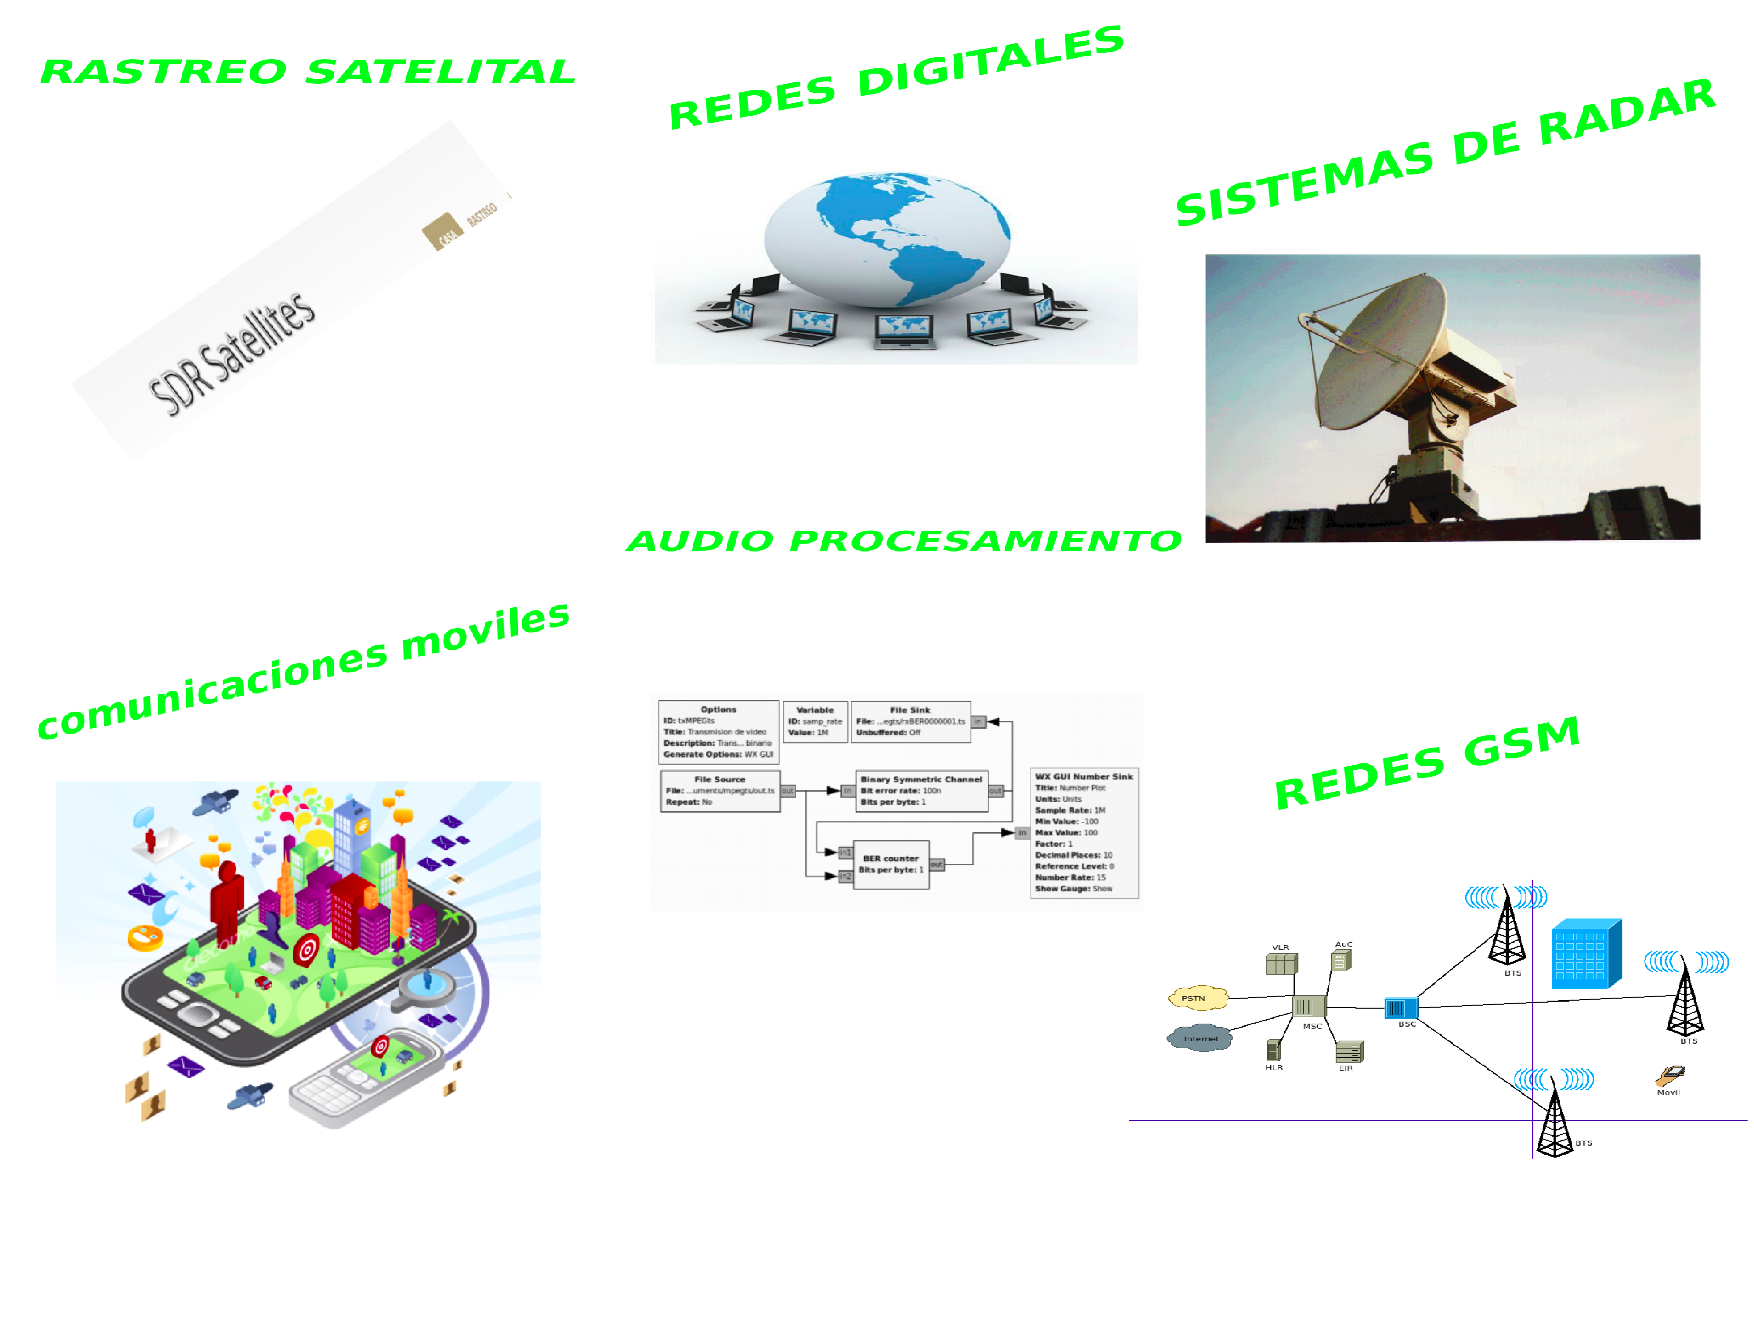
\includegraphics[width=0.9\textwidth]{parte1/intro/pdf/intro.pdf}
  \end{figure}
  
  
\end{frame}



\begin{frame}{Instalación de GNU Radio en Linux}
{Para instalar GNU Radio se deben seguir los siguientes pasos:}
\begin{enumerate}[1.]
\item Ingresar a la ventana de órdenes (o terminal) del sistema de su equipo.
\item Estando conectado a internet, escriba dentro del terminal:

  \begin{block}{}
  \texttt{
    sudo apt-get install gnuradio}
  \end{block}

\item Si su dispositivo tiene contrase\~na, debe ingresarla, al ser solicitada y oprimir \keys{\return}. 
\item Luego se deben aceptar los términos de la instalación oprimiendo la letra \keys{s} seguido de \keys{\return}. 
\item Una forma de verificar la correcta instalación es volviendo a ingresar el comando indicado en el punto 2, y si aparece un mensaje anunciando que GNU Radio ya está en su versión más reciente, su instalación fue correcta.
\end{enumerate}
\end{frame}
%----------------------------

\begin{frame}{Paquetes\index{Paquetes}}
Con el objetivo de clonar el repositorio y obtener los ejemplos de GNU Radio en nuestro ordenador se deben instalar los siguientes paquetes: 
  \begin{itemize}
  \item {BUILD-ESSENTIAL\\}
    \begin{itemize}
    \item
    {Build essential es un paquete que contiene herramientas necesarias
    para la creación, compilación e instalación de programas.}
    \end{itemize}
  \item {CMAKE\\}
  {Es un sistema de construcción de código abierto multiplataforma. Se trata de  un conjunto de herramientas diseñadas para construir, testear y empaquetar software. Se utiliza para controlar el proceso de compilación de software utilizando una plataforma sencilla y unos archivos de configuración
independientes del compilador.}
  \end{itemize}
\end{frame}
%-------------------------------

\begin{frame}{Paquetes}
  \begin{itemize}
  \item {GIT\\}
  \begin{itemize}
    \item
    {Este paquete contiene una Git; es un sistema de control de versiones distribuidas de código abierto desarrollado originalmente por Linux Torvalds para apoyar el desarrollo del kernel de Linux.}
    \item
    {El control de versiones es un sistema que registra los cambios realizados sobre un archivo o conjunto de archivos a lo largo del tiempo, de modo que se puedan recuperar versiones específicas más adelante.}
    \end{itemize}
  \item {LIBBOOST-ALL-DEV\\}
  {Es una biblioteca de software libre y revisión por partes preparadas para extender las capacidades del lenguaje de programación; permite ser utilizada en cualquier tipo de proyectos.}
  \end{itemize}
\end{frame}

%++++++++++++++++++++

\begin{frame}{Paquetes\index{Paquetes}}
  \begin{itemize}
  \item {LIBCPPUNIT-DEV\\}
  \begin{itemize}
    \item
    {Biblioteca de pruebas unitarias para C++.}
    \item
    {Una prueba unitaria es una forma de comprobar el correcto
funcionamiento de una unidad de código. Por ejemplo, en diseño
estructurado o en diseño funcional, una función o un procedimiento,
en diseño orientado a objetos una clase. Esto sirve para asegurar que
cada unidad funcione correcta y eficientemente por separado.}
    \end{itemize}
  \item {DOXYGEN\\}
  {Es una herramienta para generar documentación a partir de código fuente. Es un sistema de documentación para C++, C, Java, Python. Es necesario solo si se desea generar referencias a documentación externa de la que no tiene las fuentes.}
  \end{itemize}
\end{frame}

%+++++++++++++++++++

\begin{frame}{Instalación de paquetes}
\begin{enumerate}[1.]
\item La instalación de cada uno se los paquetes anteriormente mencionados, se realiza colocando, en la ventana de terminal, las siguientes órdenes:
\end{enumerate}

  \begin{block}{}
  \texttt{
  \ \ \ sudo apt-get install build-essential
    \begin{itemize}
      \item[] sudo apt-get install cmake
      \item[] sudo apt-get install git
      \item[] sudo apt-get install libboost-all-dev
      \item[] sudo apt-get install libcppunit-dev
      \item[] sudo apt-get install doxygen
    \end{itemize}}
  \end{block}


\end{frame}

%++++++++++++++++++++


\begin{frame}{Clonar repositorio\index{Clonar Repositorio}}
El código fuente de los ejemplos está almacenado en github por lo tanto para clonar el repositorio se debe realizar lo siguiente:
\begin{itemize}
\item Abrir la ventana de órdenes o terminal.
\item Después se debe ingresar el siguiente comando para clonar el directorio git:

\begin{block}{}
  \texttt{
    git clone https://github.com/gnuradio/gr-tutorial}
  \end{block}

\item Una vez clonado el directorio se deben ver exactamente los mismos archivos y carpetas que los del repositorio github, en el PC empleado.
\end{itemize}
\end{frame}

%+++++++++++++++++++

\begin{frame}{Instalación de módulos\index{Modulos}}
\begin{itemize}
\item Luego de haber clonado el repositorio, debemos buscar la carpeta de gr-tutorial e ingresar a ella desde el terminal, para ello se digitan los siguientes mandos:

  \begin{block}{}
  \texttt{
  \ \ \ ls
    \begin{itemize}
      \item[] cd gr-tutorial
    \end{itemize}}
  \end{block}

Es importante mencionar que al escribir el primer comando se podrán observar la diferentes carpetas que se encuentran en el dispositivo, por lo tanto gr-tutorial debe aparecer entre las opciones para poder cambiar de directorio. 
\end{itemize}
\end{frame}

%+++++++++++++++

\begin{frame}{Instalación de módulos\index{Modulos}}
\begin{itemize}
\item Estando dentro de la carpeta, desde la terminal, se deben escribir los siguientes comandos, con la finalidad de instalar las soluciones o módulos:

  \begin{block}{}
  \texttt{
  \ \ \ mkdir build
    \begin{itemize}
      \item[] cd build
      \item[] cmake ..
      \item[] make -j8
      \item[] sudo make install
      \item[]sudo ldconfig
    \end{itemize}}
  \end{block}

\end{itemize}
\end{frame}


%///////////////////////////////////////////////////////////////
\subsection{Grid position de WX GUI}
%*********************
\begin{frame}{}

\pgfdeclareimage[width=\paperwidth,height=\paperheight]{bg}{imagenes/fondo_lab}
\setbeamertemplate{background}{\pgfuseimage{bg}}

\bfseries{\textrm{\LARGE Grid position de \newline WX GUI}}
\raggedright
\end{frame}
%*********************

\begin{frame}{Grid position}

\pgfdeclareimage[width=\paperwidth,height=\paperheight]{bg}{imagenes/fondo3}
\setbeamertemplate{background}{\pgfuseimage{bg}}

\textbf {Posicionamiento de rejilla} \\
\vspace{2mm}
GRC ofrece varios receptores gráficos y controles gráficos para crear gráficos de flujo wx-gui.(scope sink, fft sink, number sink, waterfall sink, constellation sink, slider control, and chooser control) Cada uno de estos elementos gráficos tiene un parámetro de posición de cuadrícula para un posicionamiento preciso.

\end{frame}
%-----------------------------------

\begin{frame}{Grid position}

\begin{figure}[H]
\centering
\vspace{-3mm}
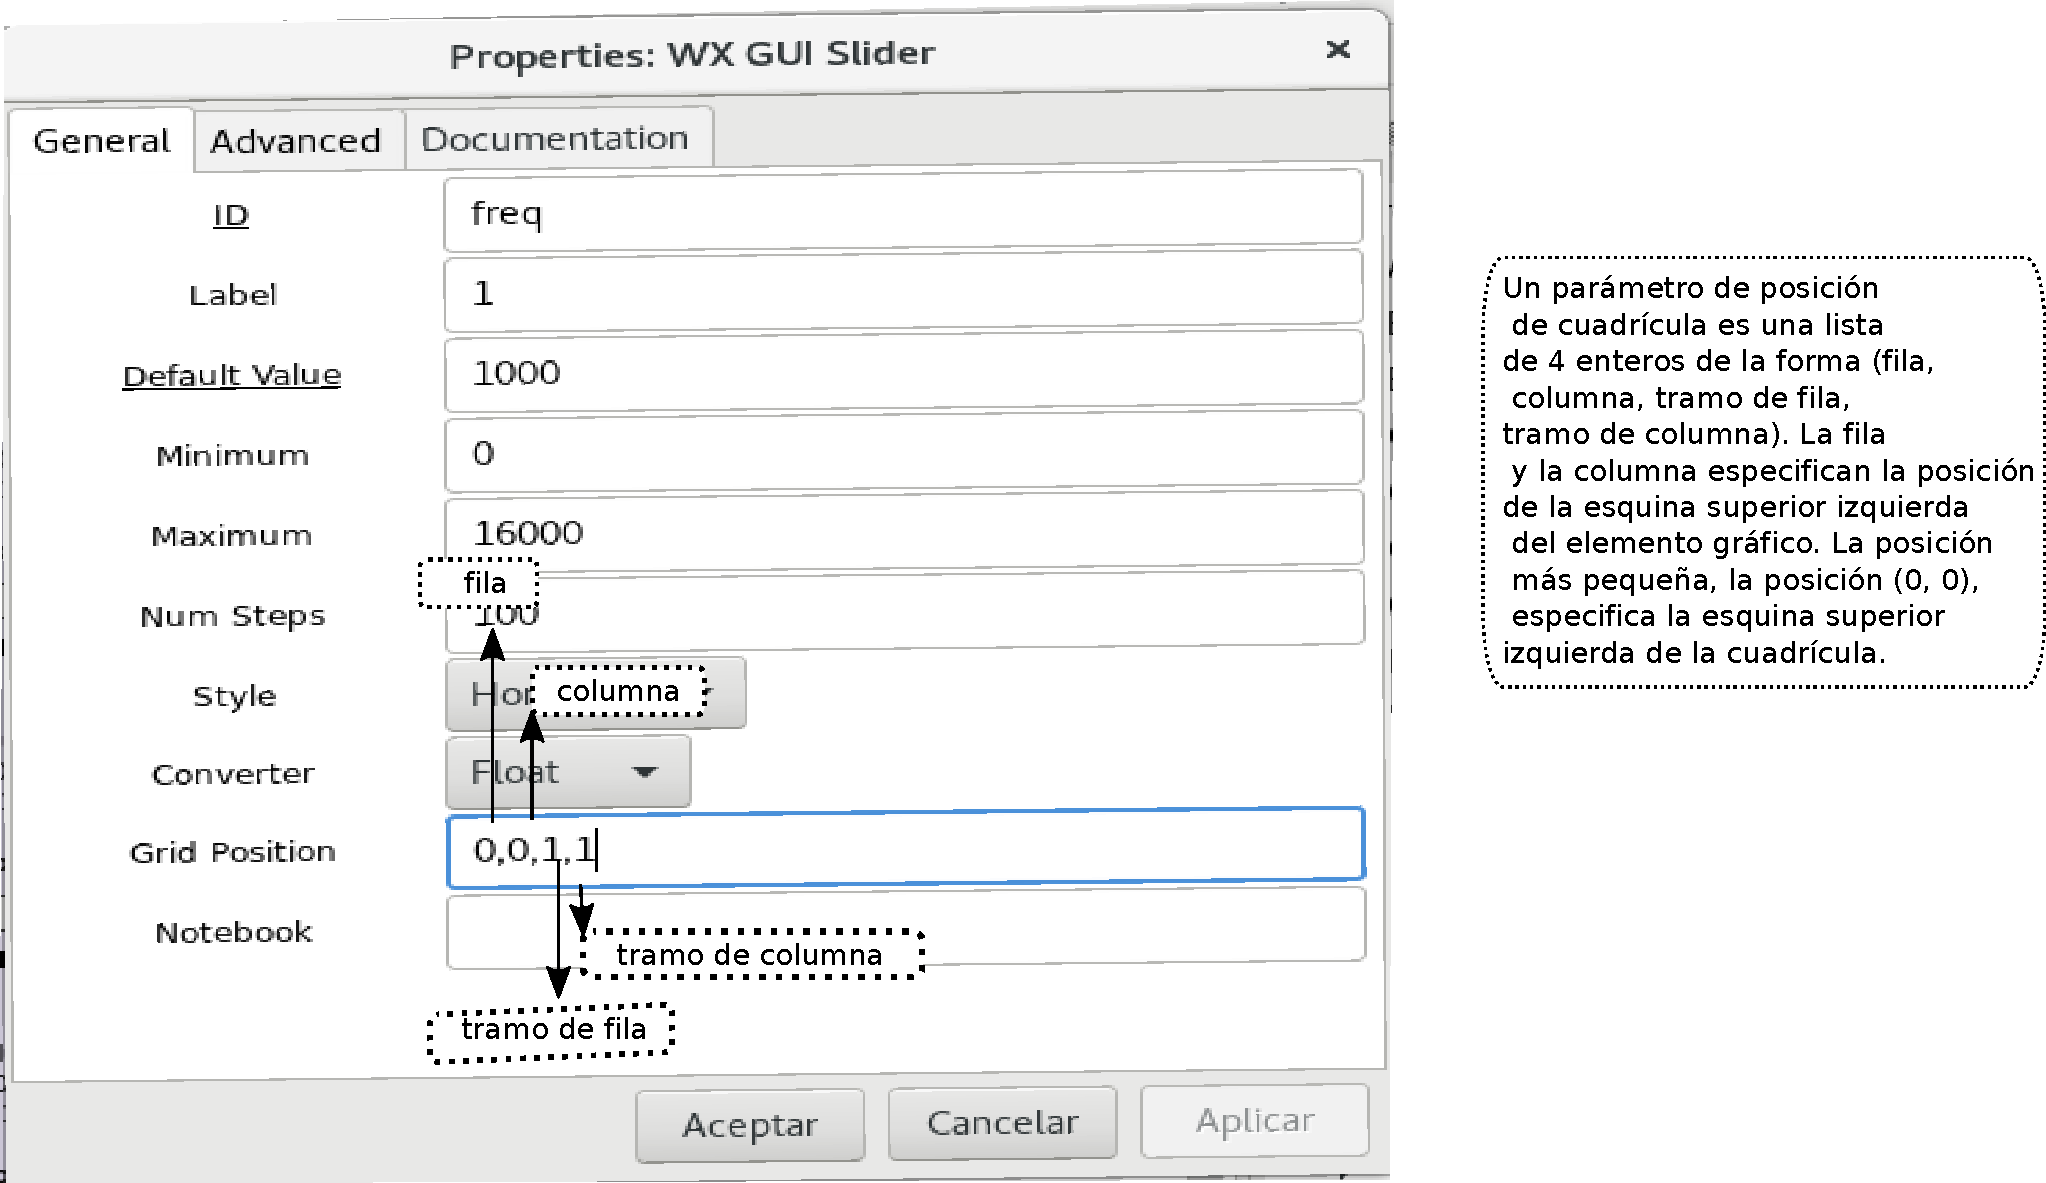
\includegraphics[width=0.9\textwidth]{parte1/lab00/pdf/lab0_1.pdf}


\end{figure}

\end{frame}
%-----------------------------------

\begin{frame}{Grid position}

El tramo de fila especifica el número de filas hacia abajo desde la posición de la fila, y el tramo de columna especifica el número de columnas a la derecha de la posición de la columna. Por lo tanto, el tramo debe ser al menos (1, 1) para ocupar el mínimo de 1 celda de cuadrícula.

\end{frame}
%-----------------------------------

\begin{frame}{Grid position}

\begin{figure}[H]
\centering
\vspace{-3mm}
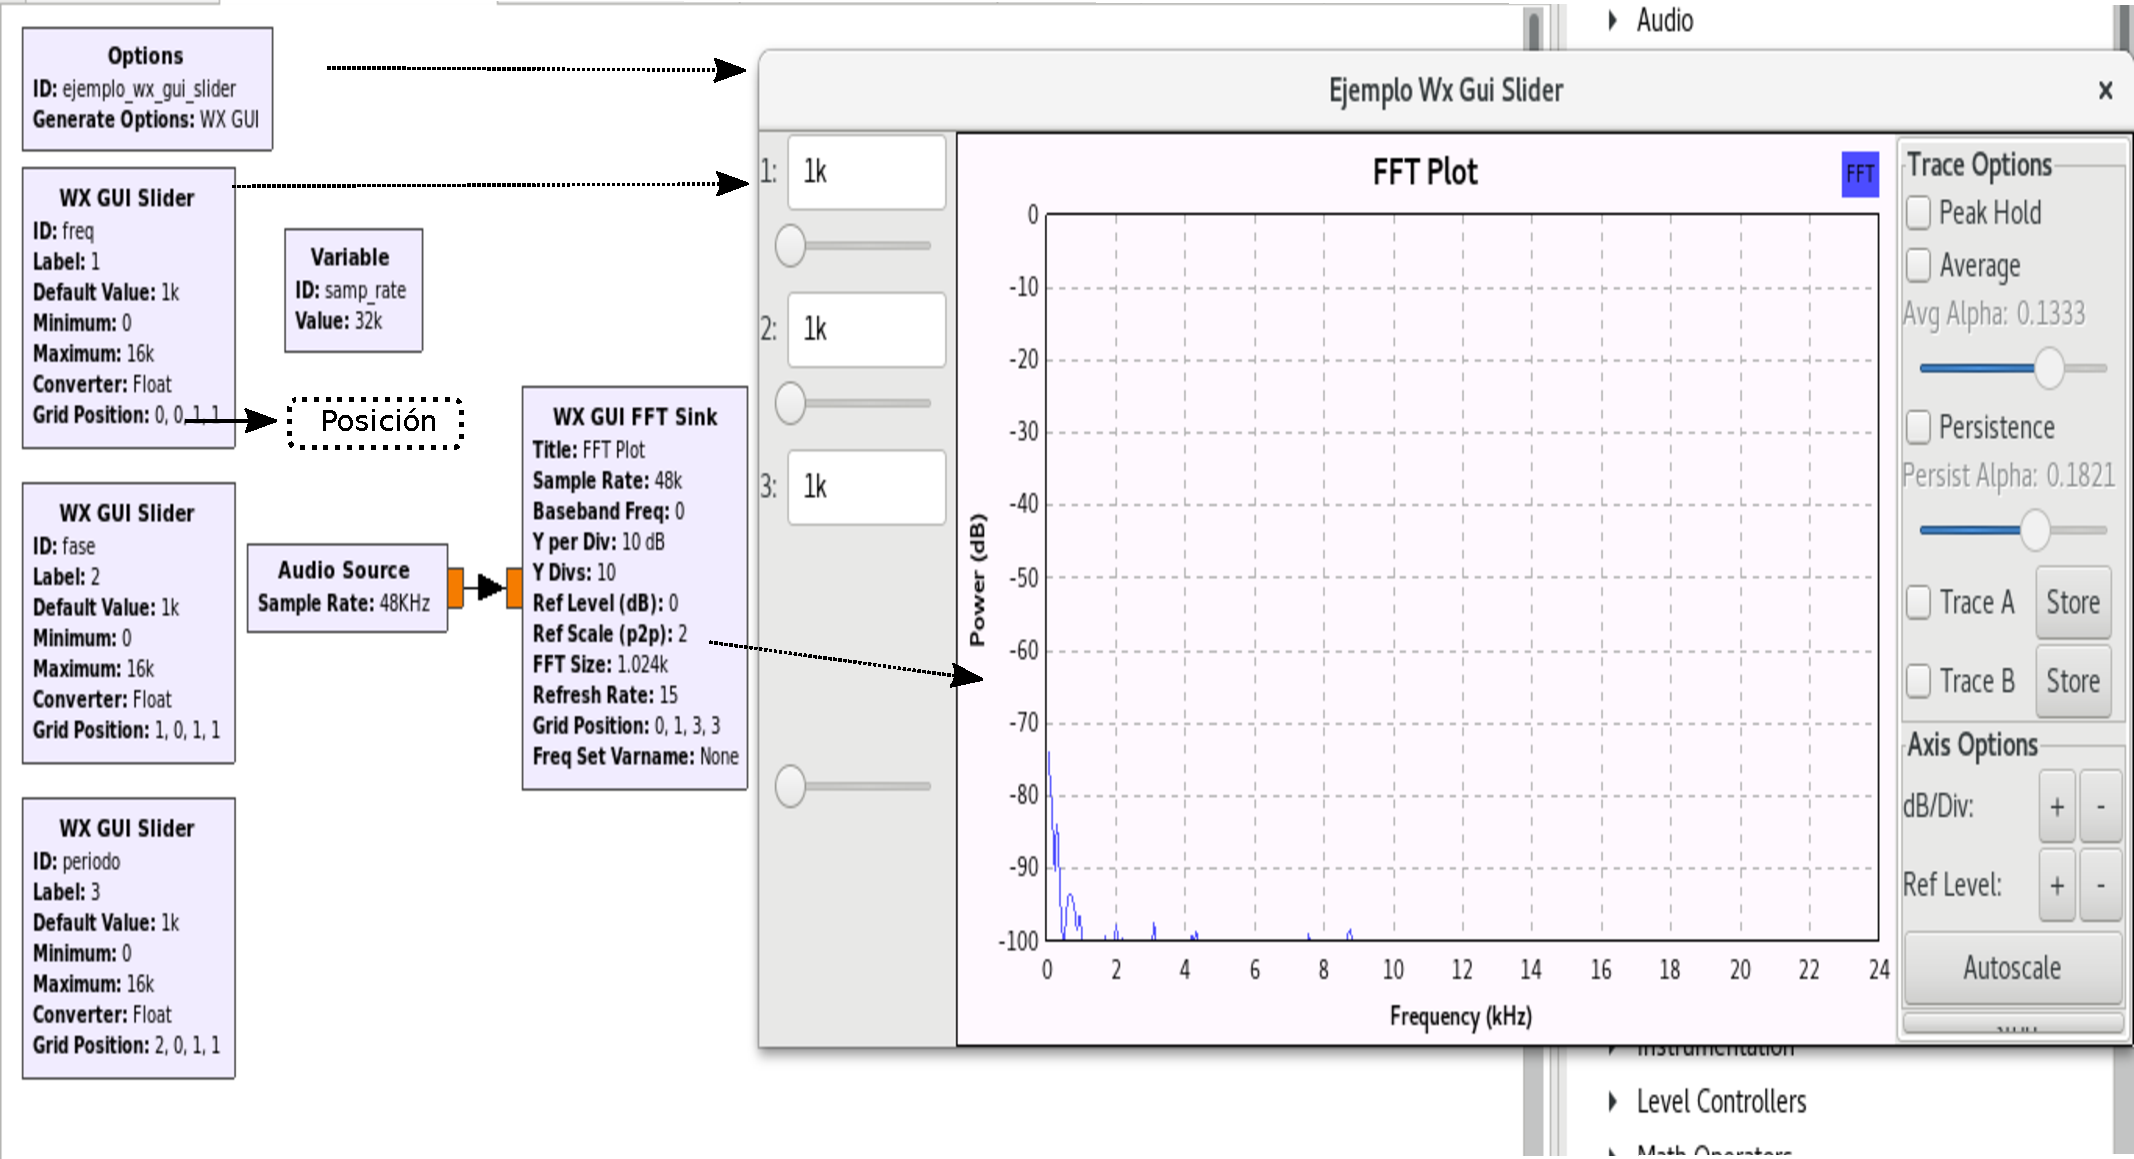
\includegraphics[width=0.9\textwidth]{parte1/lab00/pdf/lab0_2.pdf}
\end{figure}

\end{frame}
%-----------------------------------

\begin{frame}{Grid position}

\begin{figure}[H]
\centering
\vspace{-3mm}
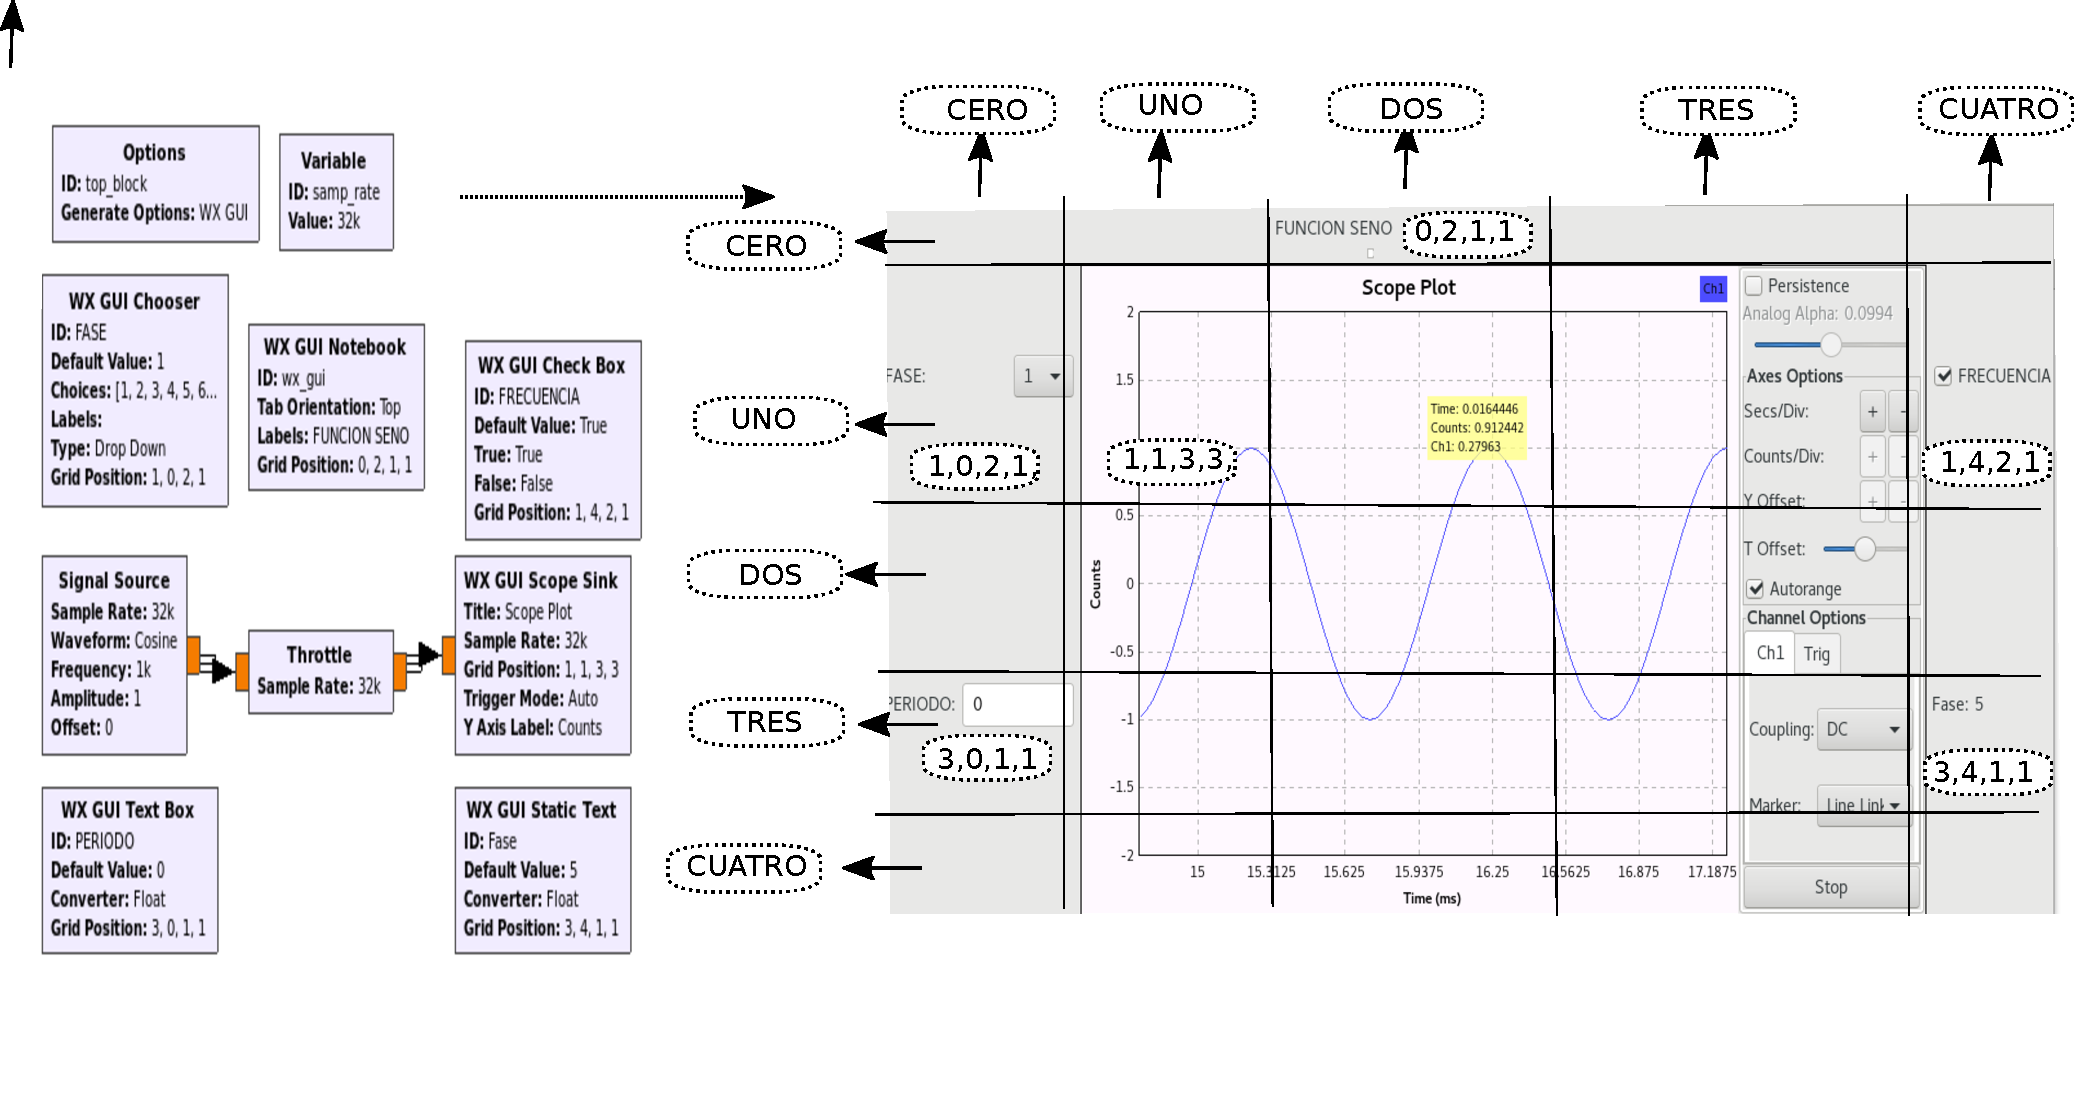
\includegraphics[width=0.9\textwidth]{parte1/lab00/pdf/lab0_3.pdf}
\end{figure}

\end{frame}
%-----------------------------------


%///////////////////////////////////////////////////////////////
\subsection{Lab1: Primeros pasos}
%*********************
\begin{frame}{}

\pgfdeclareimage[width=\paperwidth,height=\paperheight]{bg}{imagenes/fondo_lab}
\setbeamertemplate{background}{\pgfuseimage{bg}}

\bfseries{\textrm{\LARGE Lab1\\ \Large Primeros pasos}}
\raggedright
\end{frame}
%*********************

\begin{frame}{Primeros pasos}

\pgfdeclareimage[width=\paperwidth,height=\paperheight]{bg}{imagenes/fondo3}
\setbeamertemplate{background}{\pgfuseimage{bg}}

\begin{figure}[H]
\centering
\vspace{-3mm}
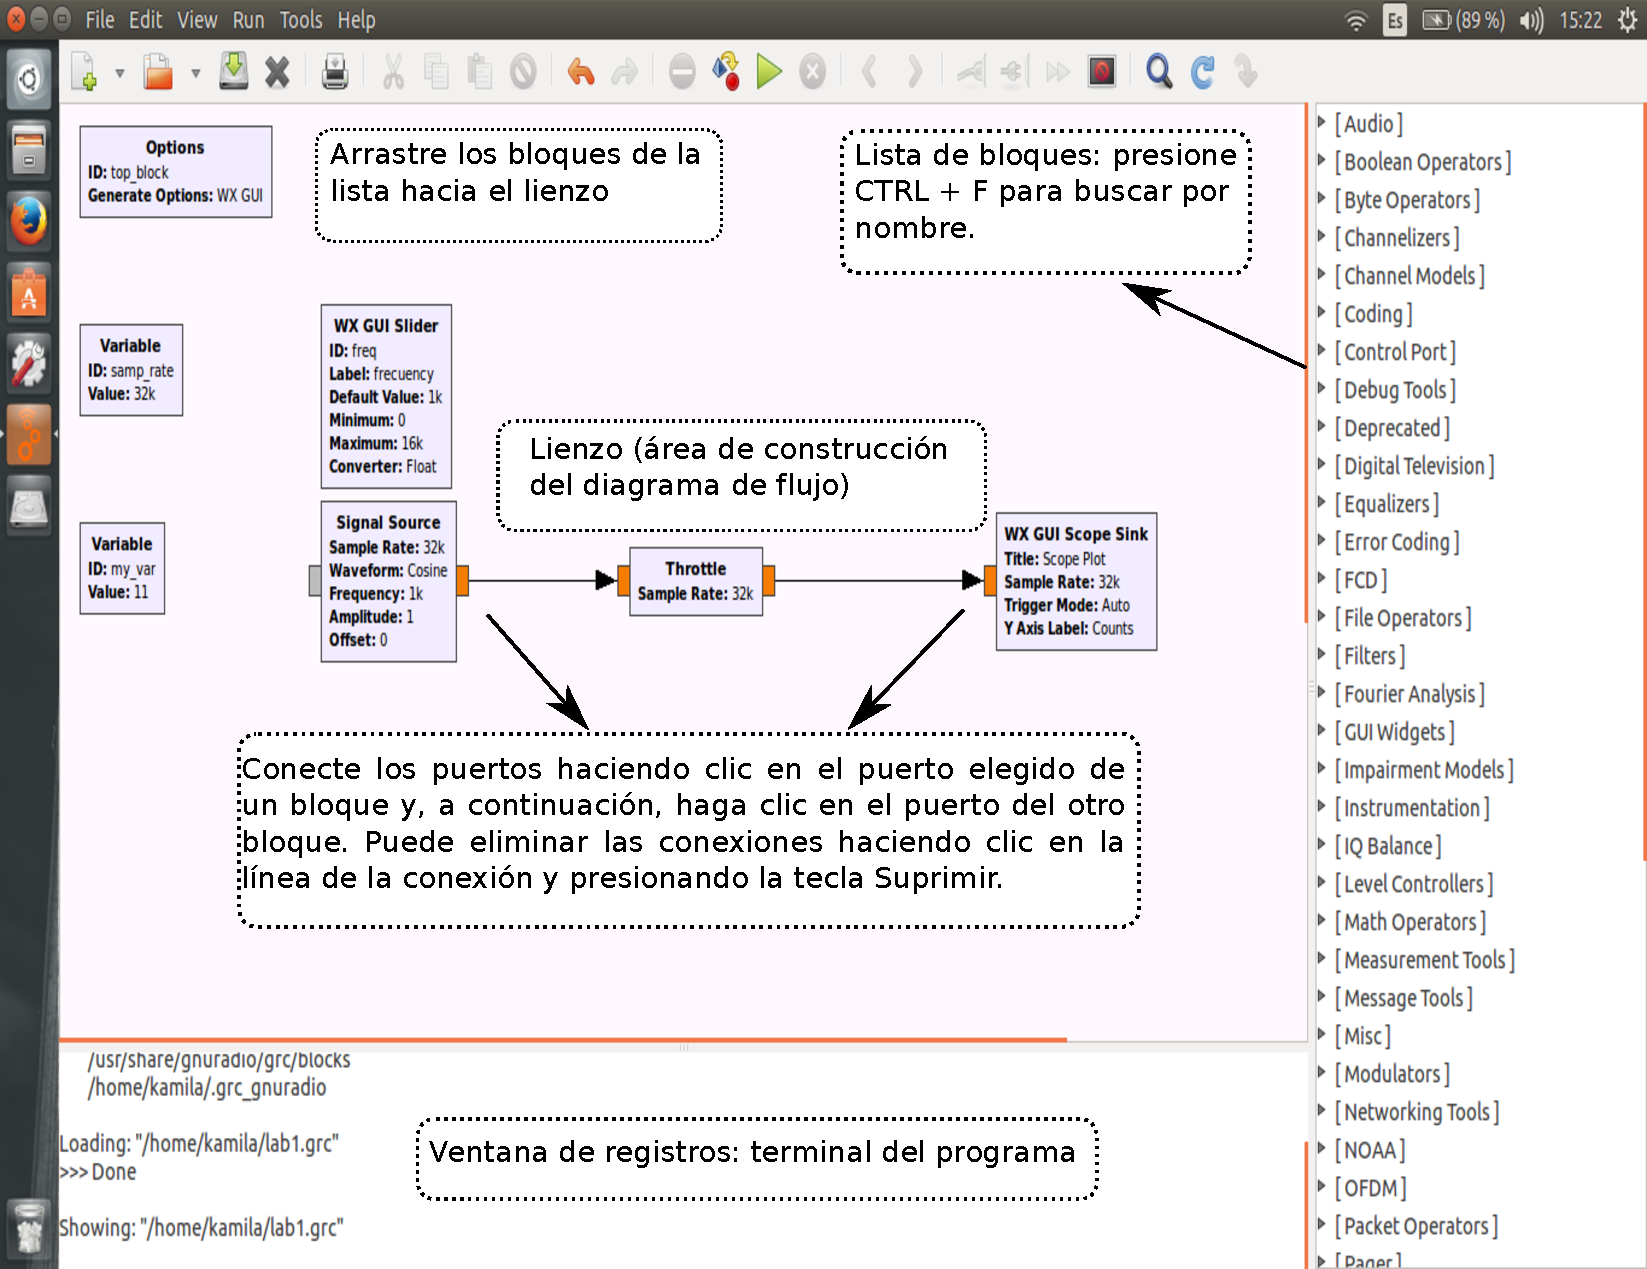
\includegraphics[width=0.9\textwidth]{parte1/lab1/pdf/lab1_1.pdf}
\end{figure}
\end{frame}
%-----------------------------------

\begin{frame}{Primeros pasos }
\begin{figure}[H]
\centering
\vspace{-3mm}
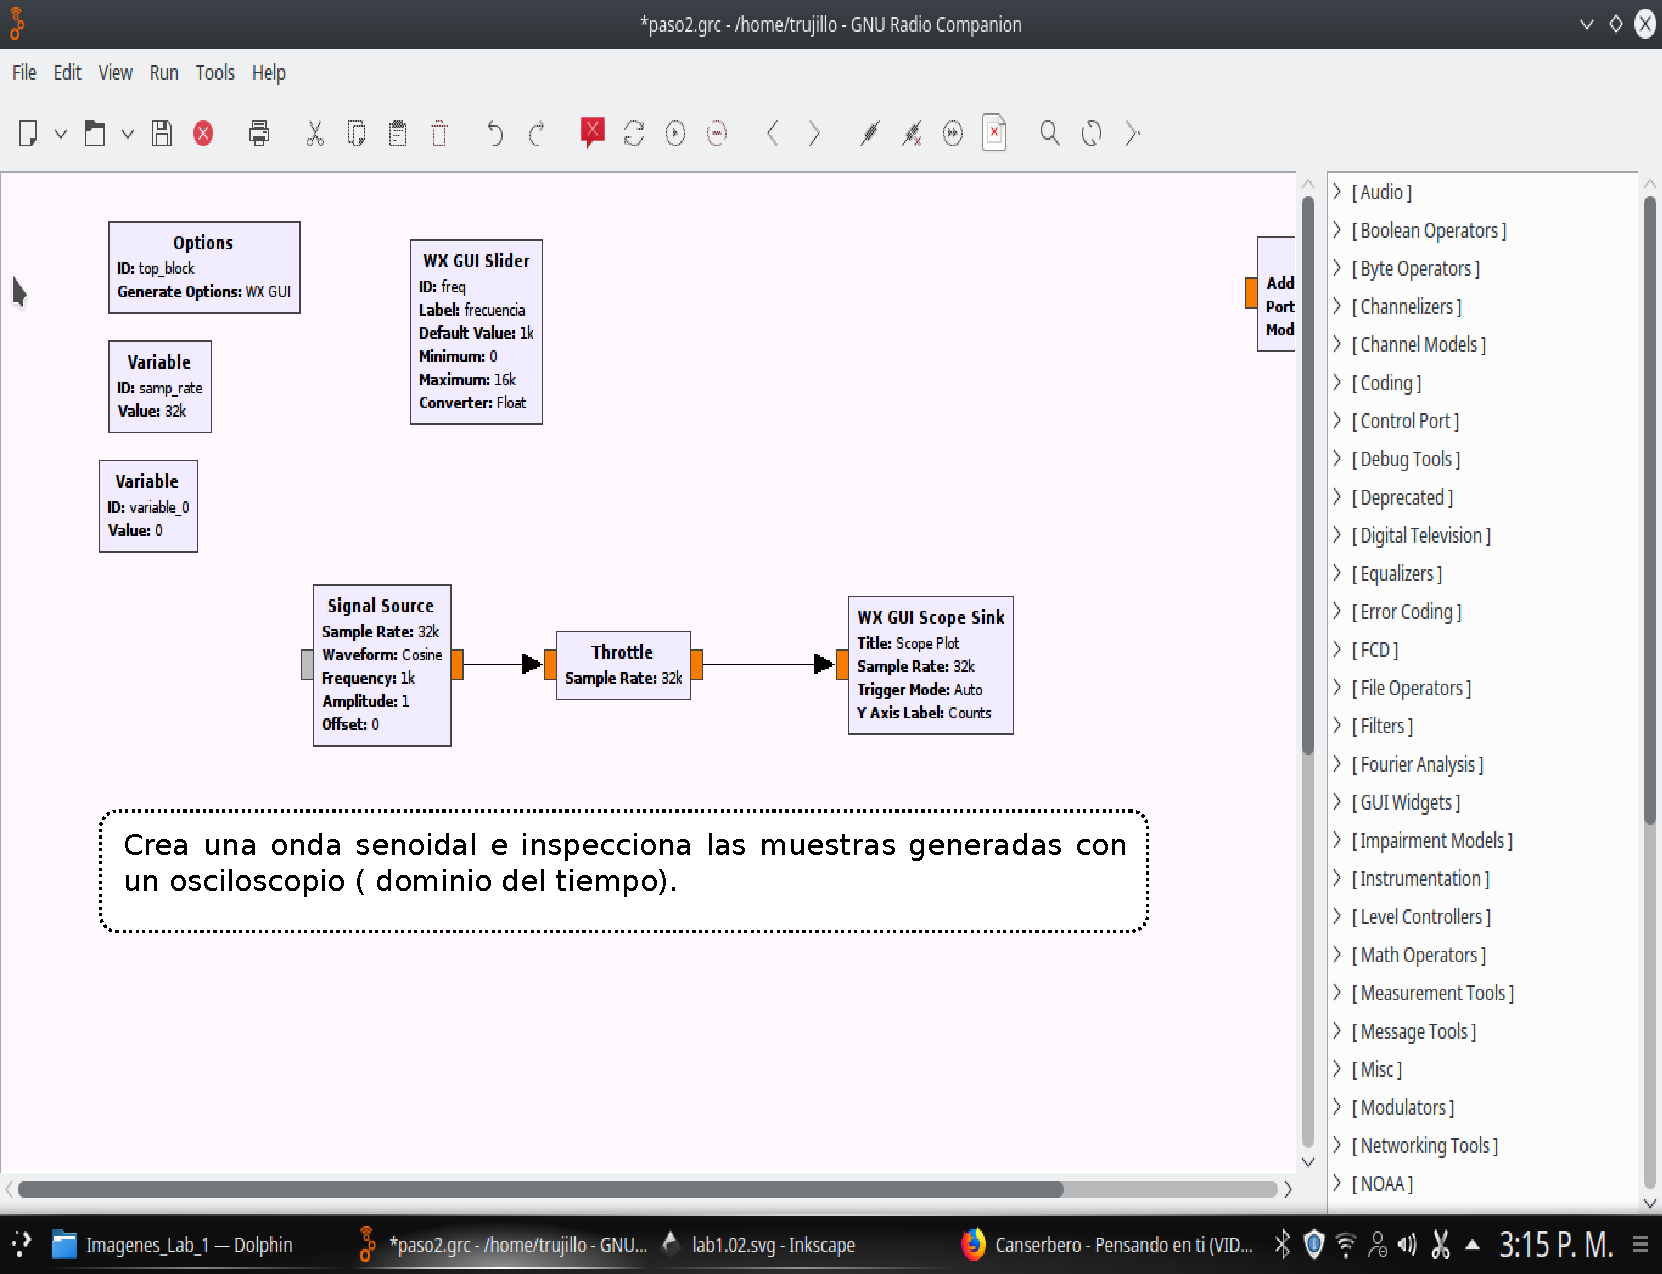
\includegraphics[width=0.9\textwidth]{parte1/lab1/pdf/lab1_2.pdf}
\end{figure}
\end{frame}
%-----------------------------------

\begin{frame}{Primeros pasos }
\begin{figure}[H]
\vspace{-3mm}
\centering
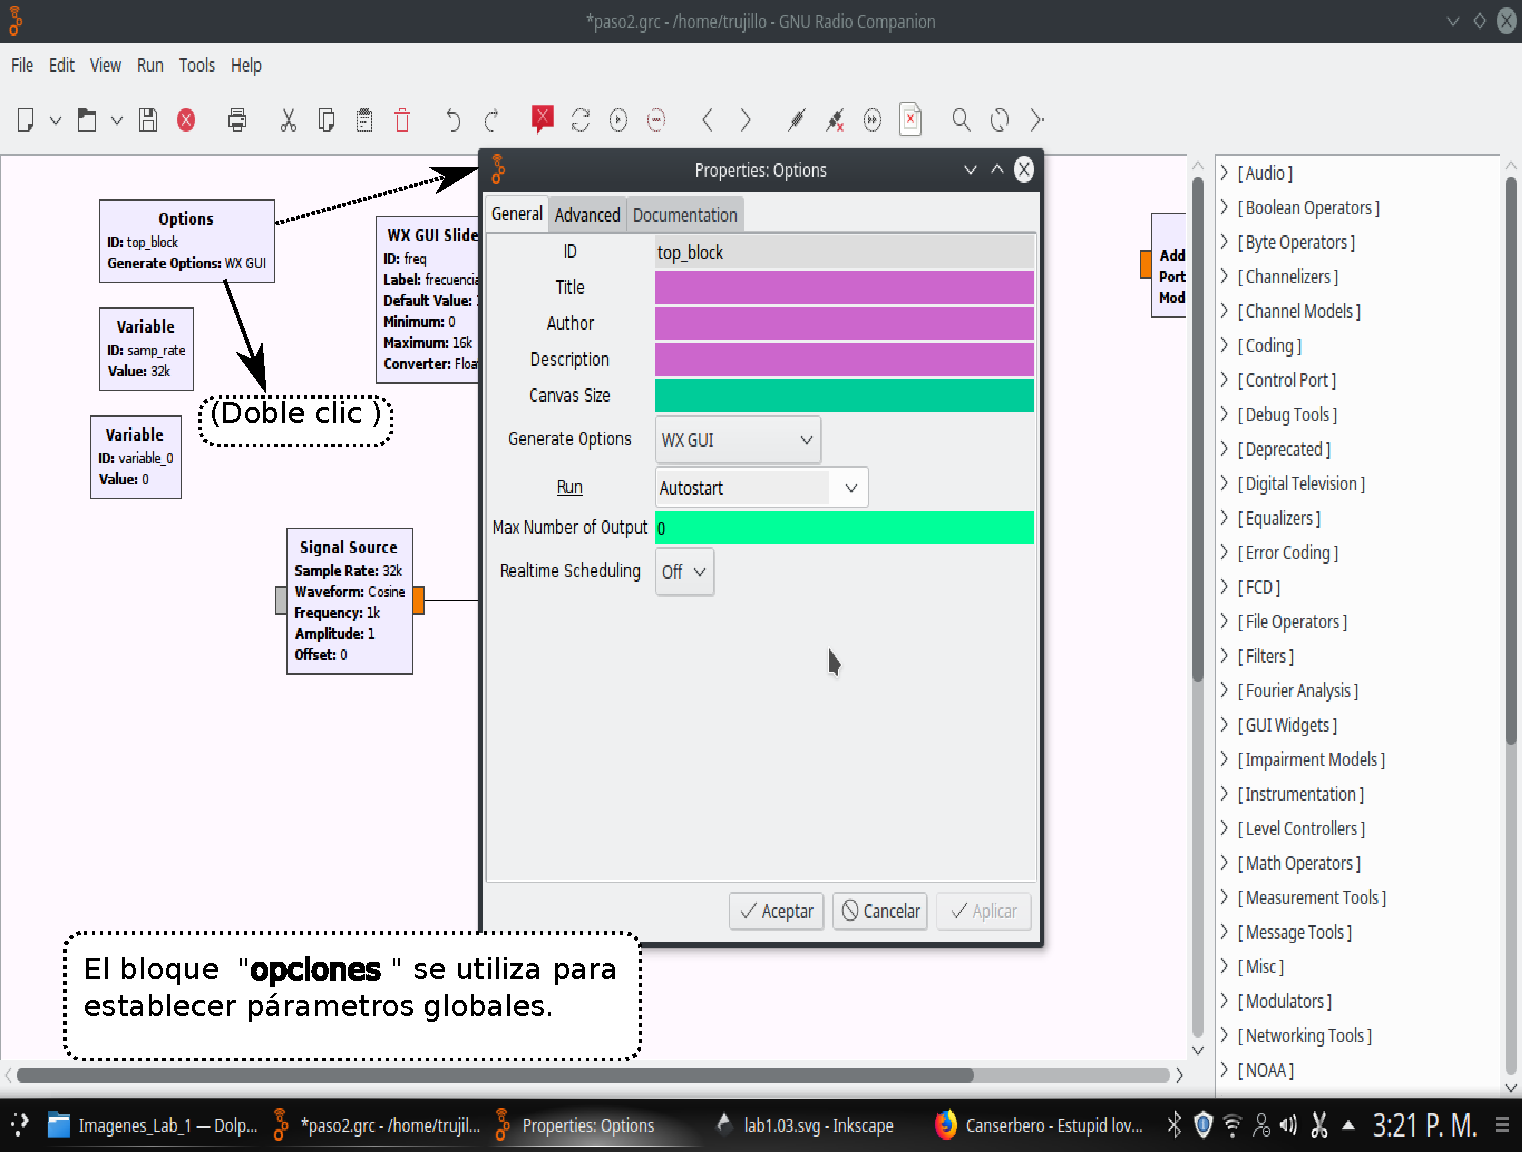
\includegraphics[width=0.9\textwidth]{parte1/lab1/pdf/lab1_3.pdf}
\end{figure}
\end{frame}
%-----------------------------------

\begin{frame}{Primeros pasos }
\begin{figure}[H]
\vspace{-3mm}
\centering
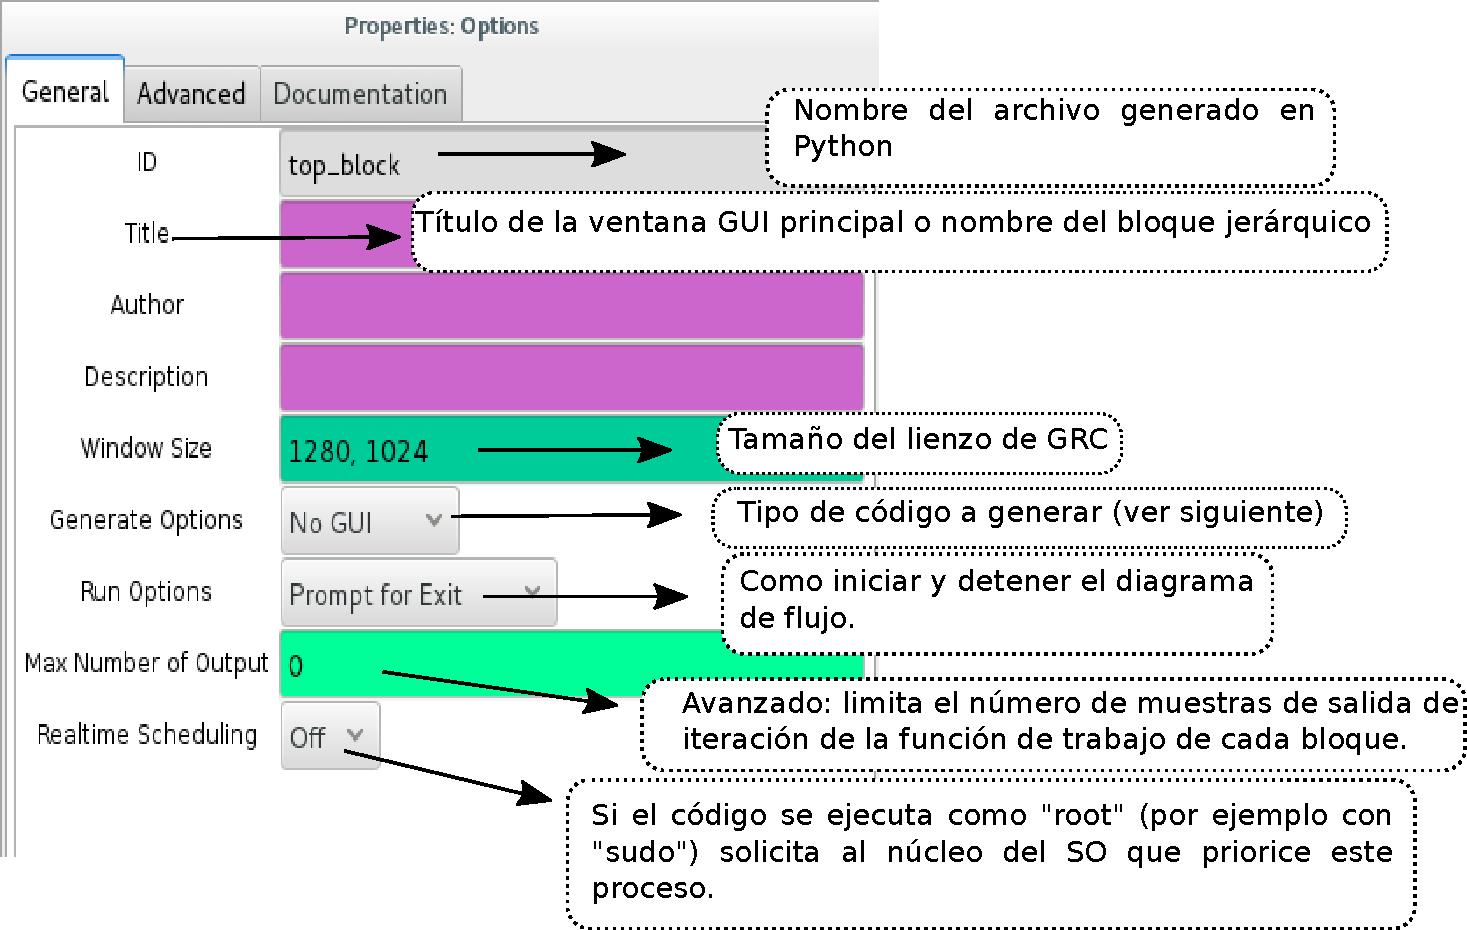
\includegraphics[width=0.9\textwidth]{parte1/lab1/pdf/lab1_4.pdf}
\end{figure}
\end{frame}
%-----------------------------------

\begin{frame}{Primeros pasos }
\begin{figure}[H]
\vspace{-2cm}
\centering
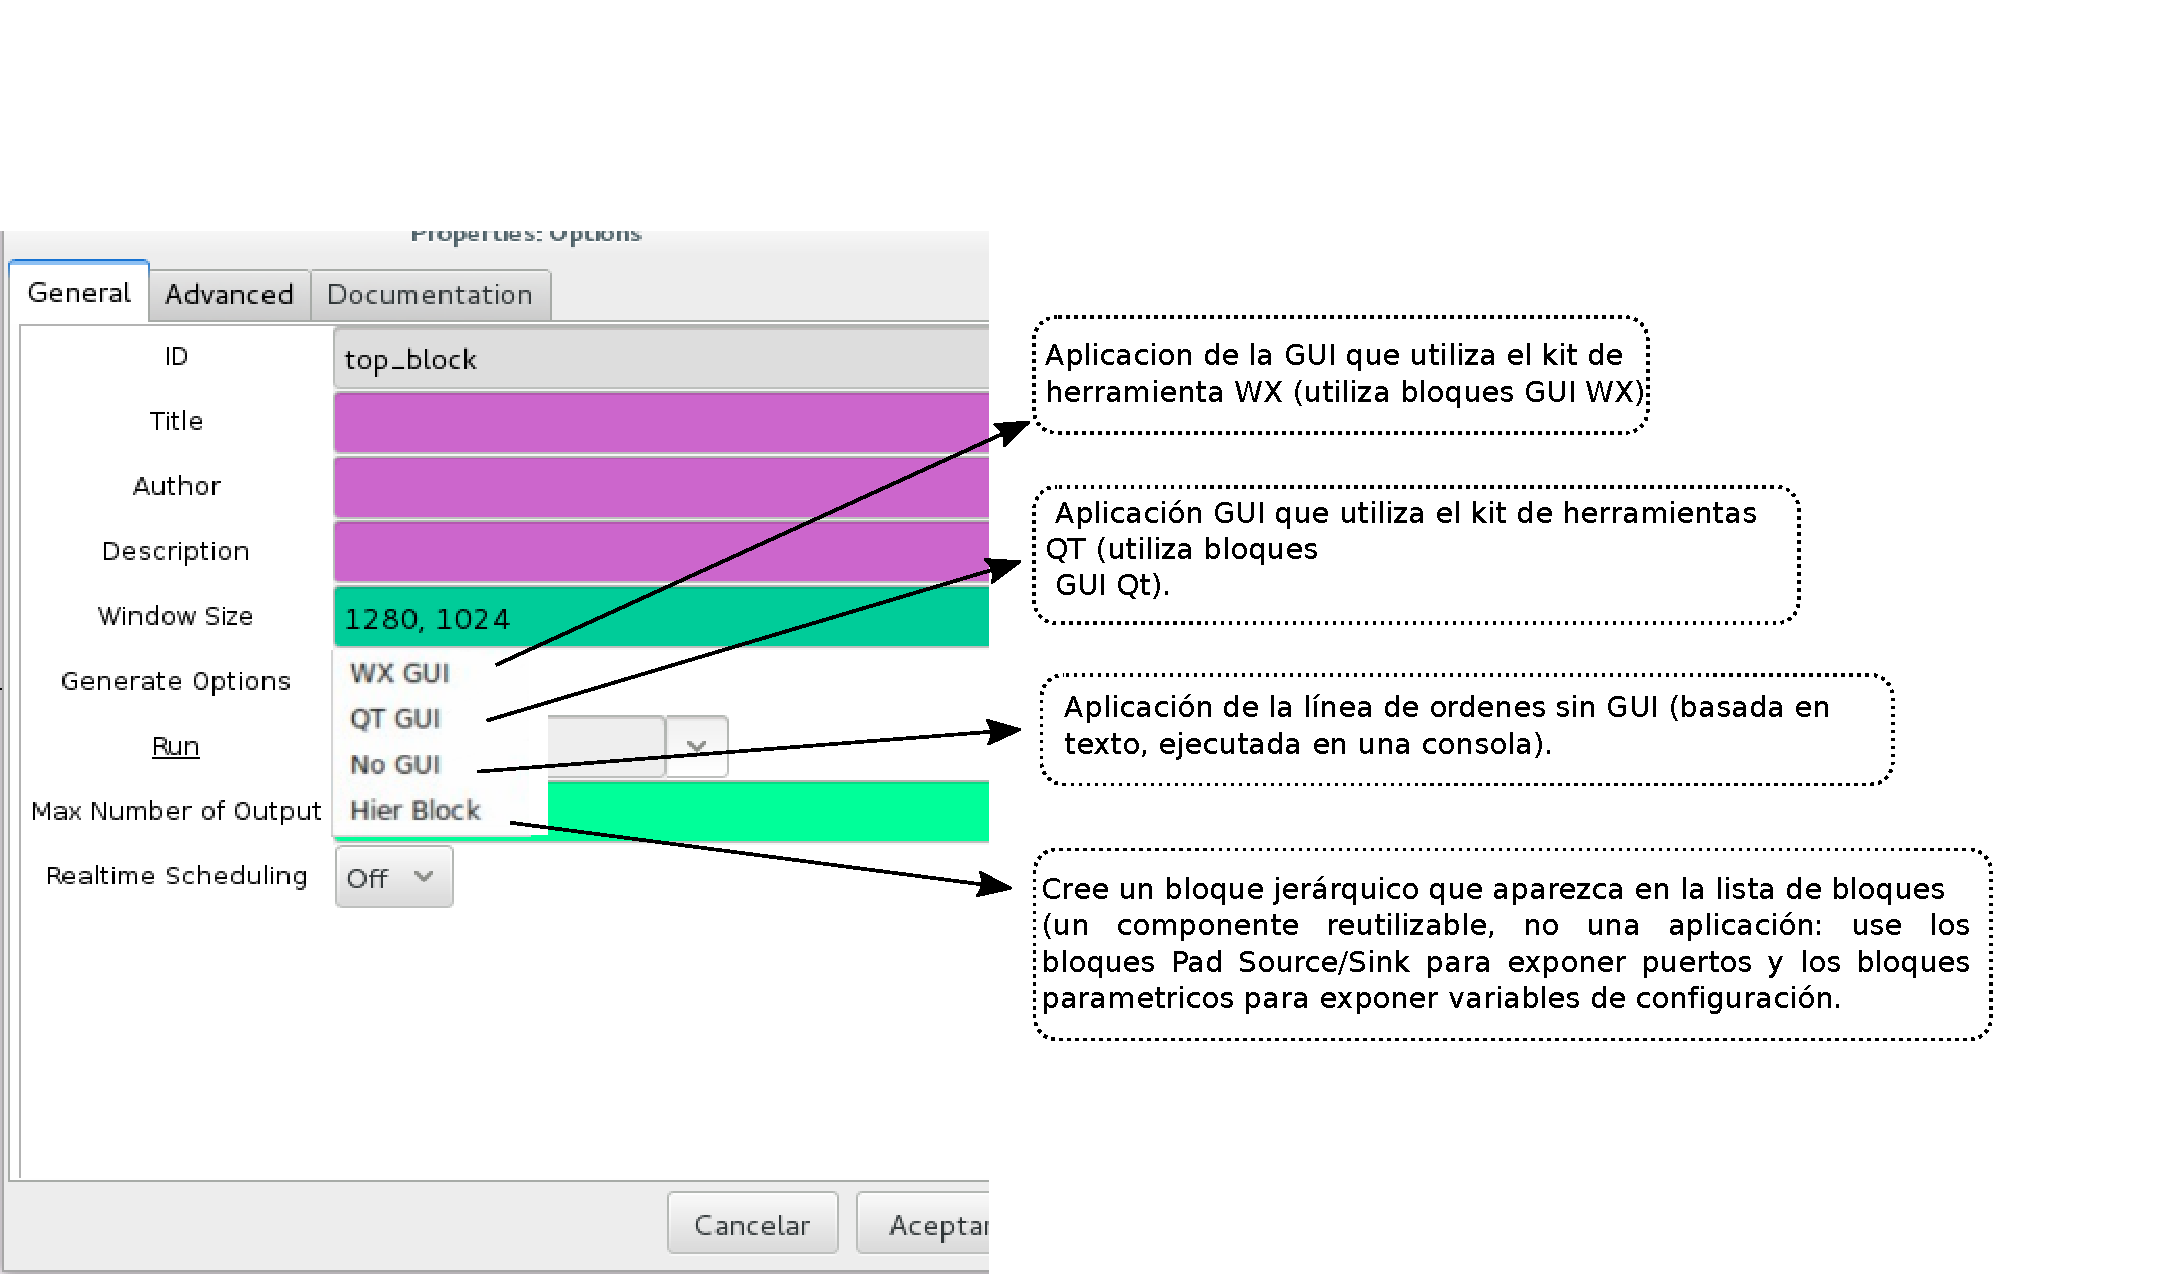
\includegraphics[width=1.1\textwidth]{parte1/lab1/pdf/lab1_5.pdf}
\end{figure}
\end{frame}
%-----------------------------------

\begin{frame}{Primeros pasos }
\begin{figure}[H]
\centering
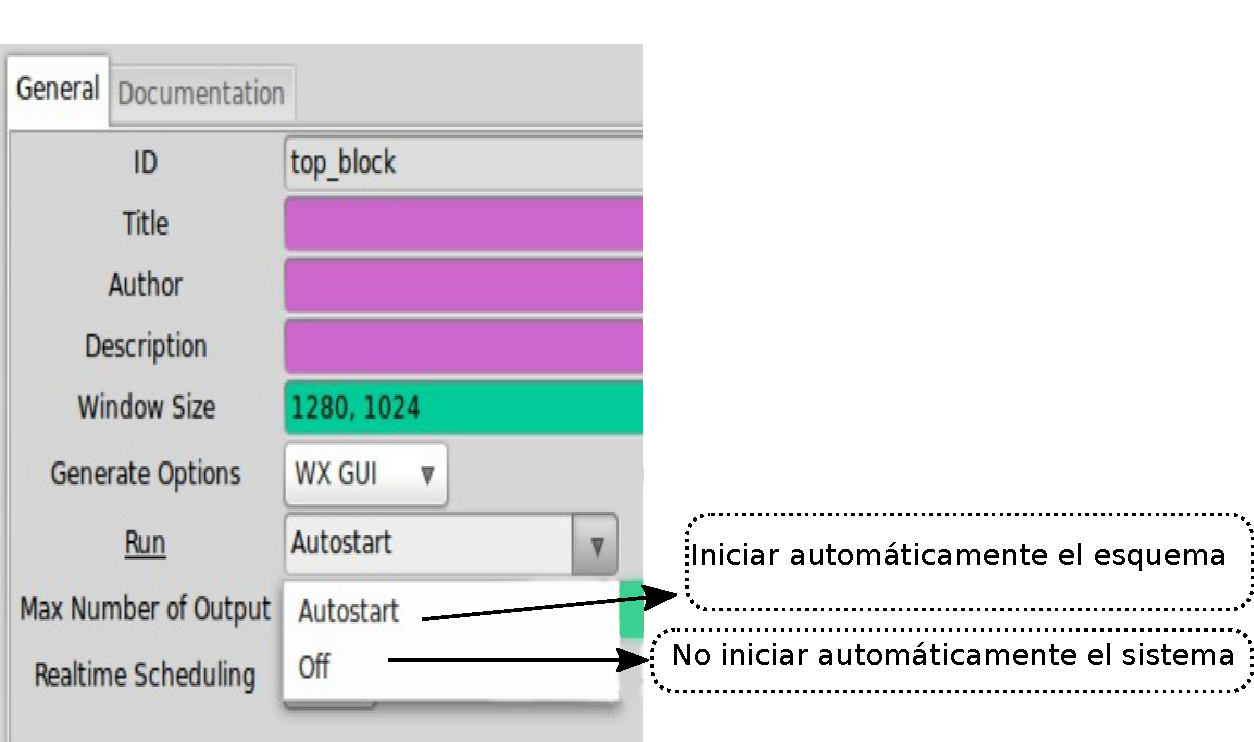
\includegraphics[width=.9\textwidth]{parte1/lab1/pdf/lab1_6.pdf}
\end{figure}
\end{frame}
%-----------------------------------

\begin{frame}{Primeros pasos }
\begin{figure}[H]
\centering
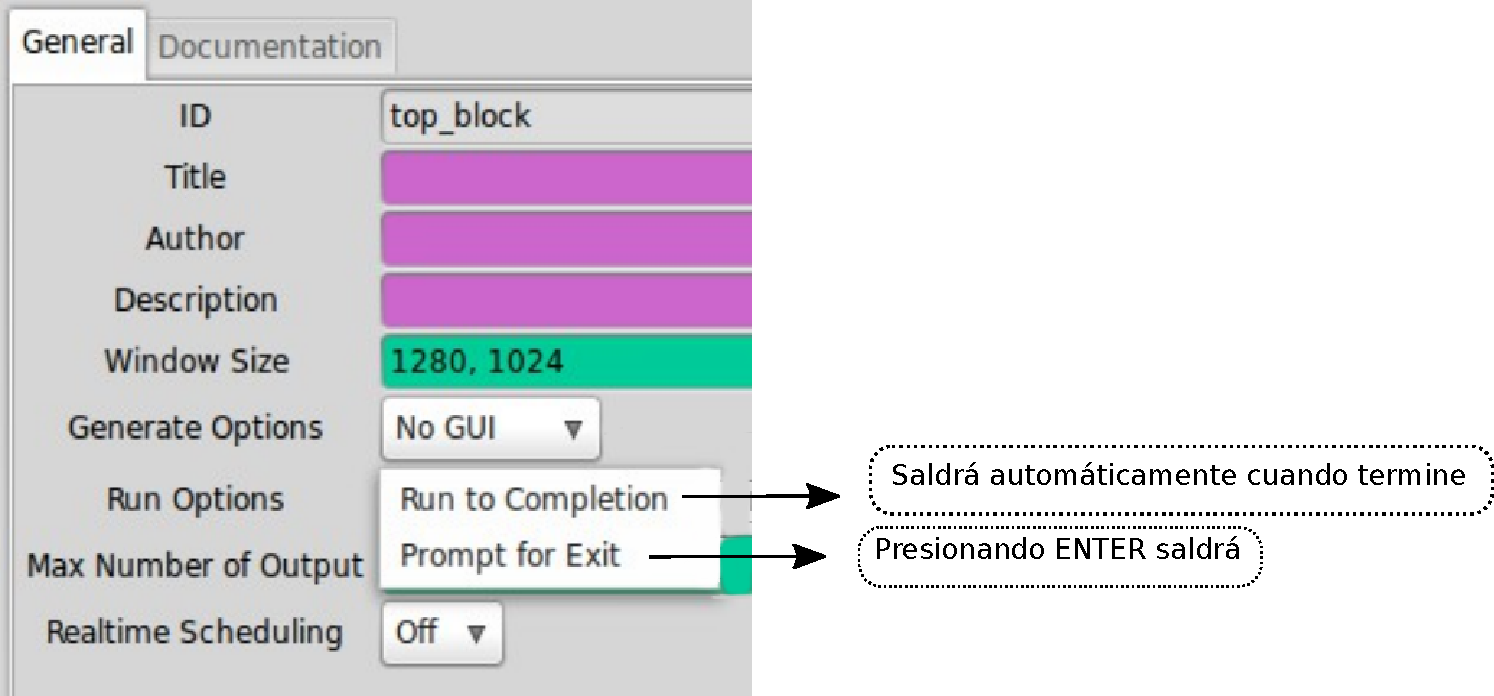
\includegraphics[width=\textwidth]{parte1/lab1/pdf/lab1_7.pdf}
\end{figure}
\end{frame}
%-----------------------------------

\begin{frame}{Primeros pasos }
\begin{figure}[H]
\vspace{-1cm}
\centering
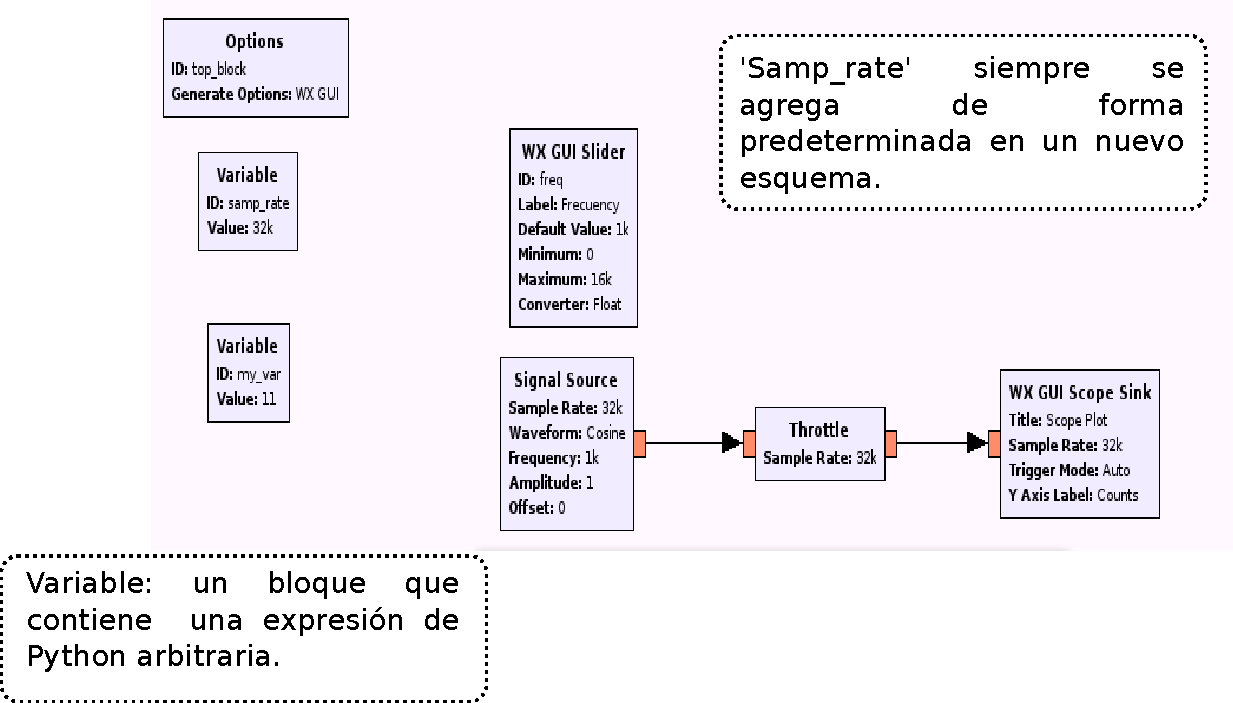
\includegraphics[width=\textwidth]{parte1/lab1/pdf/lab1_8.pdf}
\end{figure}
\end{frame}
%-----------------------------------

\begin{frame}{Primeros pasos }
\begin{figure}[H]
\vspace{-3mm}
\centering
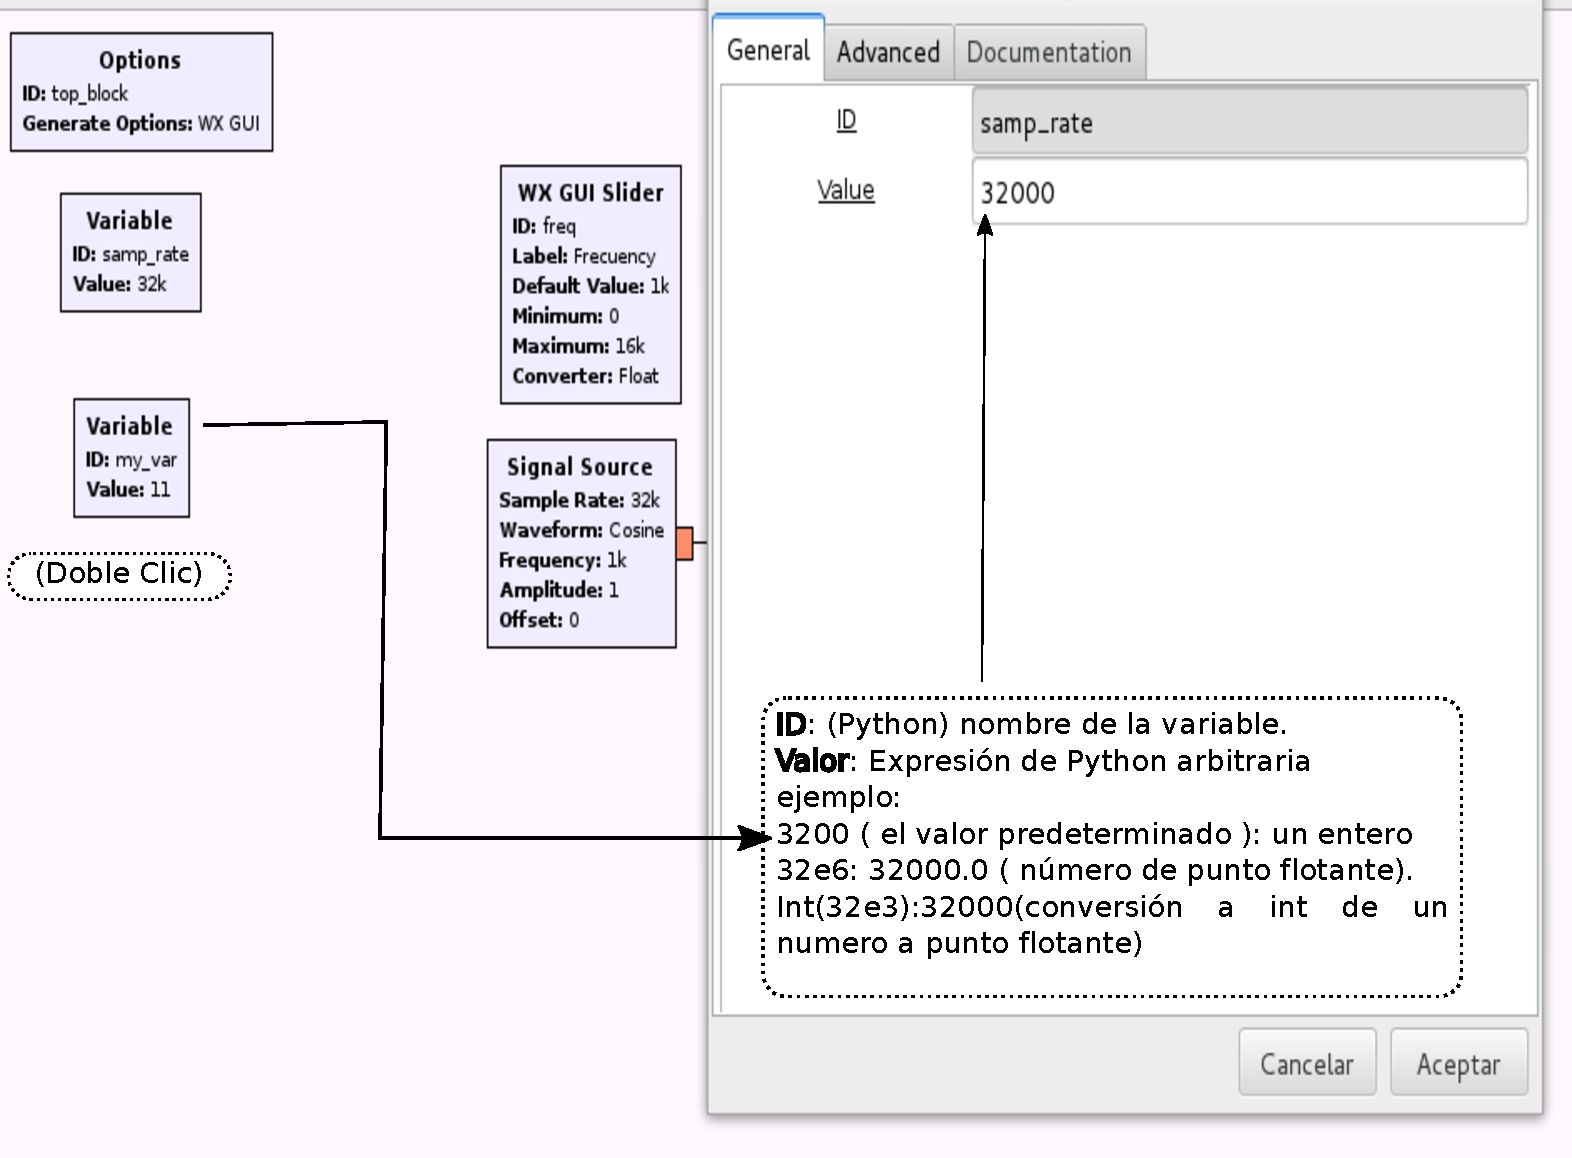
\includegraphics[width=0.85\textwidth]{parte1/lab1/pdf/lab1_9.pdf}
\end{figure}
\end{frame}
%-----------------------------------

\begin{frame}{Primeros pasos }
\begin{figure}[H]
\vspace{-3mm}
\centering
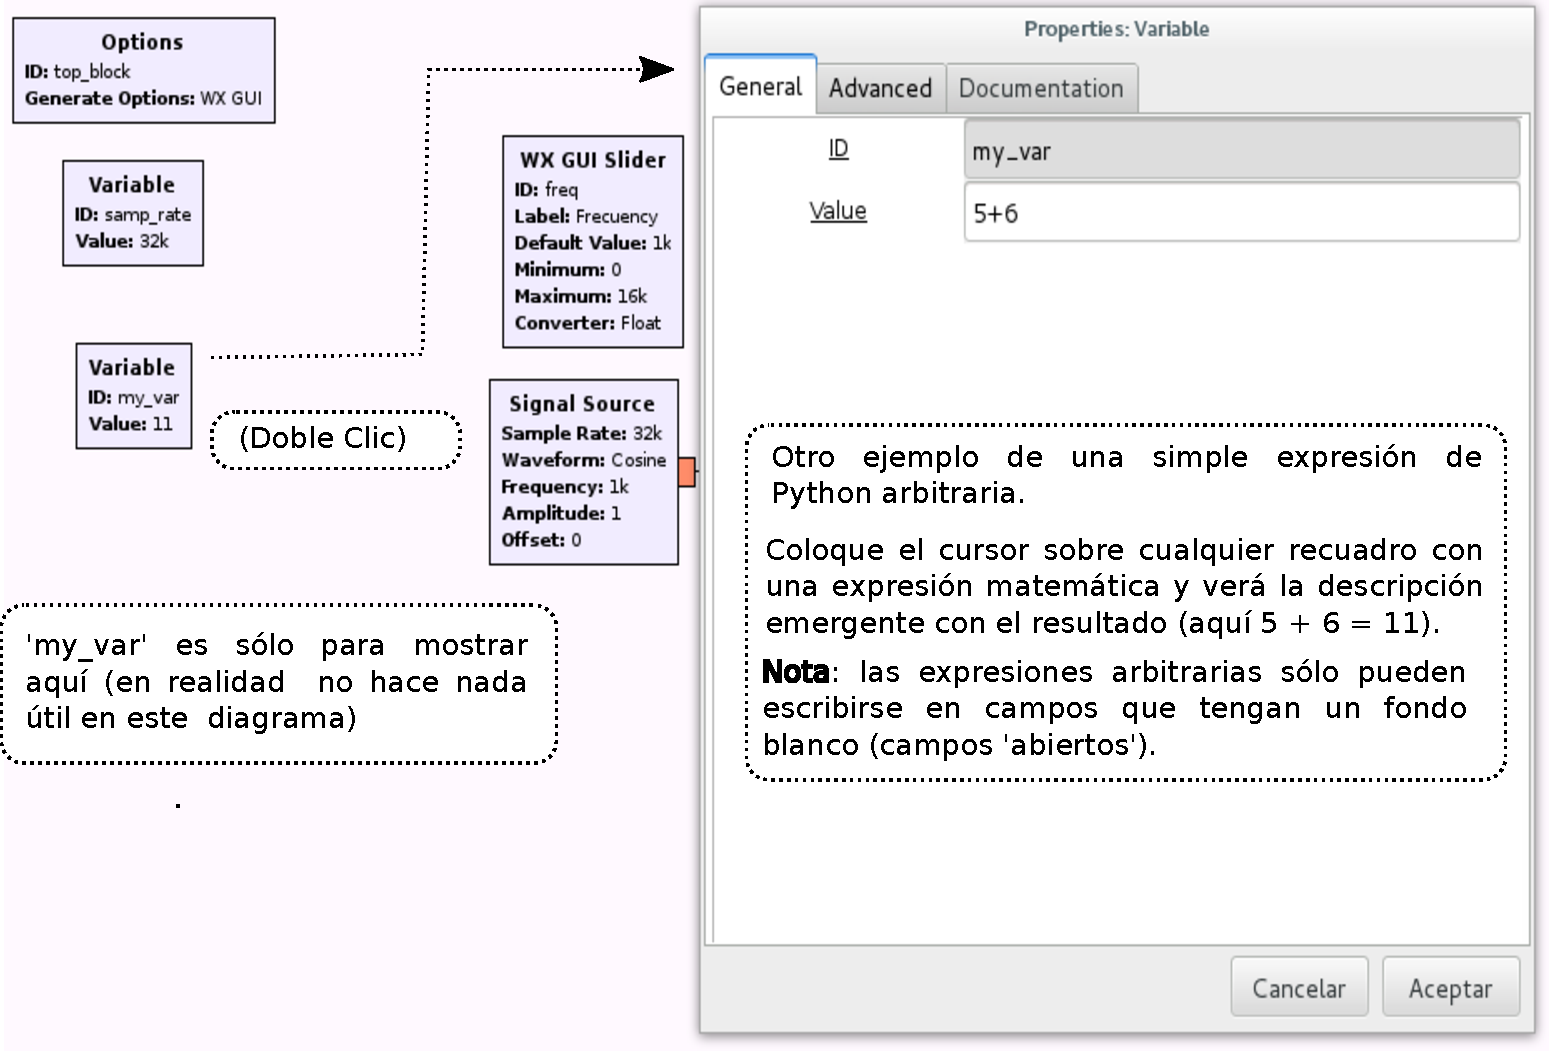
\includegraphics[width=.9\textwidth]{parte1/lab1/pdf/lab1_10.pdf}
\end{figure}
\end{frame}
%-----------------------------------

\begin{frame}{Primeros pasos }
\begin{figure}[H]
\vspace{-3mm}
\centering
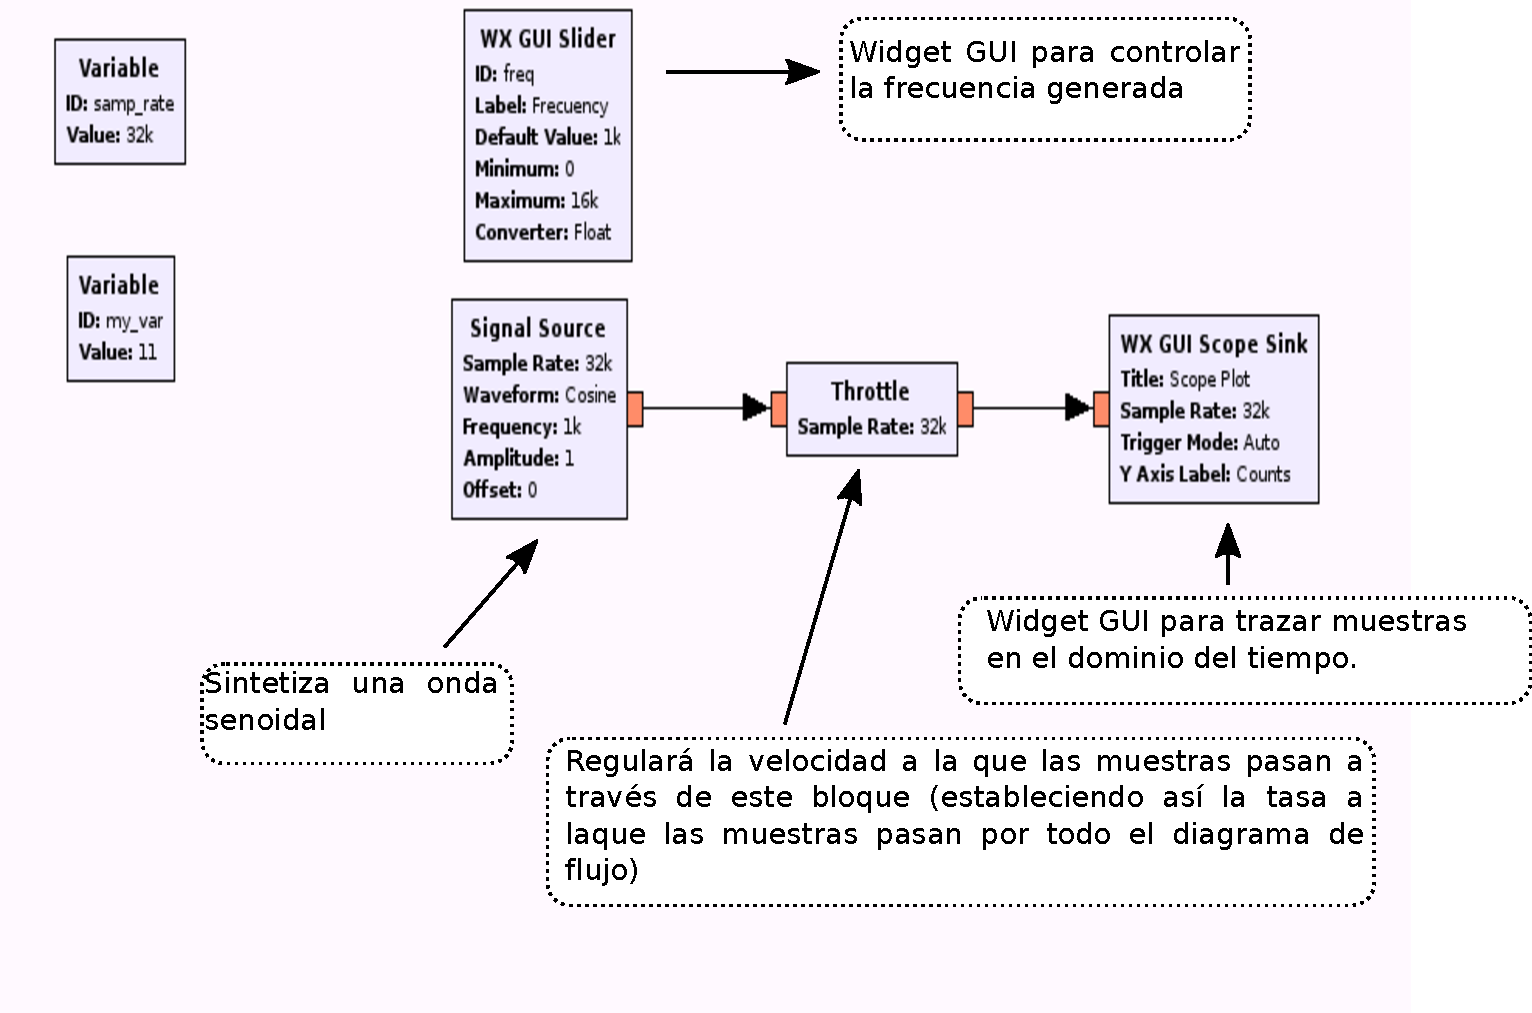
\includegraphics[width=\textwidth]{parte1/lab1/pdf/lab1_11.pdf}
\end{figure}
\end{frame}
%-----------------------------------

\begin{frame}{Primeros pasos }
\begin{figure}[H]
\vspace{-3mm}
\centering
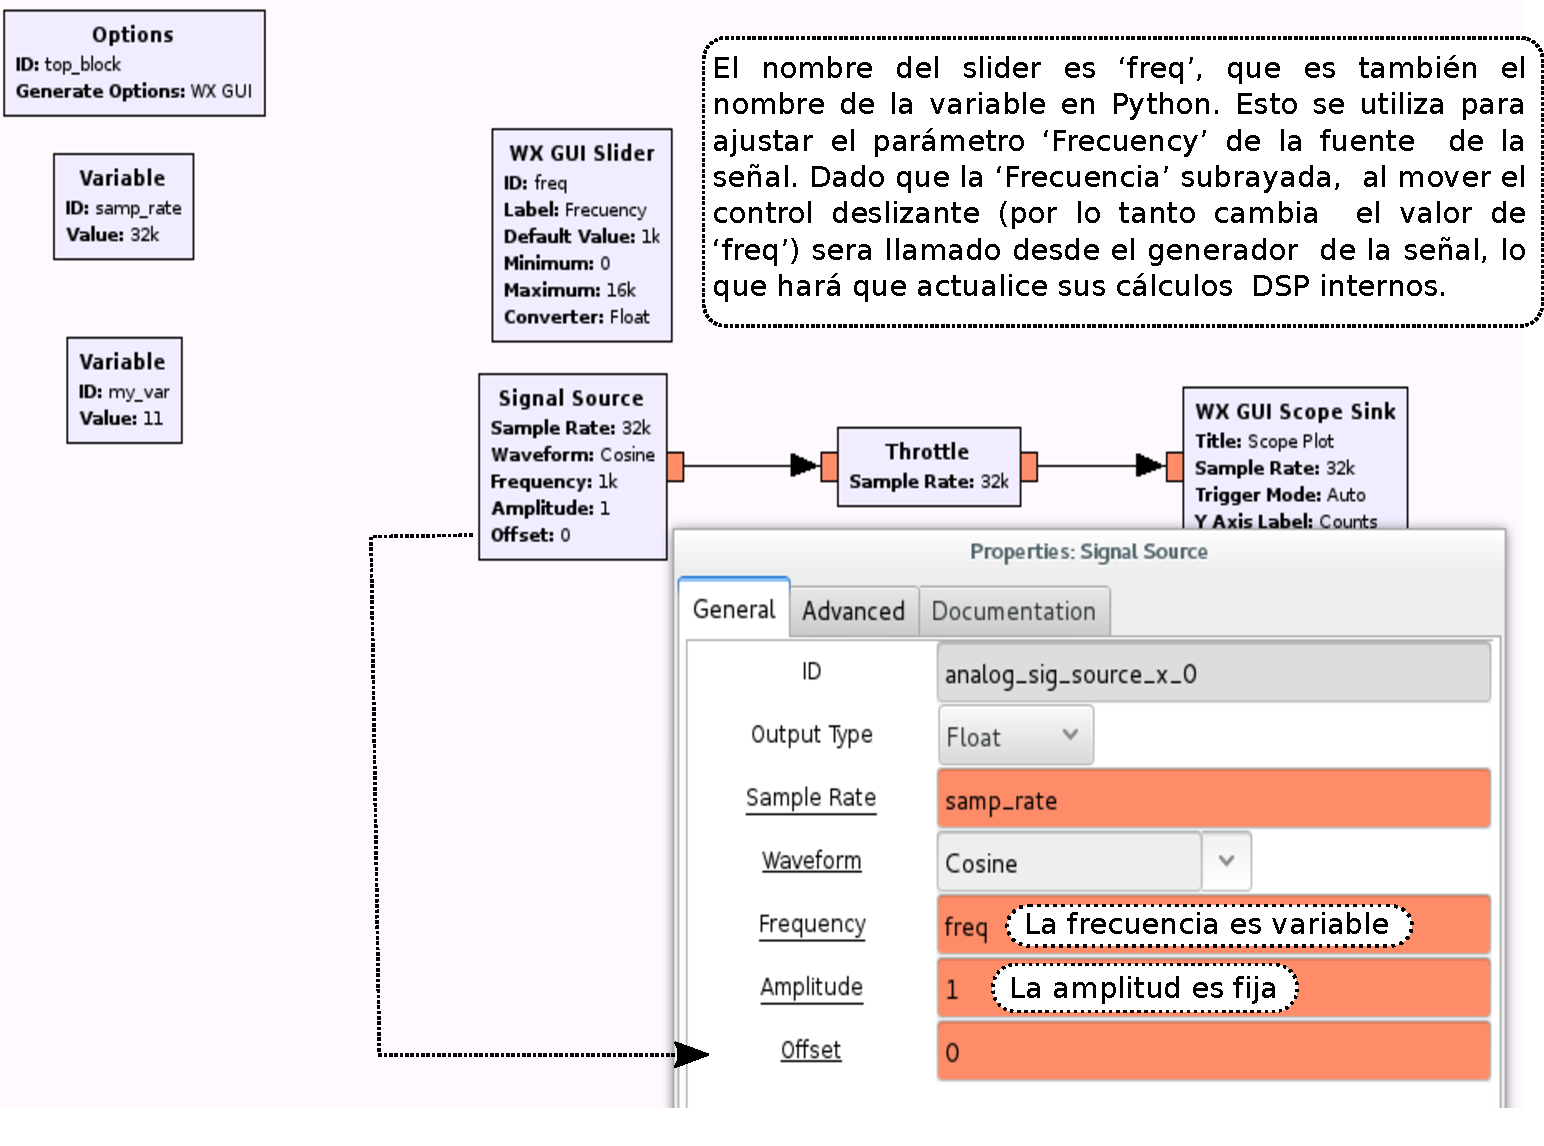
\includegraphics[width=.85\textwidth]{parte1/lab1/pdf/lab1_12.pdf}
\end{figure}
\end{frame}
%-----------------------------------

\begin{frame}{Primeros pasos }
\begin{figure}[H]
\vspace{-3mm}
\centering
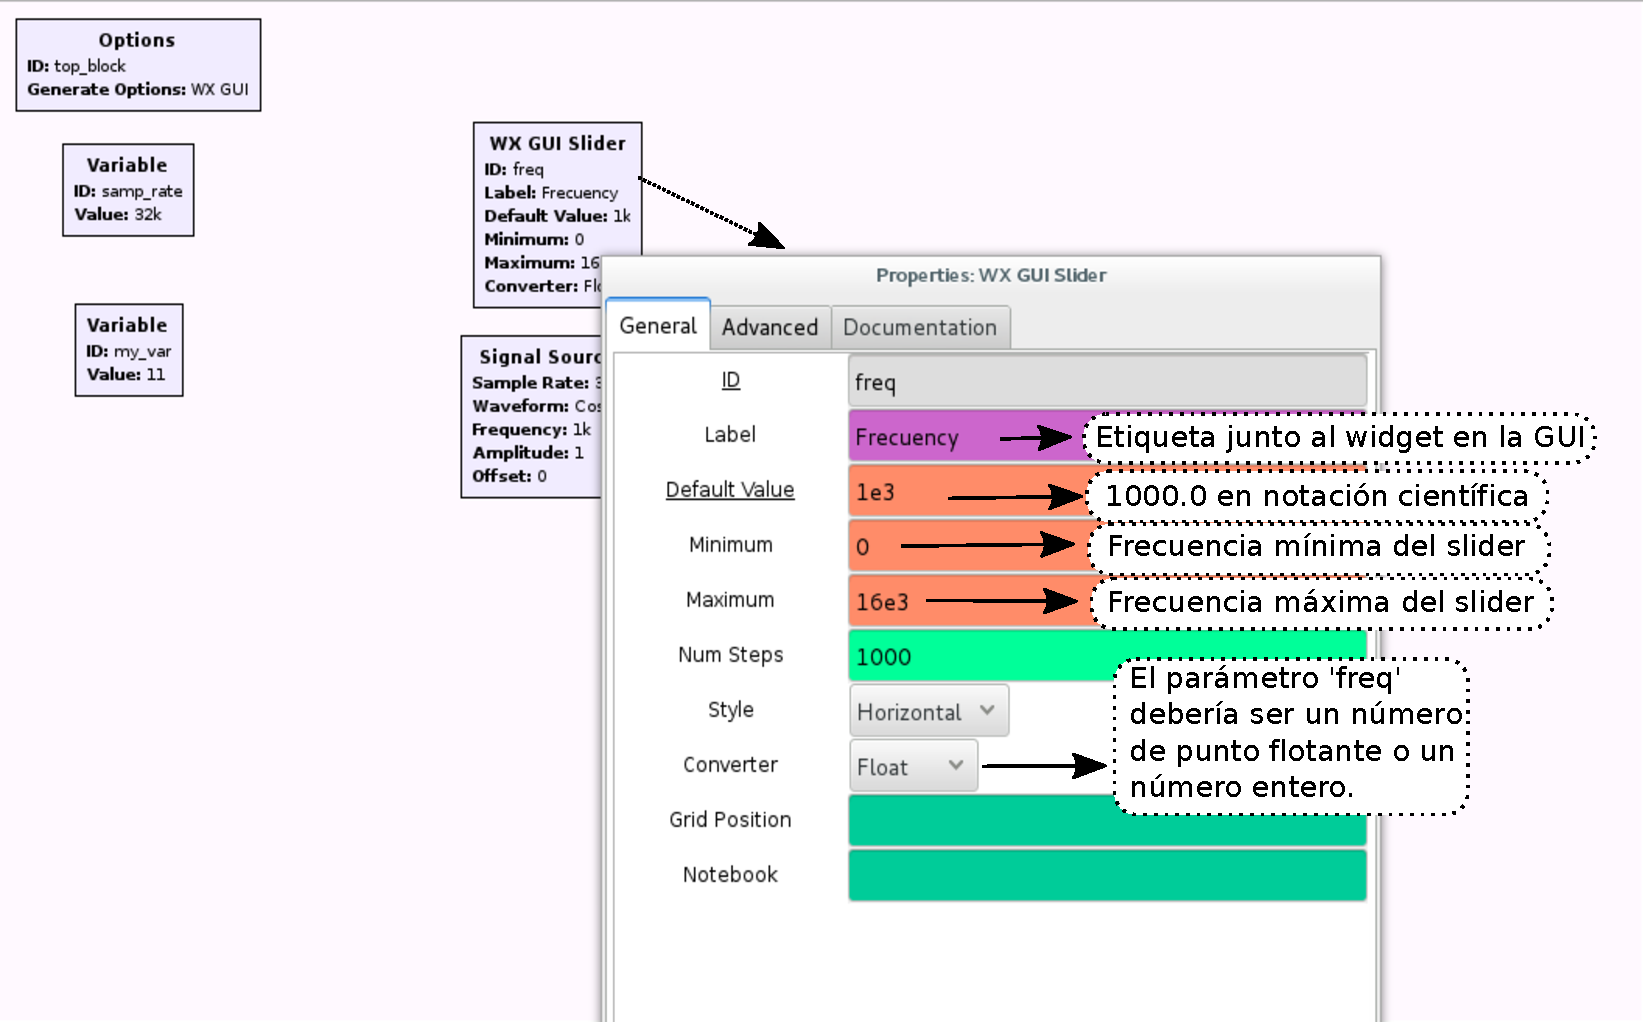
\includegraphics[width=\textwidth]{parte1/lab1/pdf/lab1_13.pdf}
\end{figure}
\end{frame}
%-----------------------------------

\begin{frame}{Primeros pasos }
\begin{figure}[H]
\vspace{-1cm}
\centering
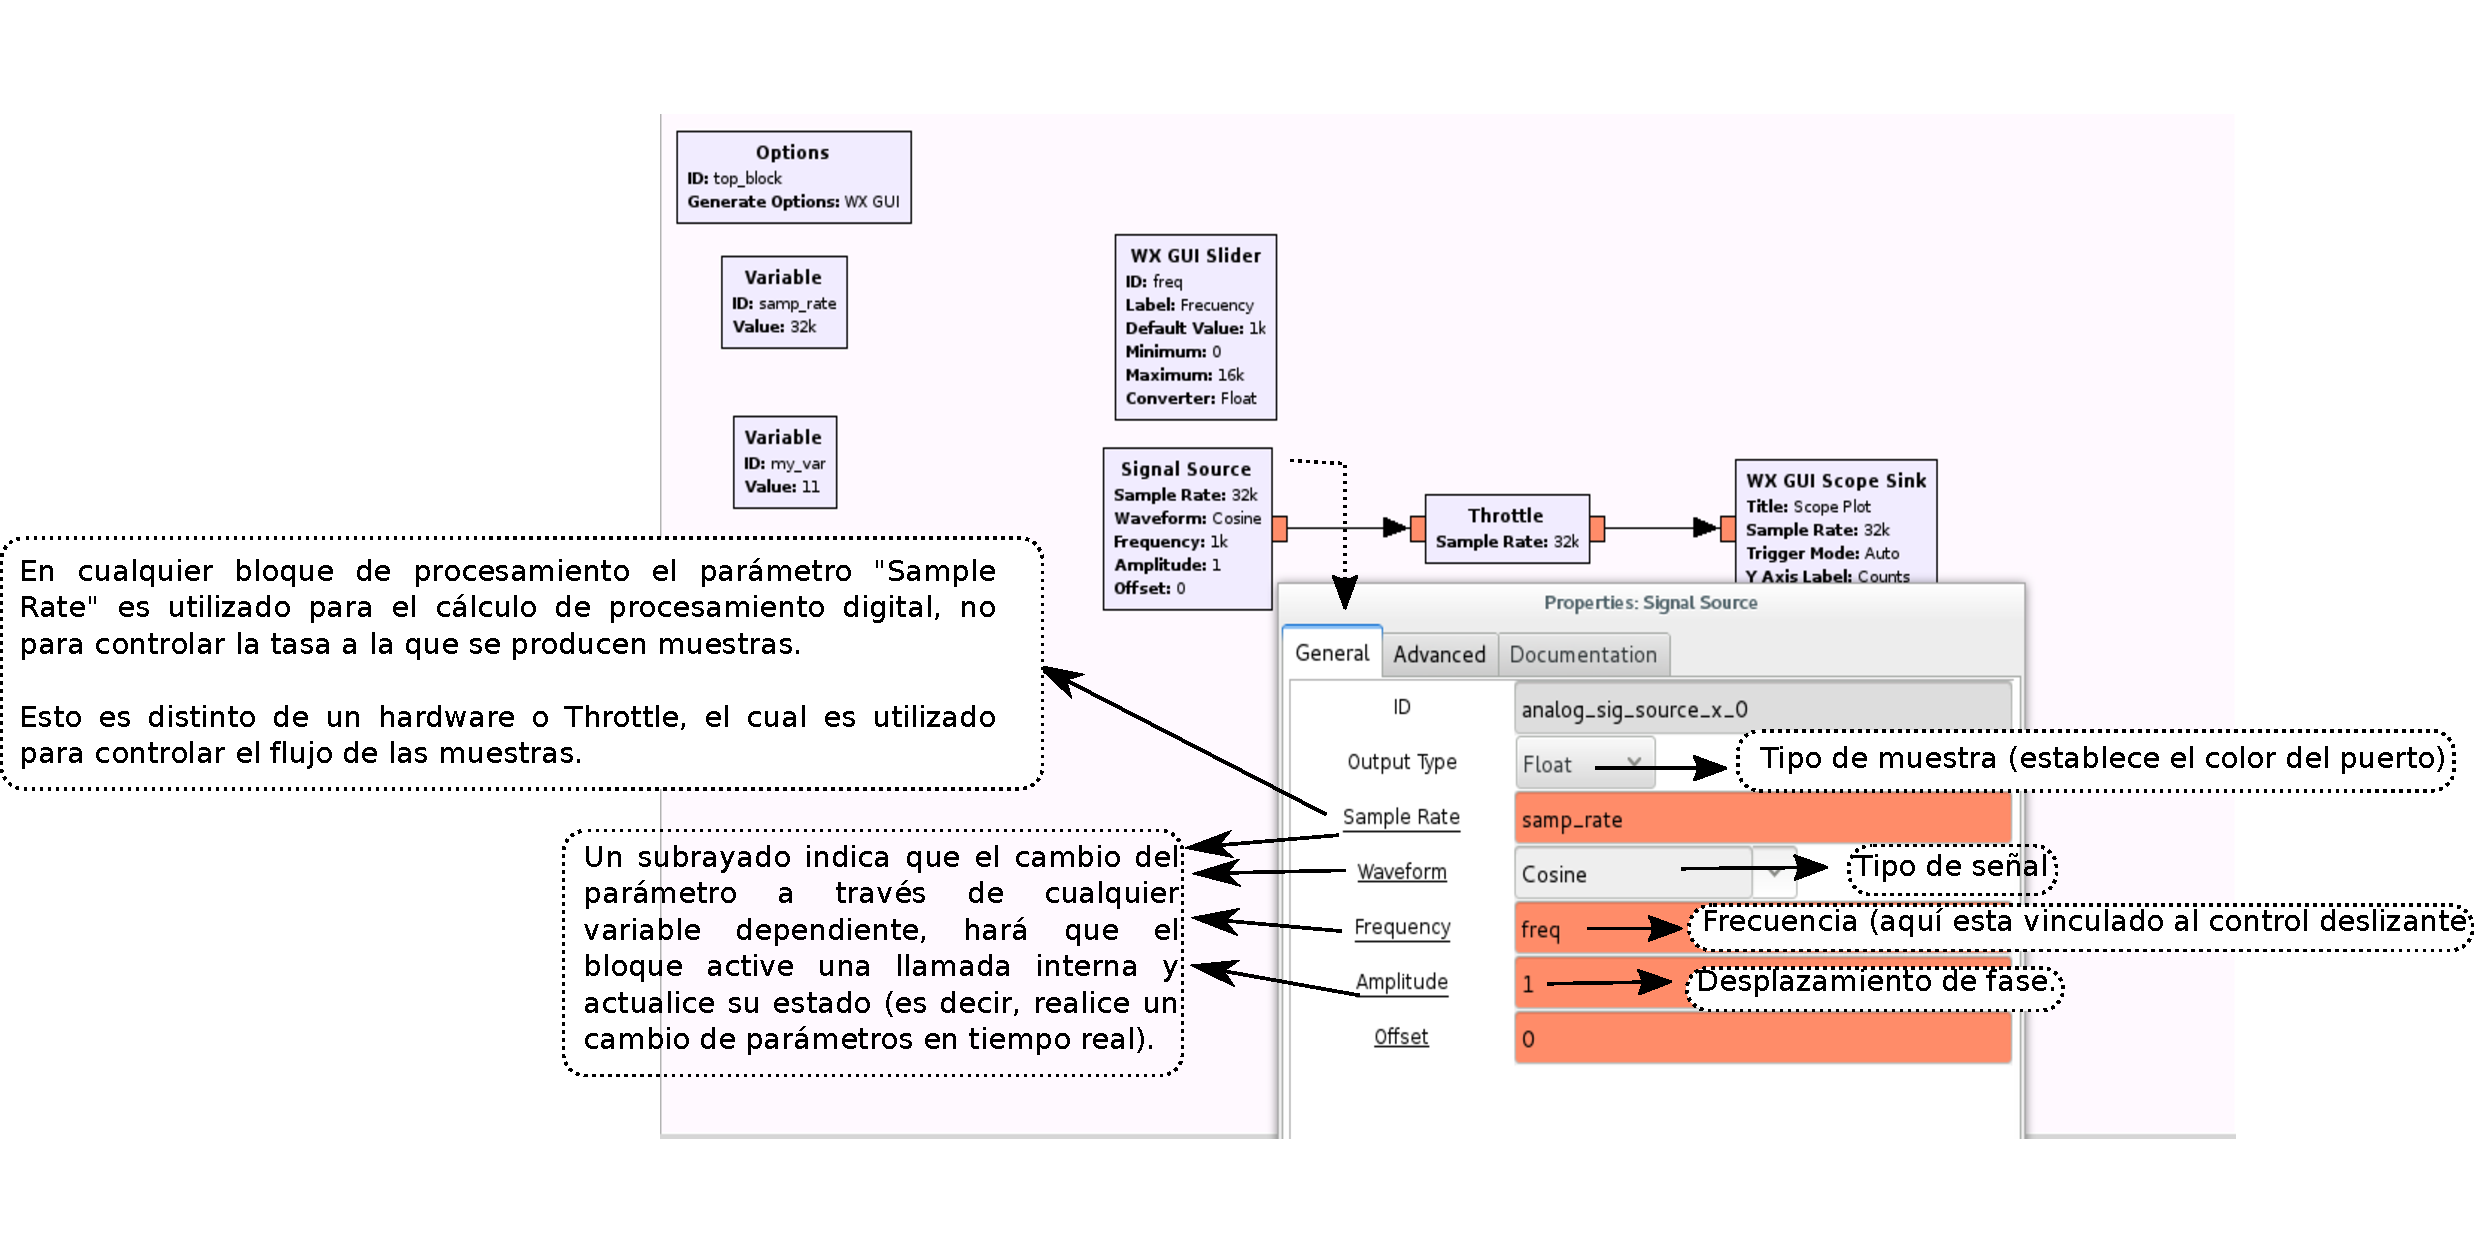
\includegraphics[width=1.05\textwidth]{parte1/lab1/pdf/lab1_14.pdf}
\end{figure}
\end{frame}
%-----------------------------------

\begin{frame}{Primeros pasos }
\begin{figure}[H]
\vspace{-3mm}
\centering
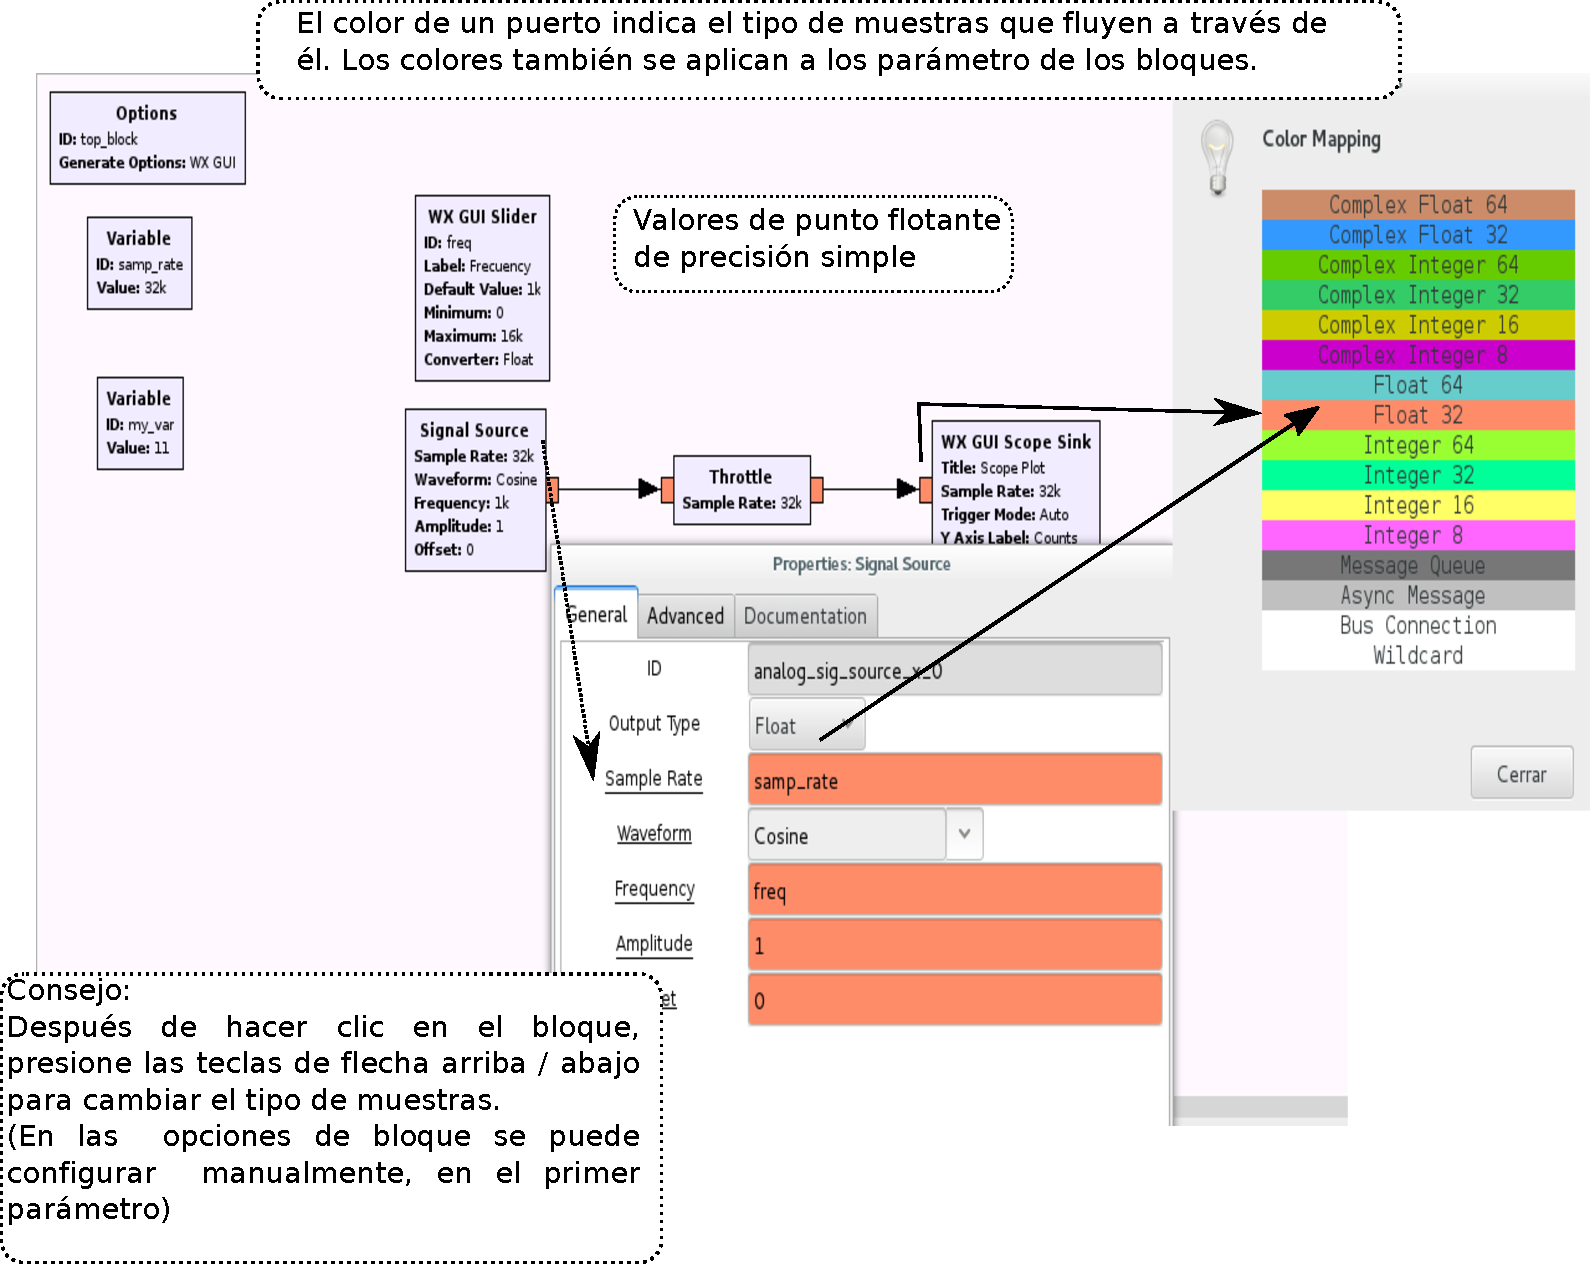
\includegraphics[width=.80\textwidth]{parte1/lab1/pdf/lab1_15.pdf}
\end{figure}
\end{frame}
%-----------------------------------

\begin{frame}{Primeros pasos }
\begin{figure}[H]
\centering
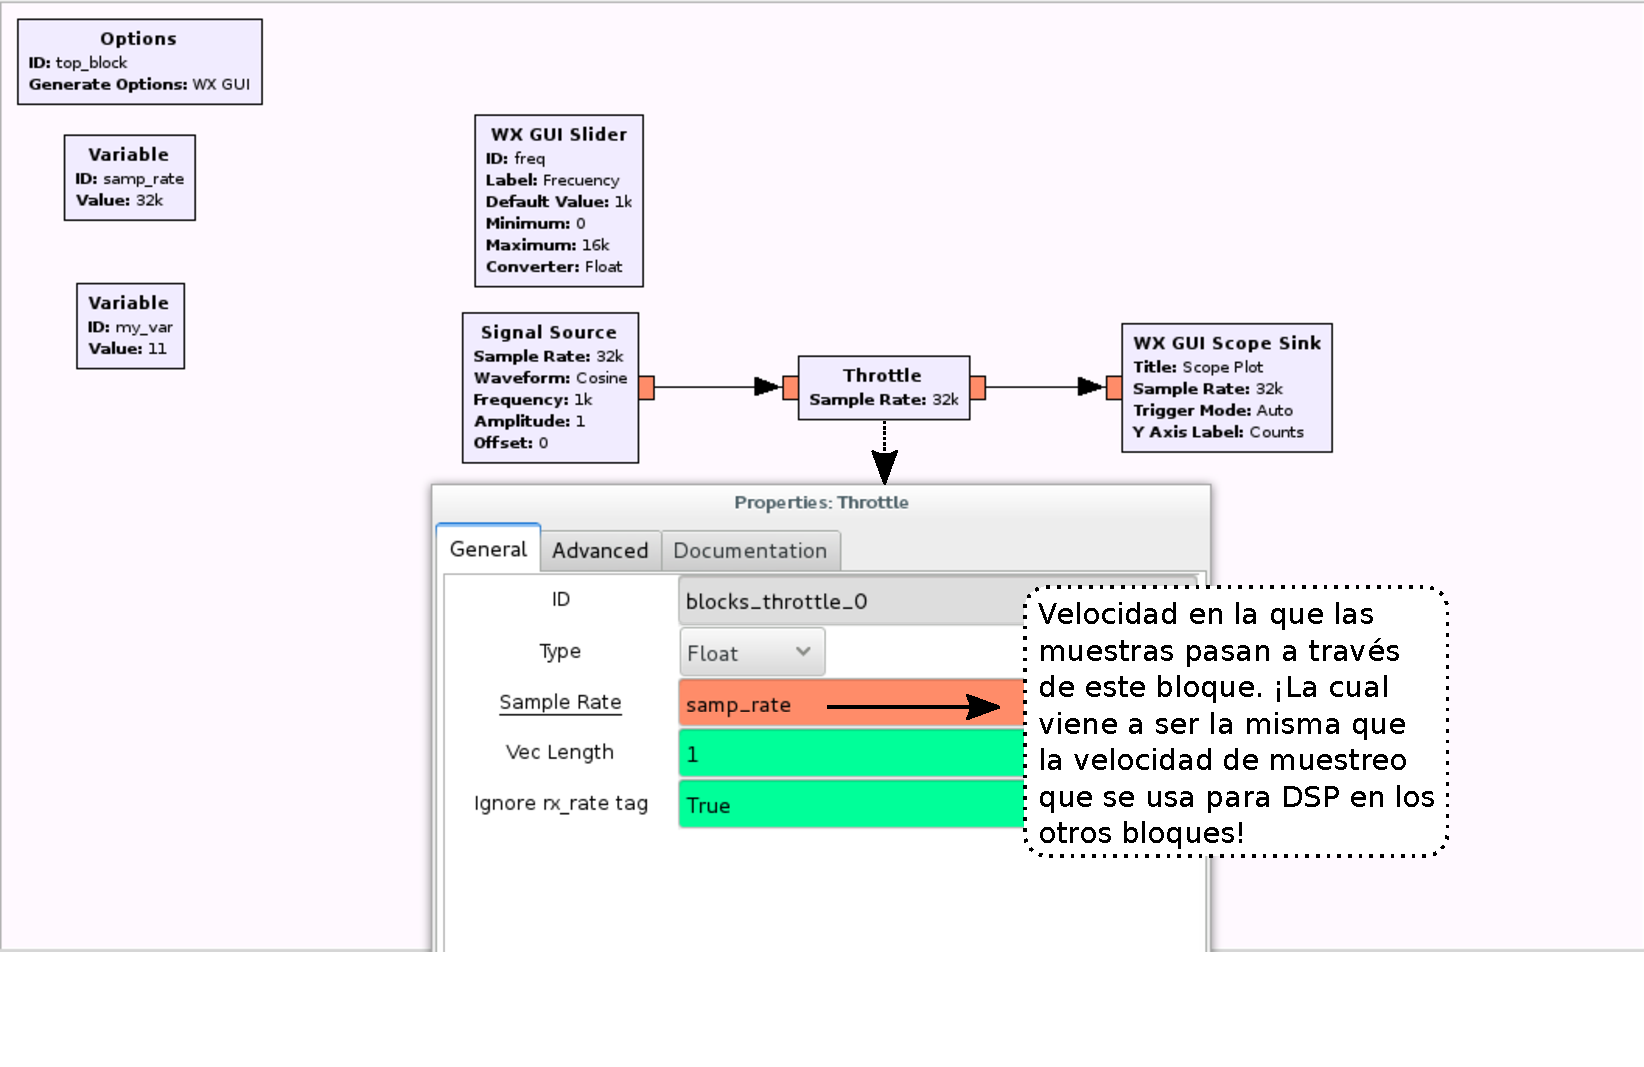
\includegraphics[width=\textwidth]{parte1/lab1/pdf/lab1_16.pdf}
\end{figure}
\end{frame}
%-----------------------------------

\begin{frame}{Primeros pasos }
\begin{figure}[H]
\vspace{-3mm}
\centering
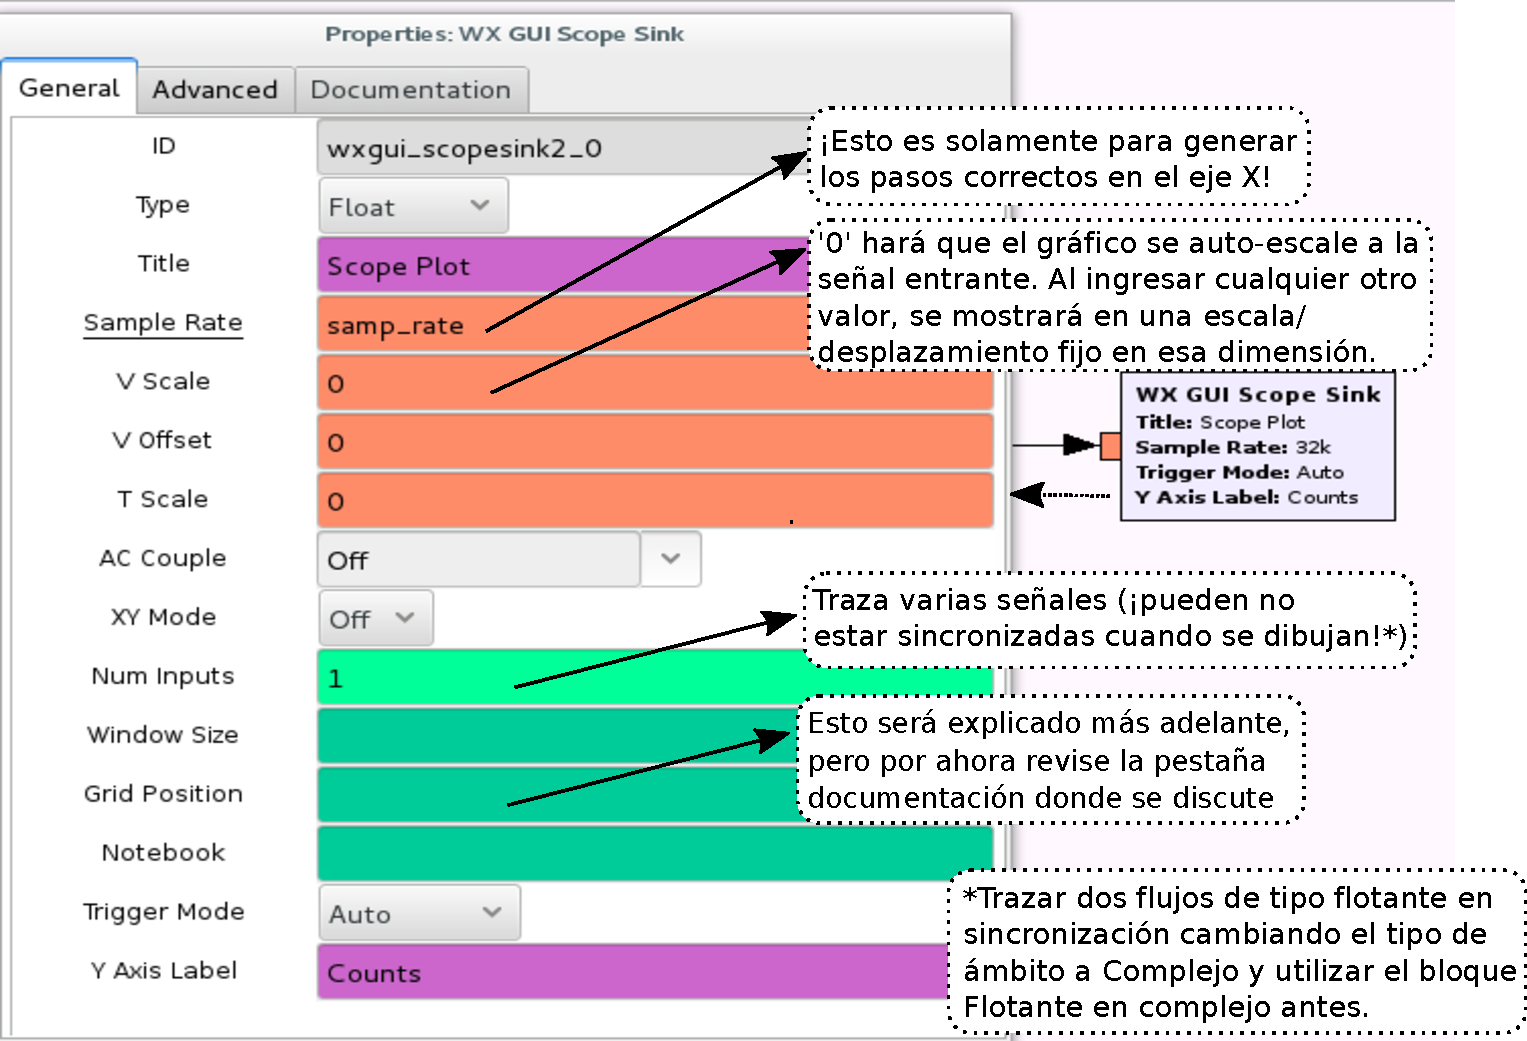
\includegraphics[width=.85\textwidth]{parte1/lab1/pdf/lab1_17.pdf}
\end{figure}
\end{frame}
%-----------------------------------

\begin{frame}{Primeros pasos }
\begin{figure}[H]
\centering
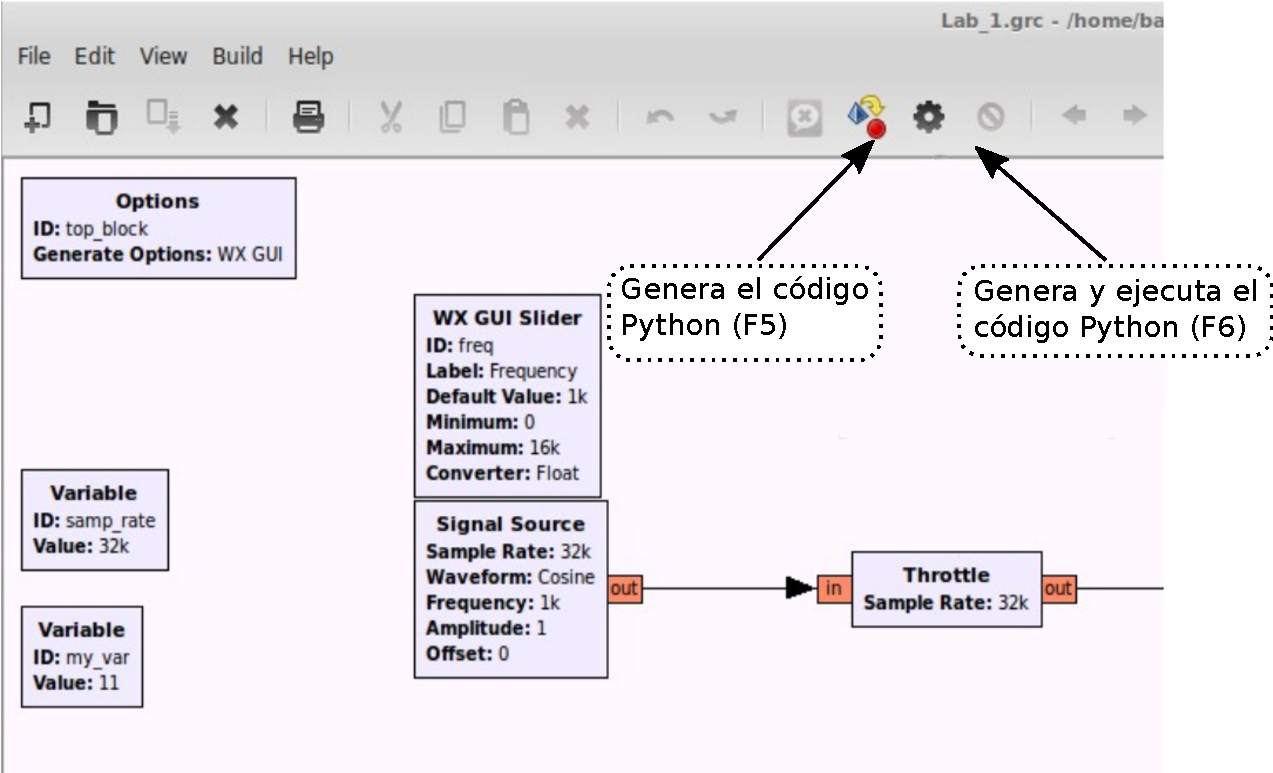
\includegraphics[width=\textwidth]{parte1/lab1/pdf/lab1_18.pdf}
\end{figure}
\end{frame}
%-----------------------------------

\begin{frame}{Primeros pasos }
\begin{figure}[H]
\centering
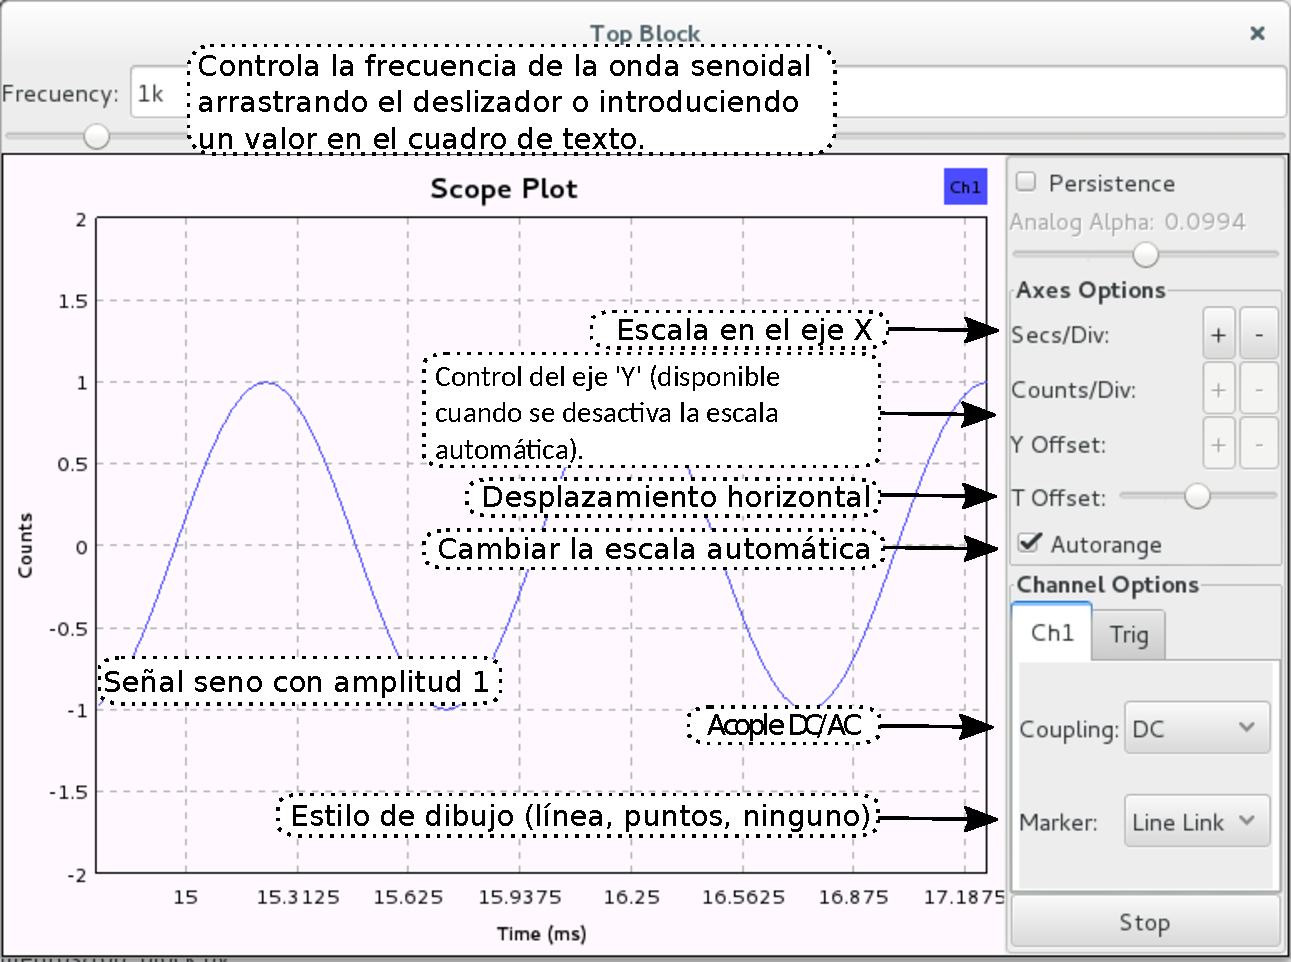
\includegraphics[width=\textwidth, height=0.55\textwidth]{parte1/lab1/pdf/lab1_19.pdf}
\end{figure}
\end{frame}
%-----------------------------------

\begin{frame}{Primeros pasos }
\begin{figure}[H]
\centering
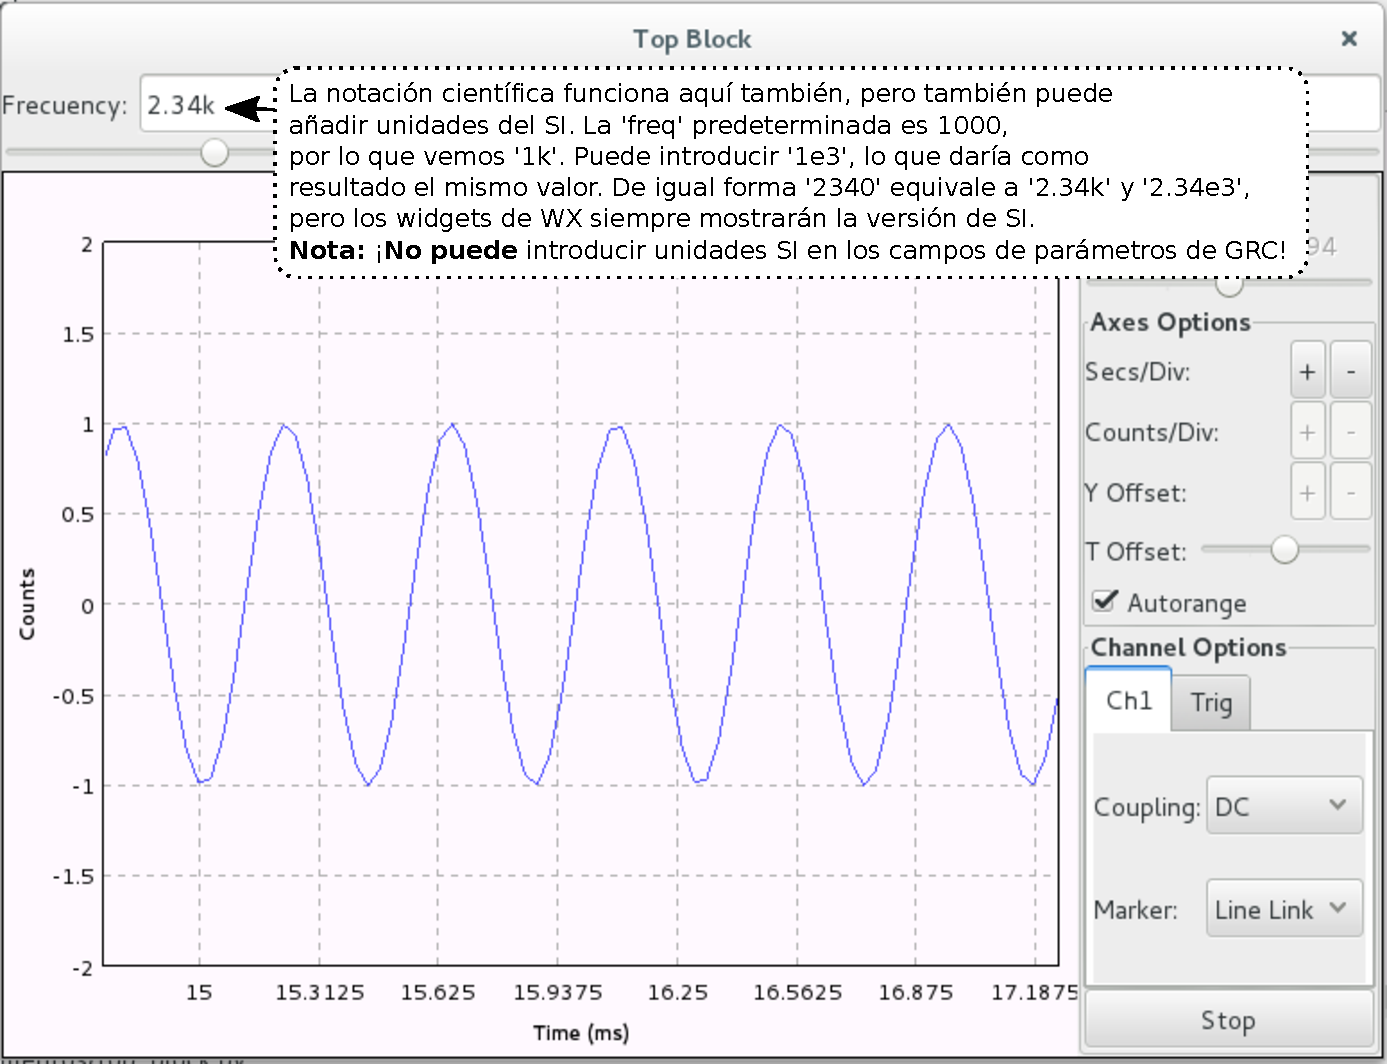
\includegraphics[width=\textwidth, height=0.55\textwidth]{parte1/lab1/pdf/lab1_20.pdf}
\end{figure}
\end{frame}
%-----------------------------------

\begin{frame}{Primeros pasos }
\begin{figure}[H]
\centering
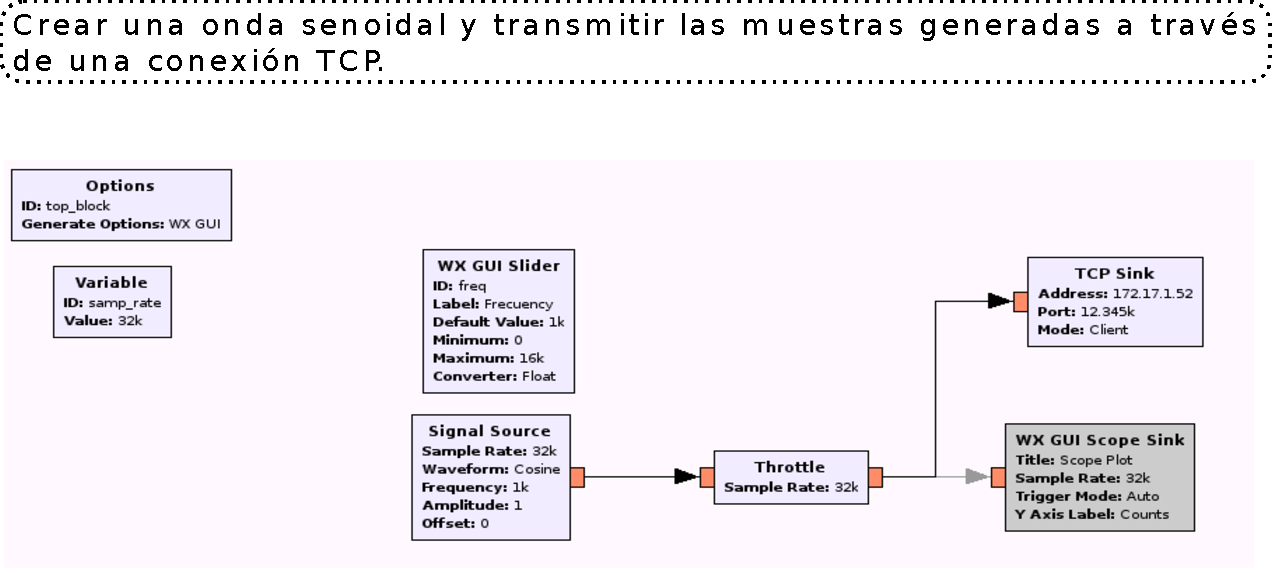
\includegraphics[width=\textwidth]{parte1/lab1/pdf/lab1_21.pdf}
\end{figure}
\end{frame}
%-----------------------------------

\begin{frame}{Primeros pasos }
\begin{figure}[H]
\centering
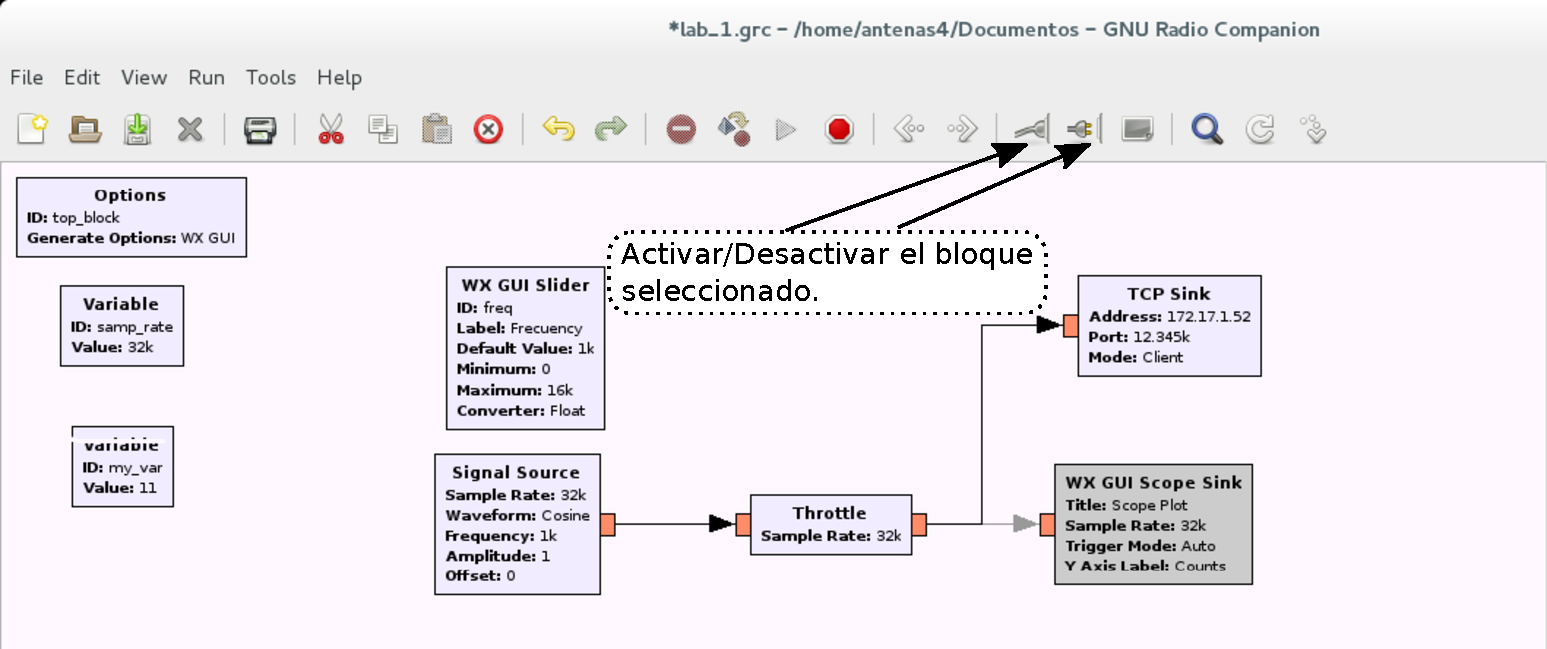
\includegraphics[width=\textwidth]{parte1/lab1/pdf/lab1_22.pdf}
\end{figure}
\end{frame}
%-----------------------------------

\begin{frame}{Primeros pasos }
\begin{figure}[H]
\centering
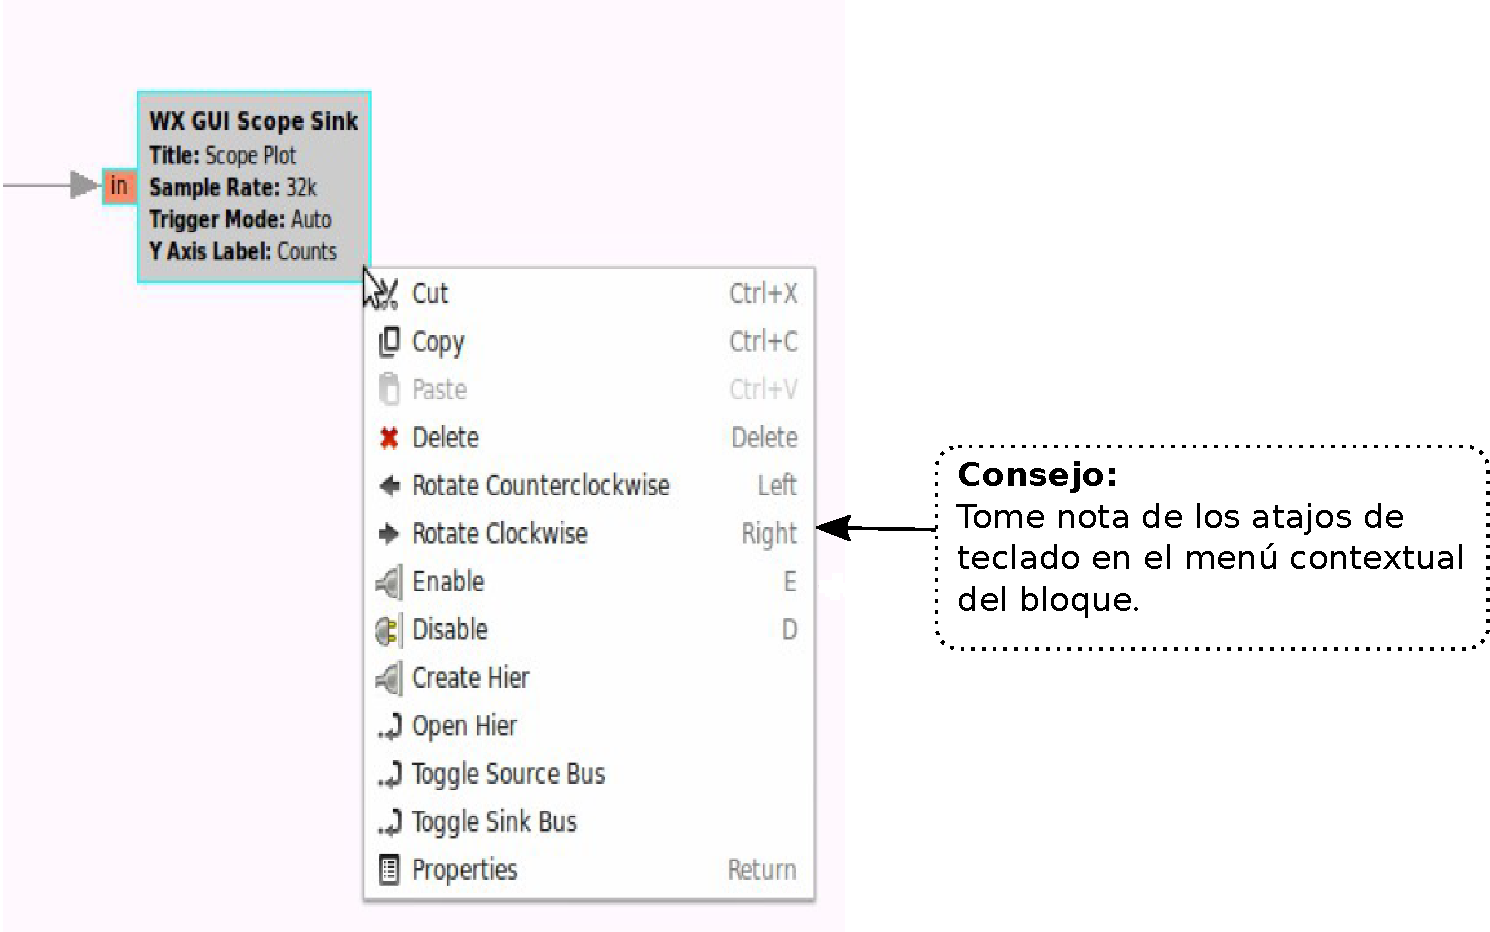
\includegraphics[width=\textwidth, height=0.6\textwidth]{parte1/lab1/pdf/lab1_23.pdf}
\end{figure}
\end{frame}
%-----------------------------------

\begin{frame}{Primeros pasos }
\begin{figure}[H]
\centering
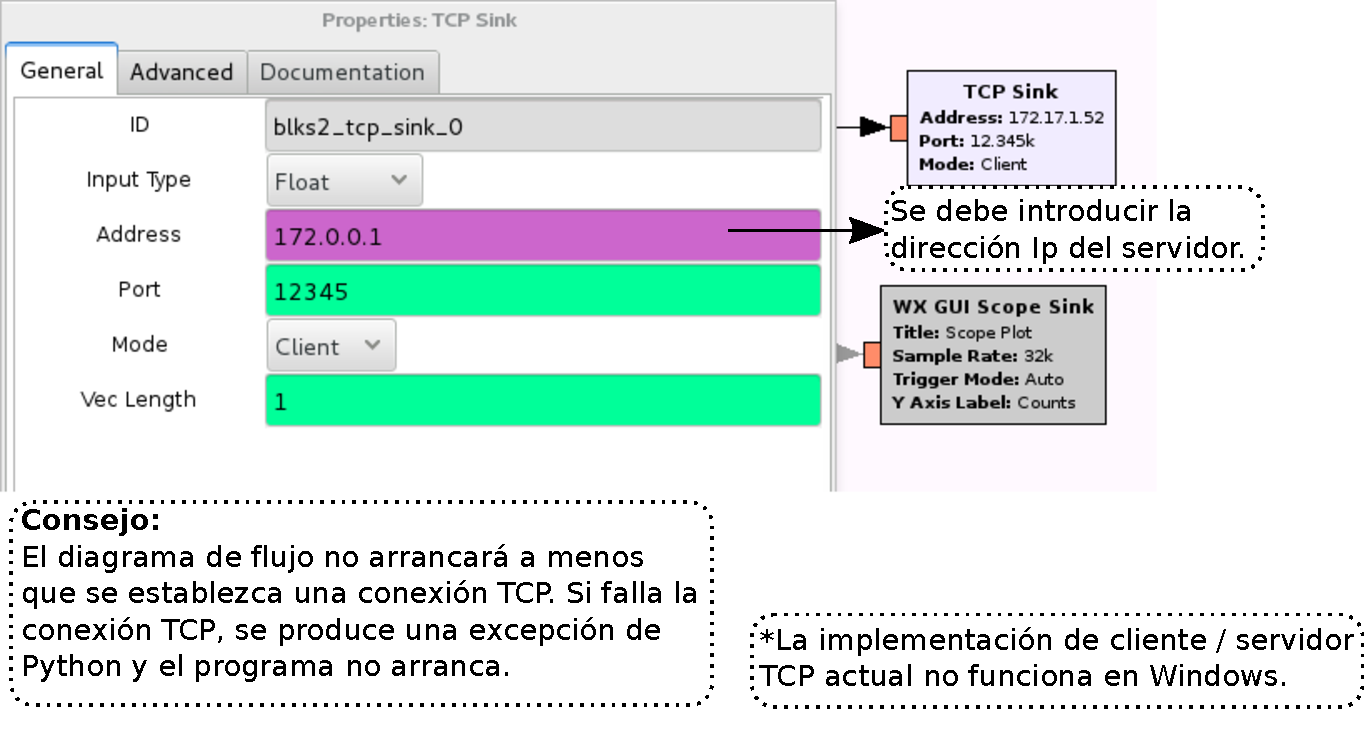
\includegraphics[width=\textwidth]{parte1/lab1/pdf/lab1_24.pdf}
\end{figure}
\end{frame}
%-----------------------------------

\begin{frame}{Primeros pasos }
\begin{figure}[H]
\centering
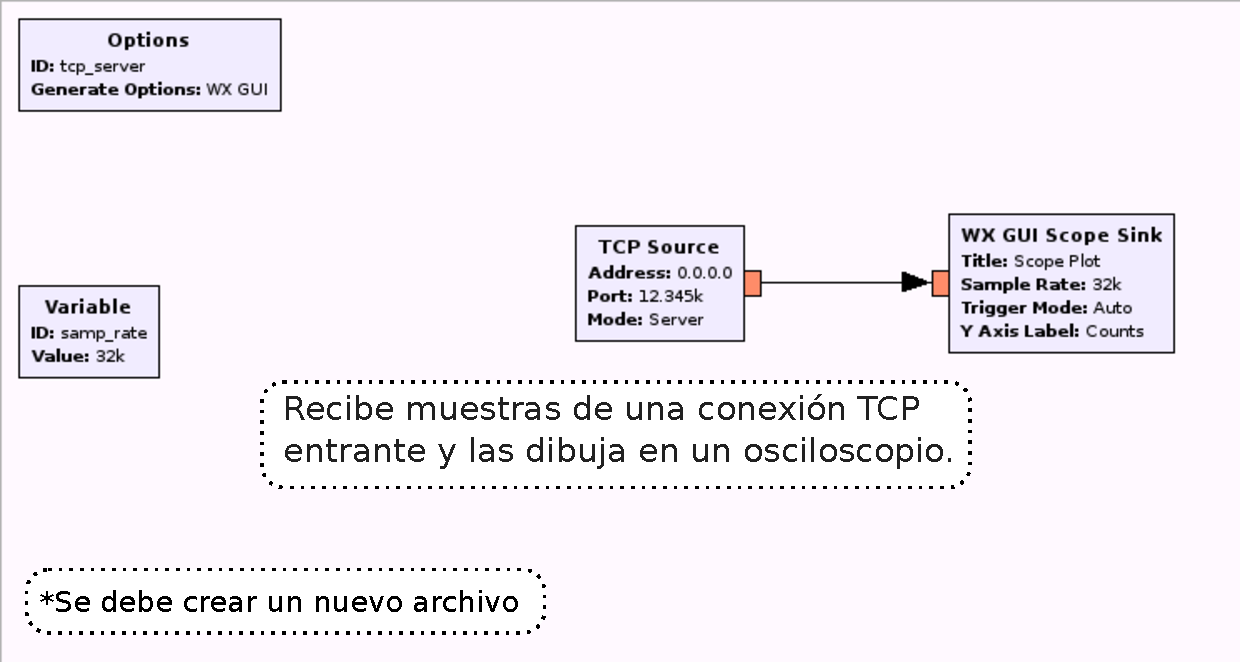
\includegraphics[width=\textwidth]{parte1/lab1/pdf/lab1_25.pdf}
\end{figure}
\end{frame}
%-----------------------------------

\begin{frame}{Primeros pasos }
\begin{figure}[H]
\centering
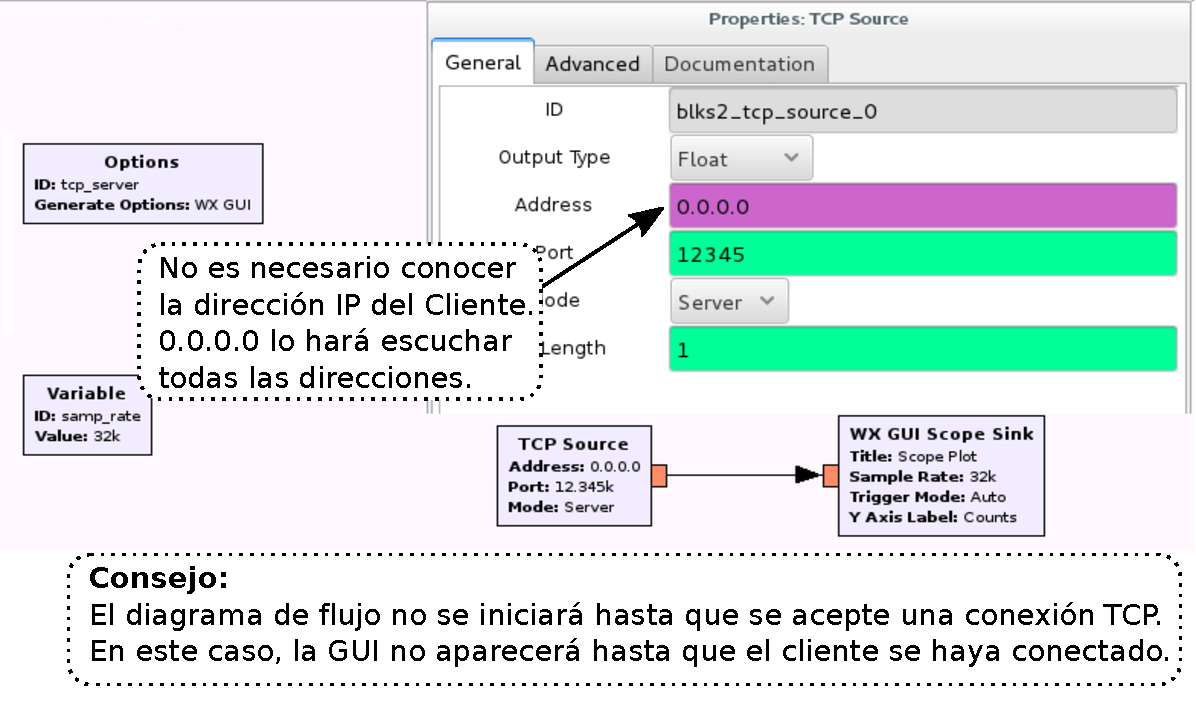
\includegraphics[width=\textwidth]{parte1/lab1/pdf/lab1_26.pdf}
\end{figure}
\end{frame}
%-----------------------------------

\begin{frame}{Primeros pasos }
\begin{figure}[H]
\centering
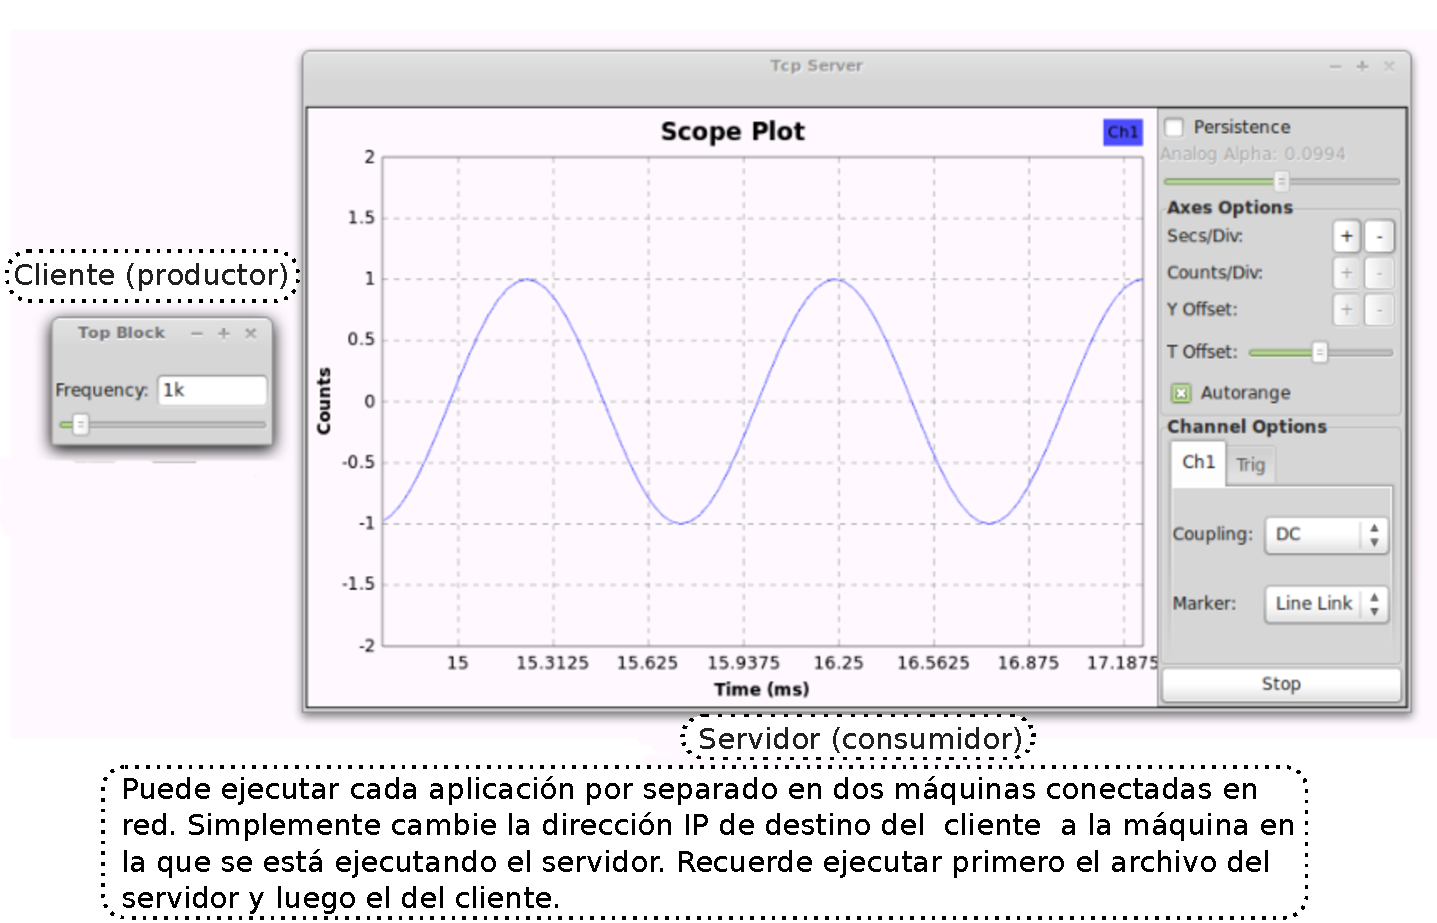
\includegraphics[width=\textwidth, height=0.55\textwidth]{parte1/lab1/pdf/lab1_27.pdf}
\end{figure}
\end{frame}
%-----------------------------------

%///////////////////////////////////////////////////////////////

\subsection{Lab2: Osciloscopio y FFT}
%*********************
\begin{frame}{}

\pgfdeclareimage[width=\paperwidth,height=\paperheight]{bg}{imagenes/fondo_lab}
\setbeamertemplate{background}{\pgfuseimage{bg}}

\bfseries{\textrm{\LARGE Lab2\\ \Large Osciloscopio y FFT}}
\raggedright
\end{frame}
%*********************

%-----------------------------------
\begin{frame}{Osciloscopio y FFT\index{TCP}}

\pgfdeclareimage[width=\paperwidth,height=\paperheight]{bg}{imagenes/fondo3}
\setbeamertemplate{background}{\pgfuseimage{bg}}

En este laboratorio se genera una onda senoidal y a su vez algún ruido; estas dos señales se suman y se observa el resultado en el dominio de la frecuencia (FFT) y del tiempo (Scope). Se aprende a utilizar el notebook y algunas herramientas básicas del GRC. 

\end{frame}
%---------------------------------

\begin{frame}{Osciloscopio y FFT\index{TCP}}

\begin{figure}[H]
\vspace{-4mm}
\centering
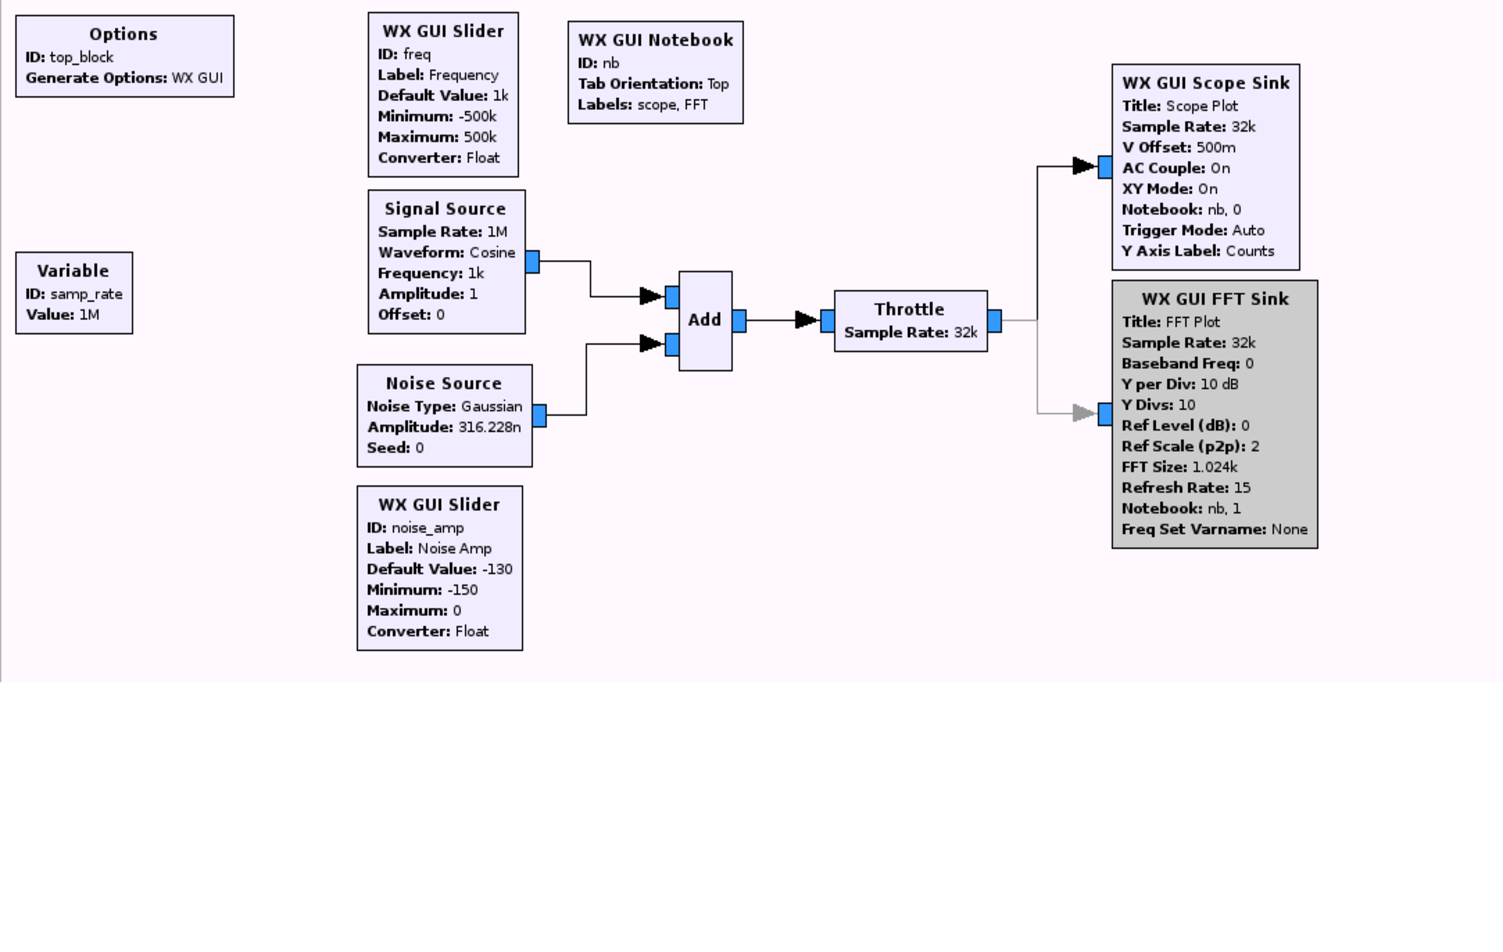
\includegraphics[width=1.2\textwidth]{parte1/lab2/pdf/lab2_1.pdf}
\end{figure}
\end{frame}
%---------------------------------

\begin{frame}{Osciloscopio y FFT}
\begin{figure}[H]
\vspace{-4mm}
\centering
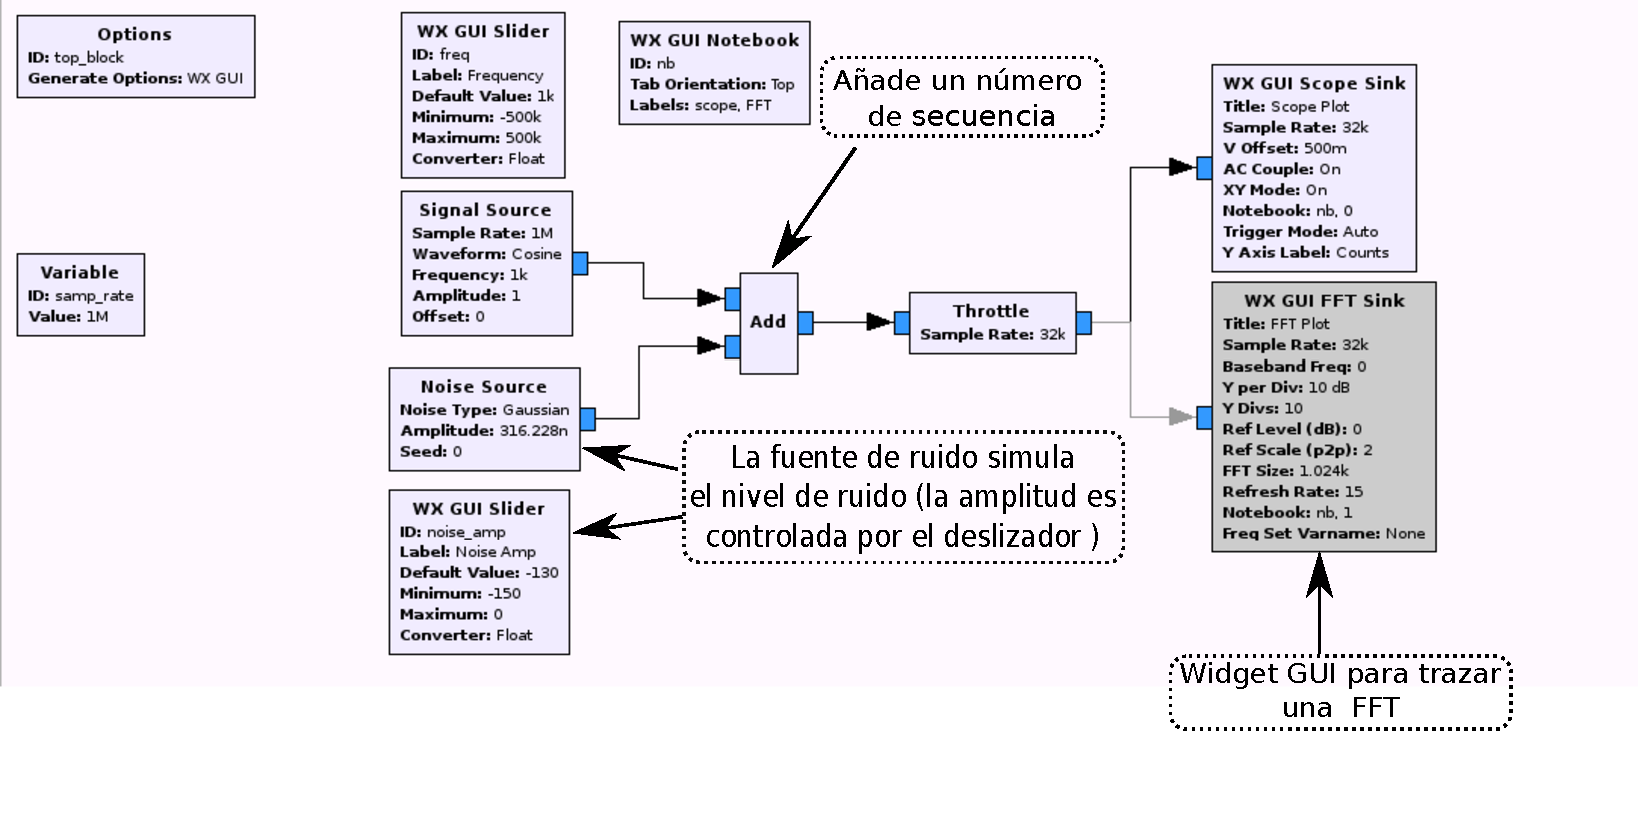
\includegraphics[width=1.1\textwidth]{parte1/lab2/pdf/lab2_2.pdf}
\end{figure}
\end{frame}
%--------------------------------

\begin{frame}{Osciloscopio y FFT\index{Noise Source}}
\begin{figure}[H]
\centering
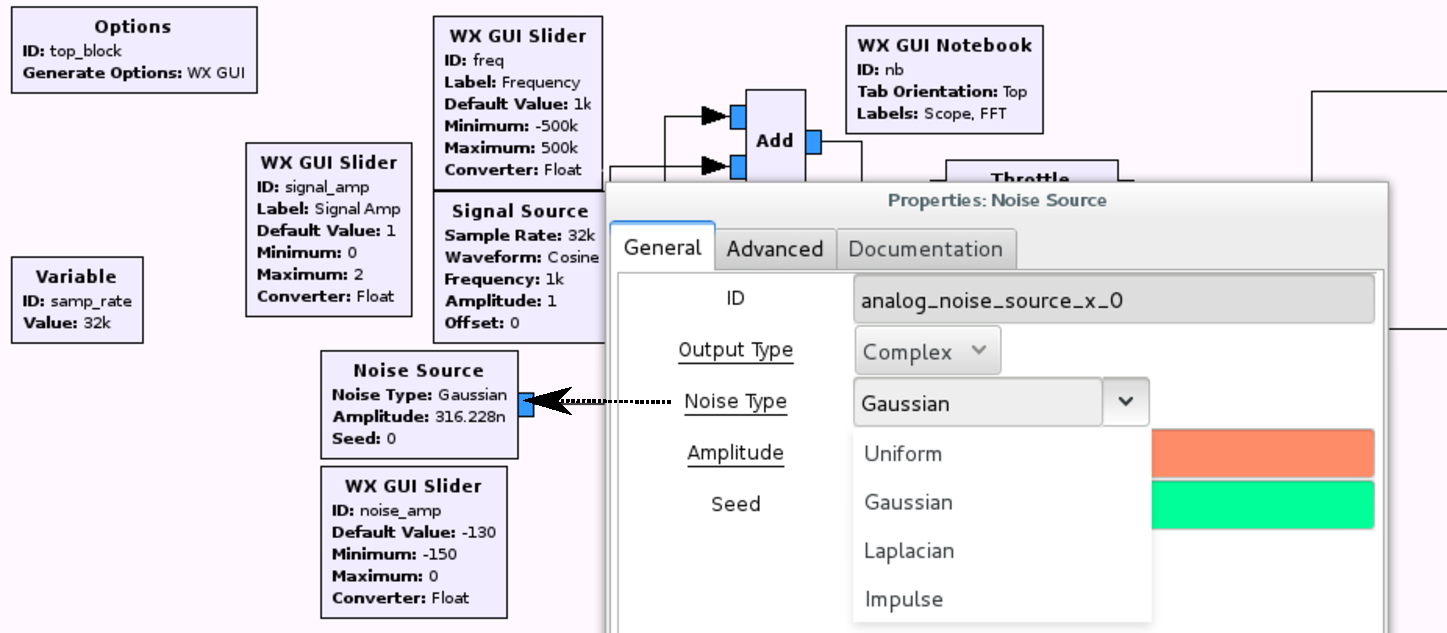
\includegraphics[width=1.055\textwidth]{parte1/lab2/pdf/lab2_3.pdf}
\end{figure}
\end{frame}
%--------------------------------

\begin{frame}{Osciloscopio y FFT\index{Noise Source}}
\begin{figure}[H]
\centering
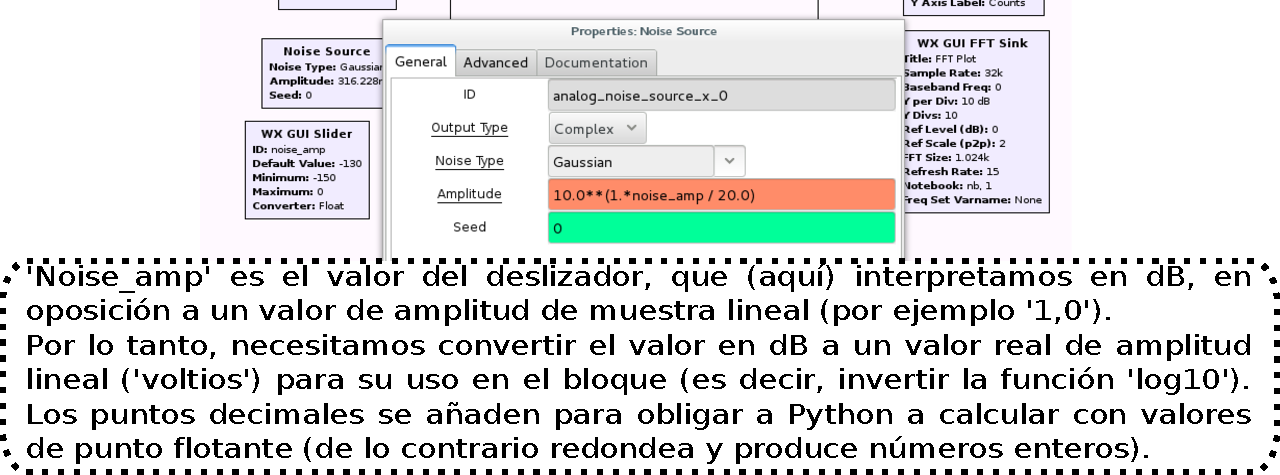
\includegraphics[width=1.055\textwidth]{parte1/lab2/pdf/lab2_4.pdf}
\end{figure}
\end{frame}
%--------------------------------

\begin{frame}{Osciloscopio y FFT\index{Add}}
\begin{figure}[H]
\centering
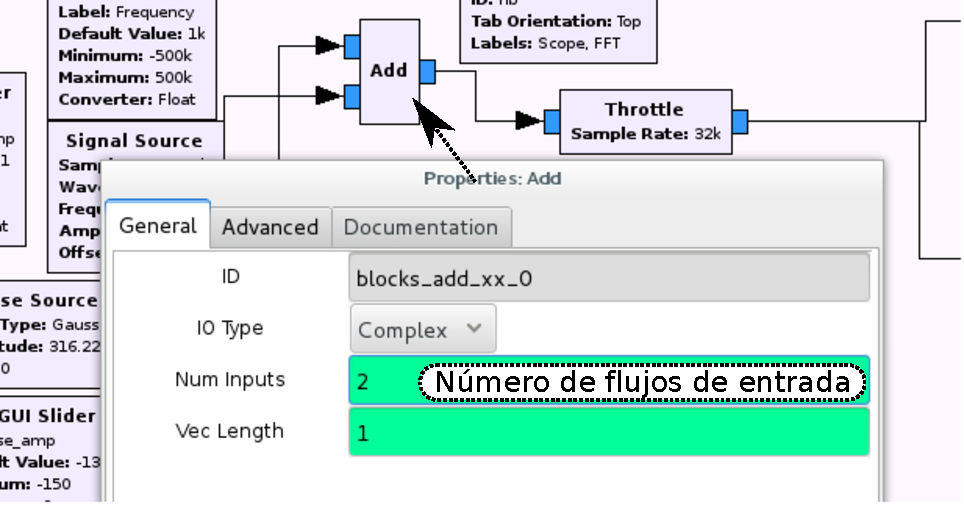
\includegraphics[width=.7\textwidth]{parte1/lab2/pdf/lab2_5.pdf}
\end{figure}
\end{frame}
%--------------------------------

\begin{frame}{Osciloscopio y FFT}
\begin{figure}[H]
\vspace{-4mm}
\centering
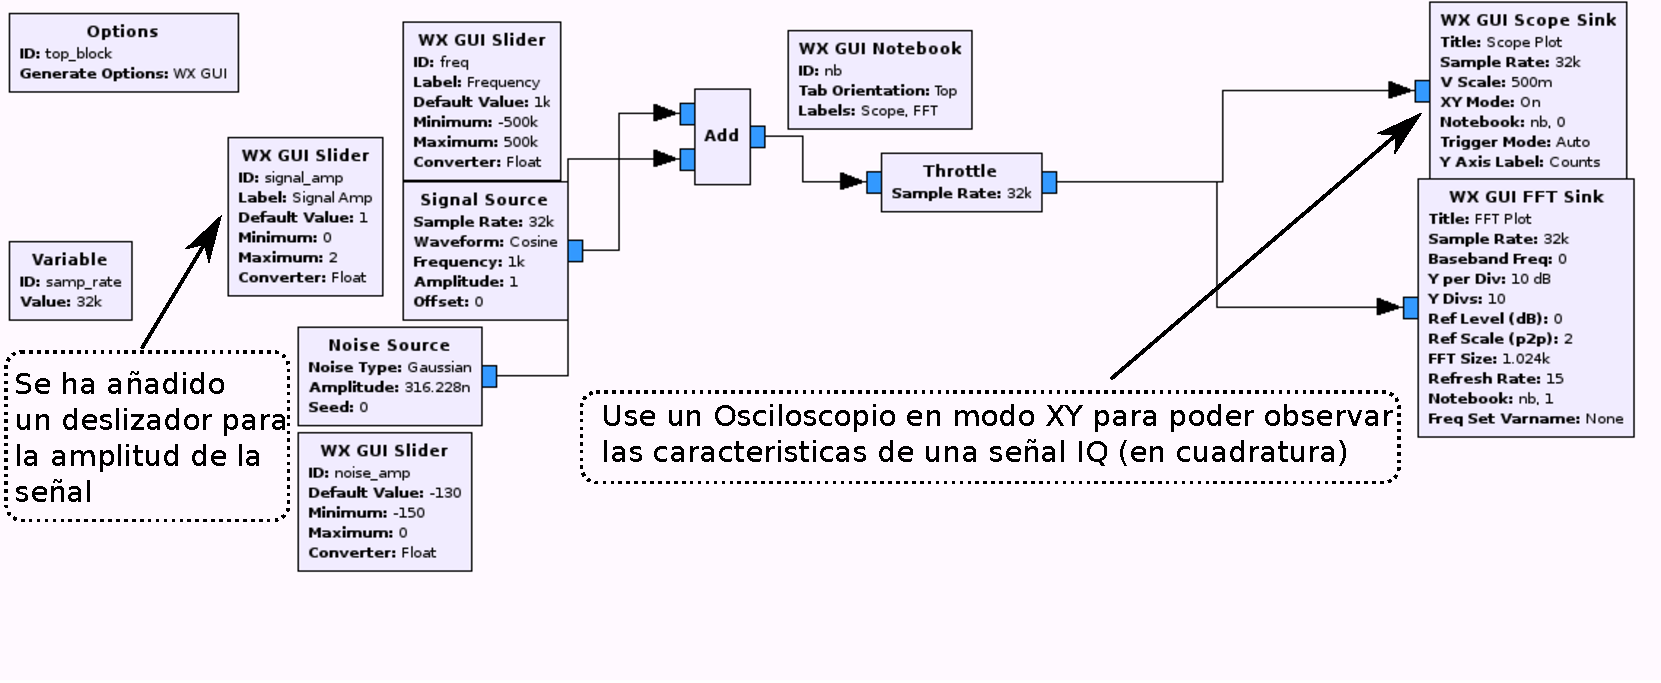
\includegraphics[width=1.1\textwidth]{parte1/lab2/pdf/lab2_6.pdf}
\end{figure}
\end{frame}
%--------------------------------

\begin{frame}{Osciloscopio y FFT\index{WX GUI Notebook}}
\begin{figure}[H]
\vspace{-4mm}
\centering
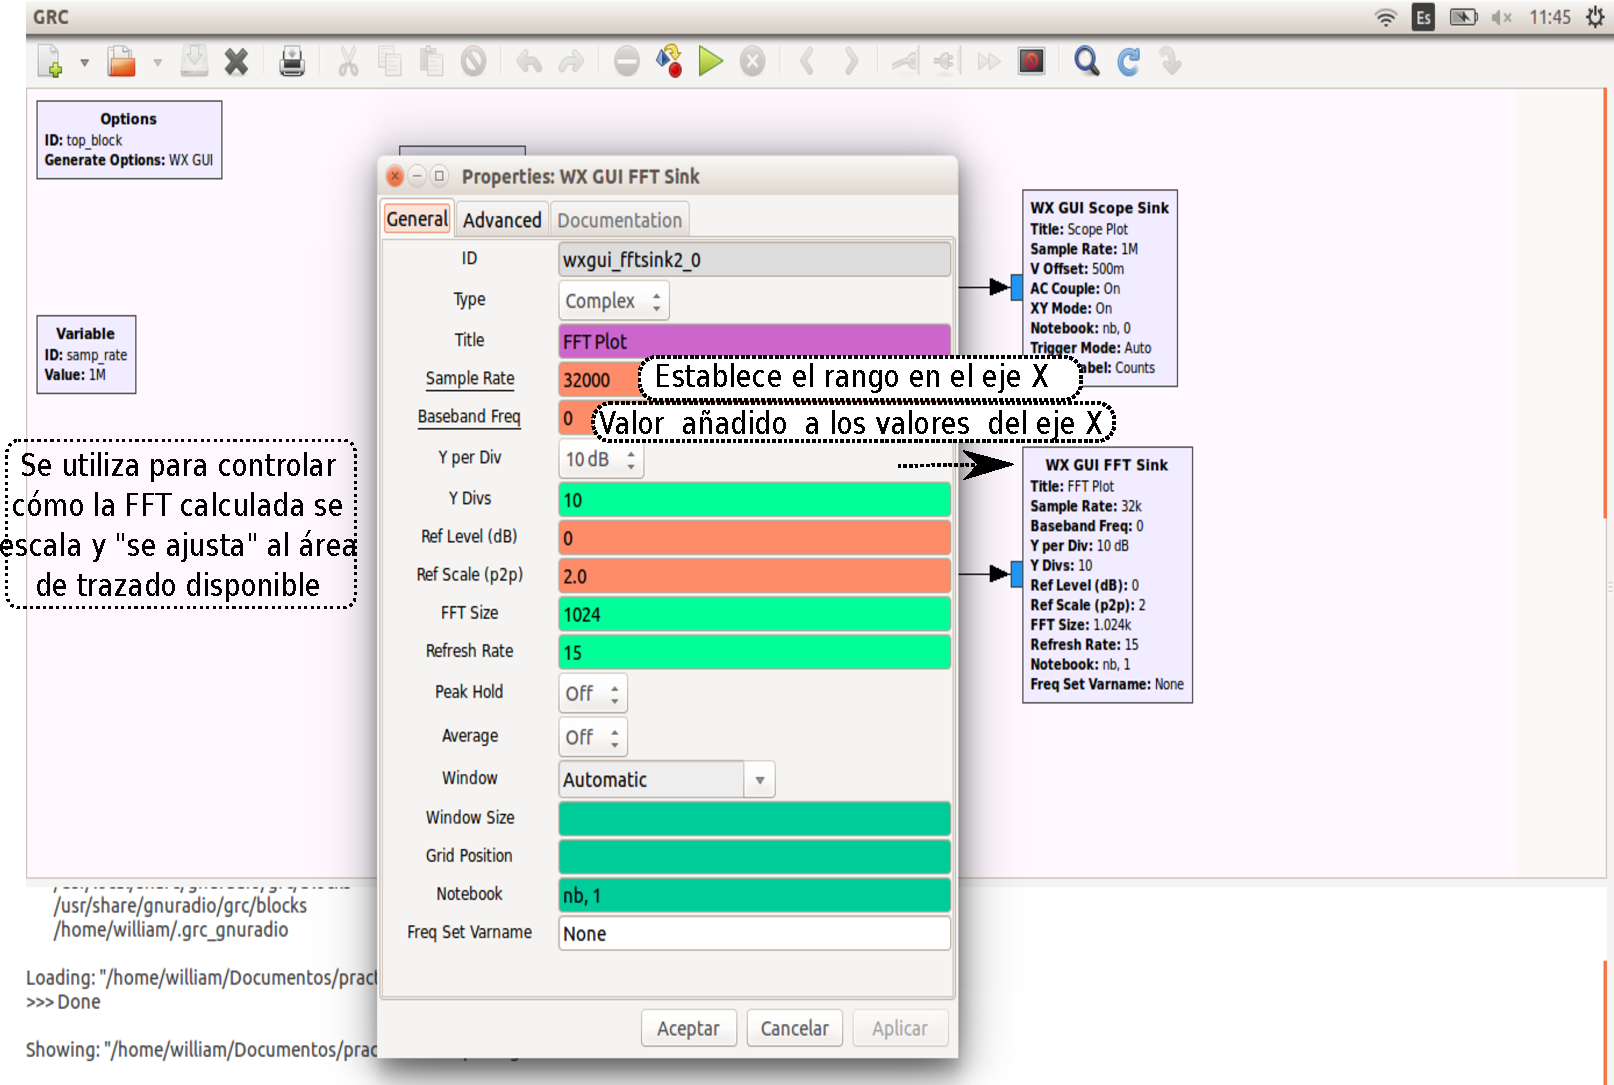
\includegraphics[width=0.85\textwidth]{parte1/lab2/pdf/lab2_7.pdf}
\end{figure}
\end{frame}
%--------------------------------

\begin{frame}{Osciloscopio y FFT\index{WX GUI FFT Sink}}
\begin{figure}[H]
\centering
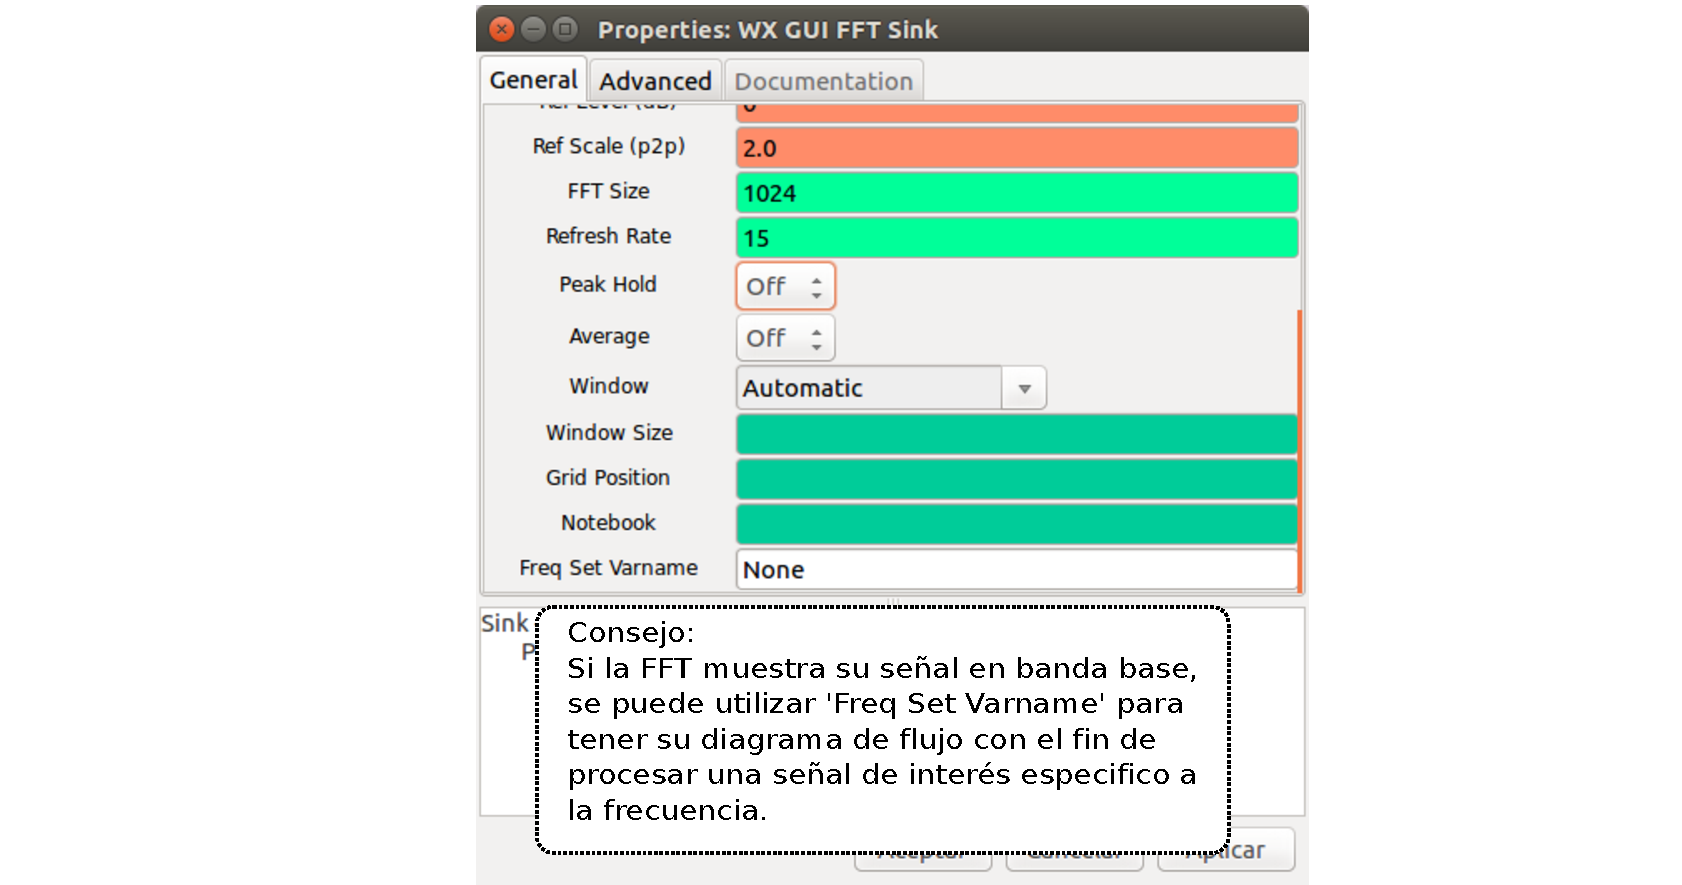
\includegraphics[width=1.1\textwidth]{parte1/lab2/pdf/lab2_8.pdf}
\end{figure}
\end{frame}
%--------------------------------

\begin{frame}{Osciloscopio y FFT\index{WX GUI FFT Sink}}
\begin{figure}[H]
\vspace{-3mm}
\centering
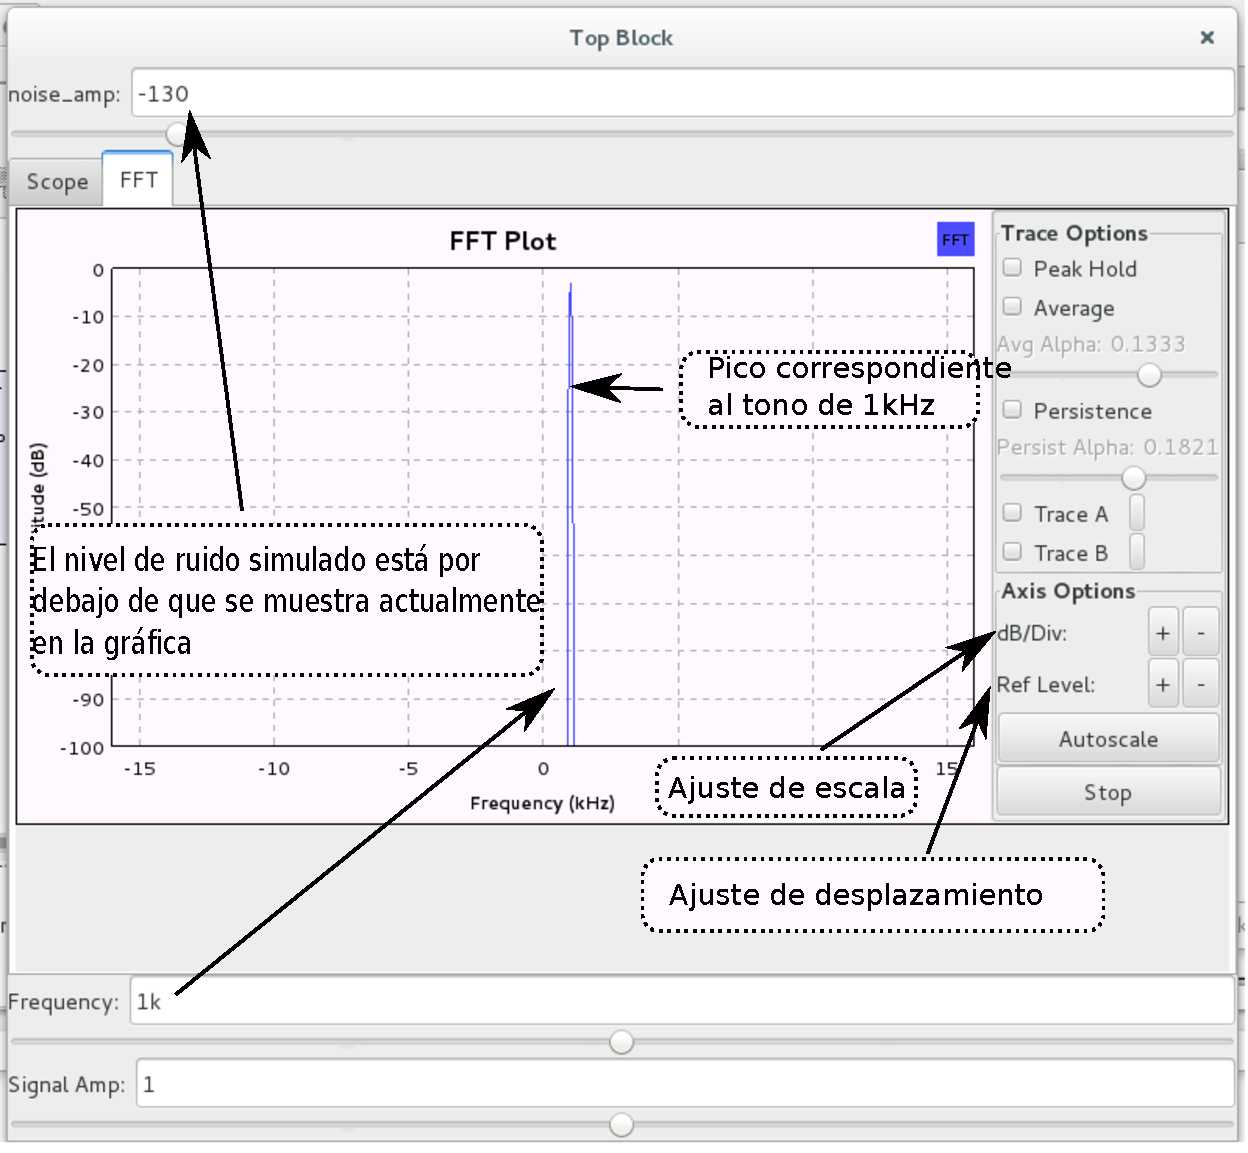
\includegraphics[width=0.7\textwidth]{parte1/lab2/pdf/lab2_9.pdf}
\end{figure}
\end{frame}
%--------------------------------

\begin{frame}{Osciloscopio y FFT}
\begin{figure}[H]
\vspace{-3mm}
\centering
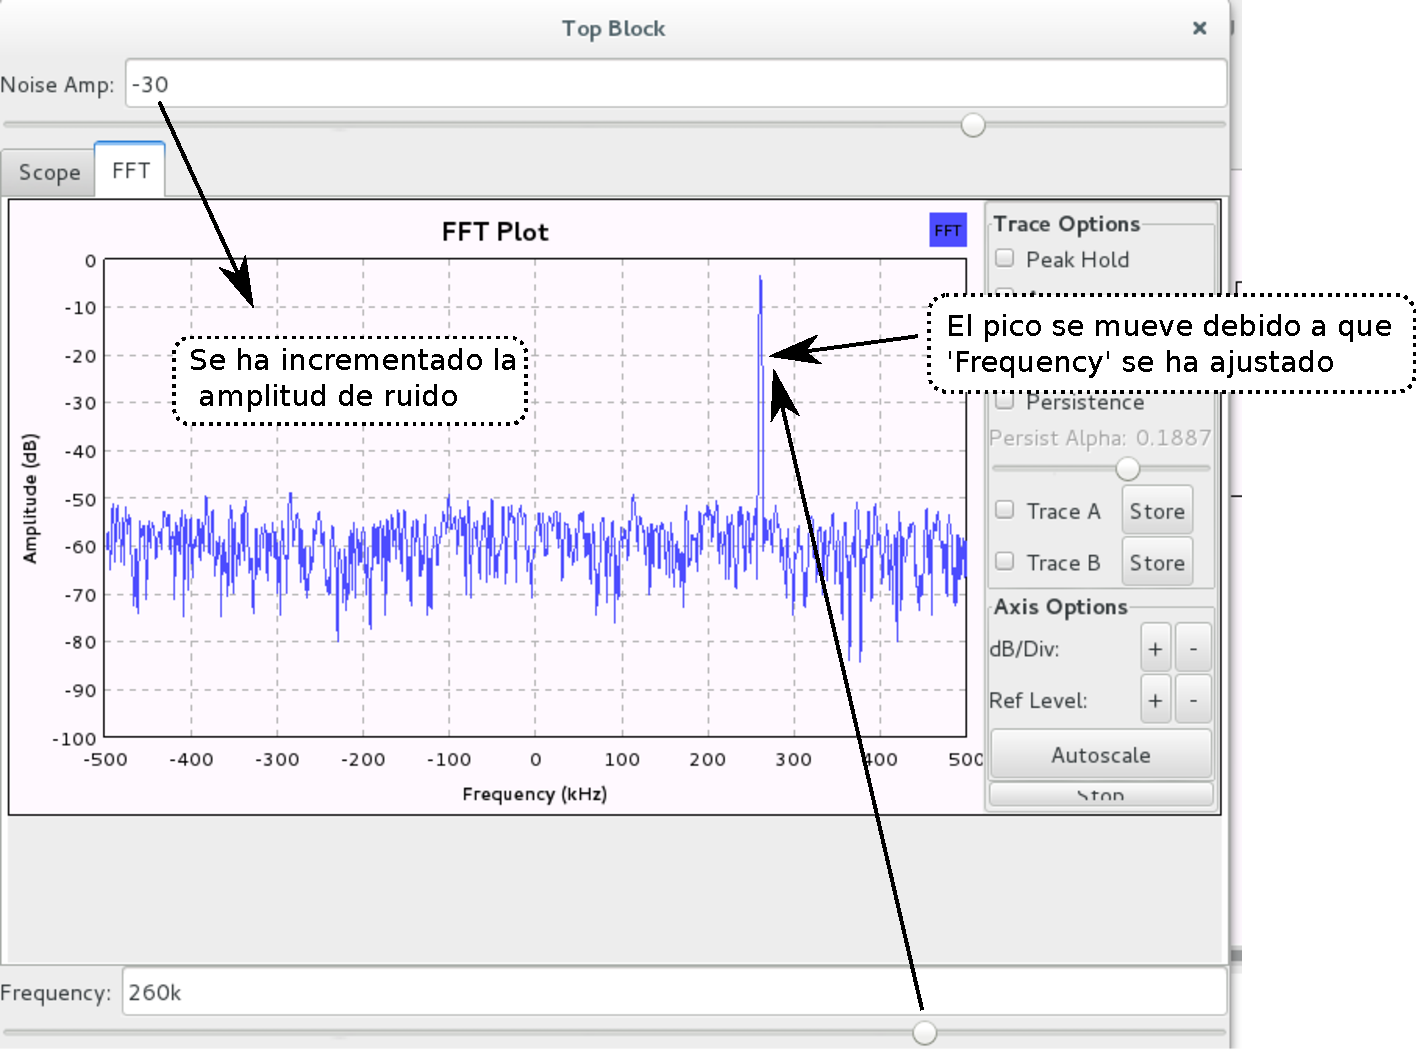
\includegraphics[width=0.85\textwidth]{parte1/lab2/pdf/lab2_10.pdf}
\end{figure}
\end{frame}
%--------------------------------

\begin{frame}{Osciloscopio y FFT}
\begin{figure}[H]
\vspace{-3mm}
\centering
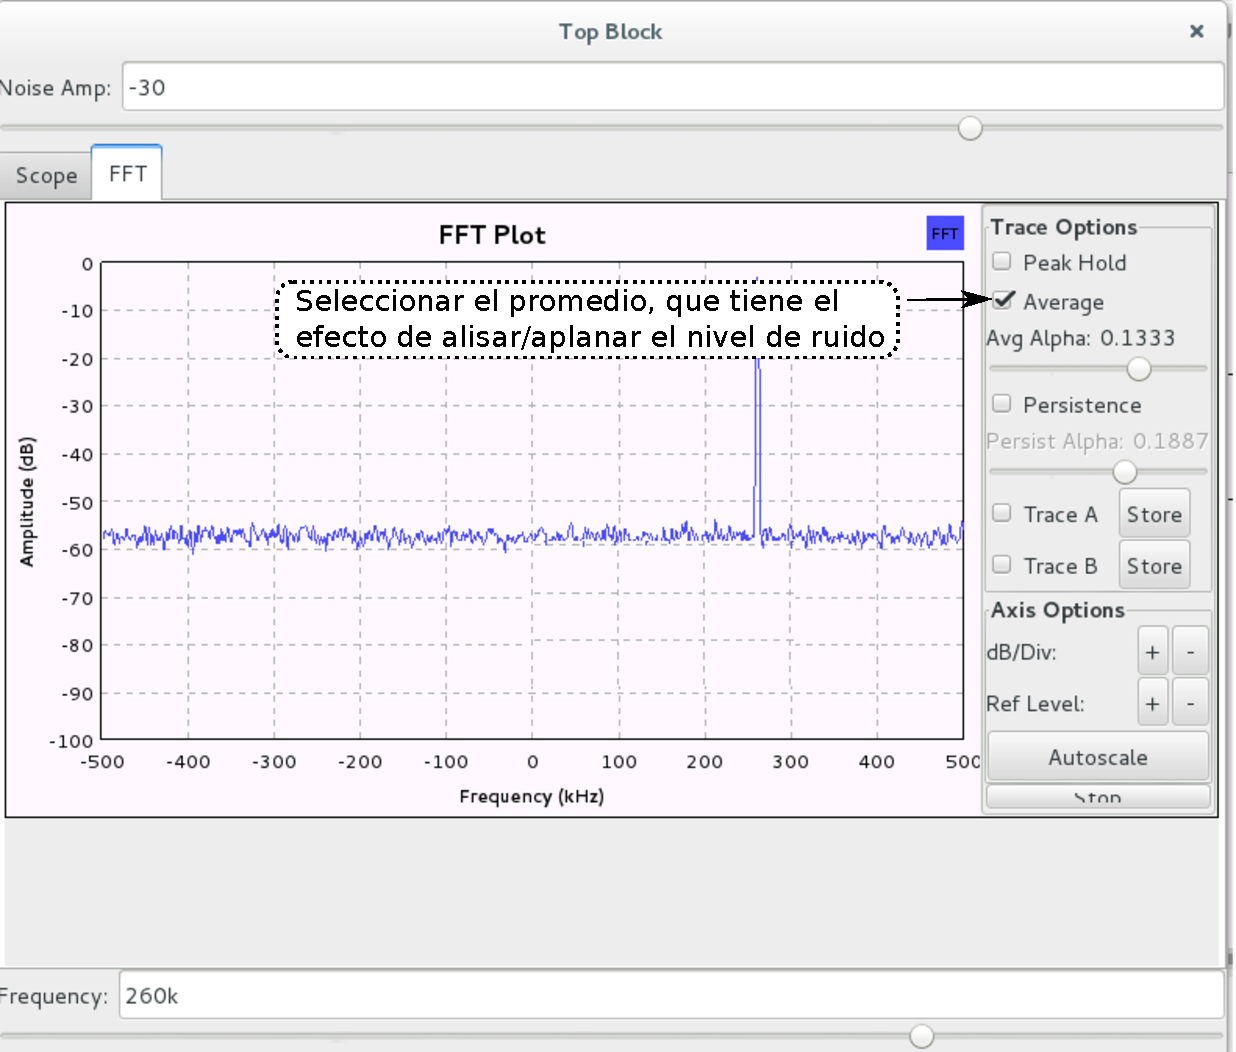
\includegraphics[width=0.75\textwidth]{parte1/lab2/pdf/lab2_11.pdf}
\end{figure}
\end{frame}
%--------------------------------

\begin{frame}{Osciloscopio y FFT}
\begin{figure}[H]
\vspace{-3mm}
\centering
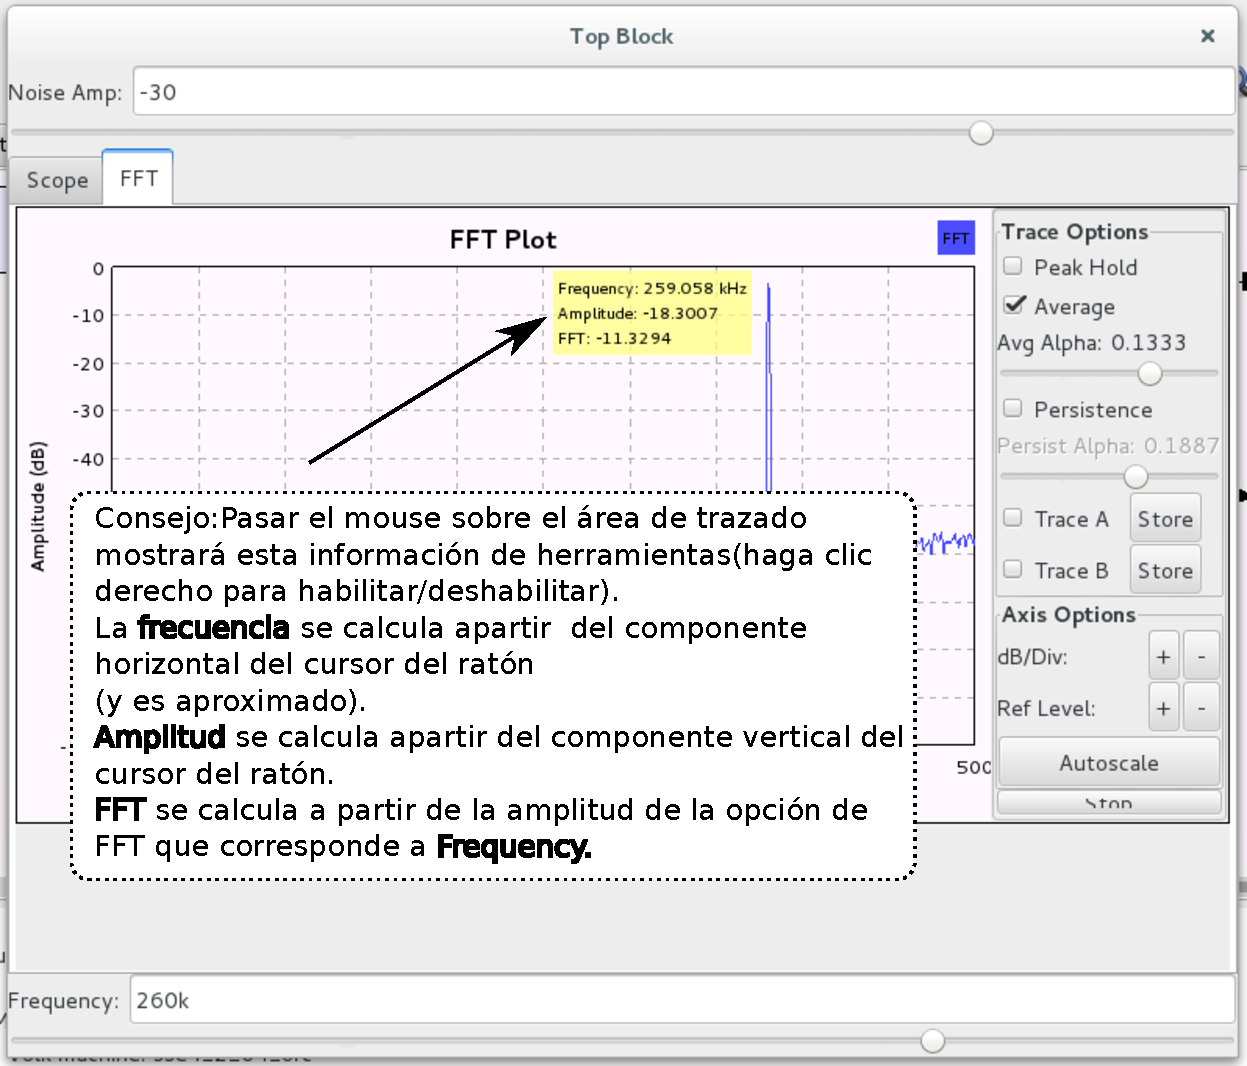
\includegraphics[width=0.75\textwidth]{parte1/lab2/pdf/lab2_12.pdf}
\end{figure}
\end{frame}
%--------------------------------

\begin{frame}{Osciloscopio y FFT}
\begin{figure}[H]
\centering
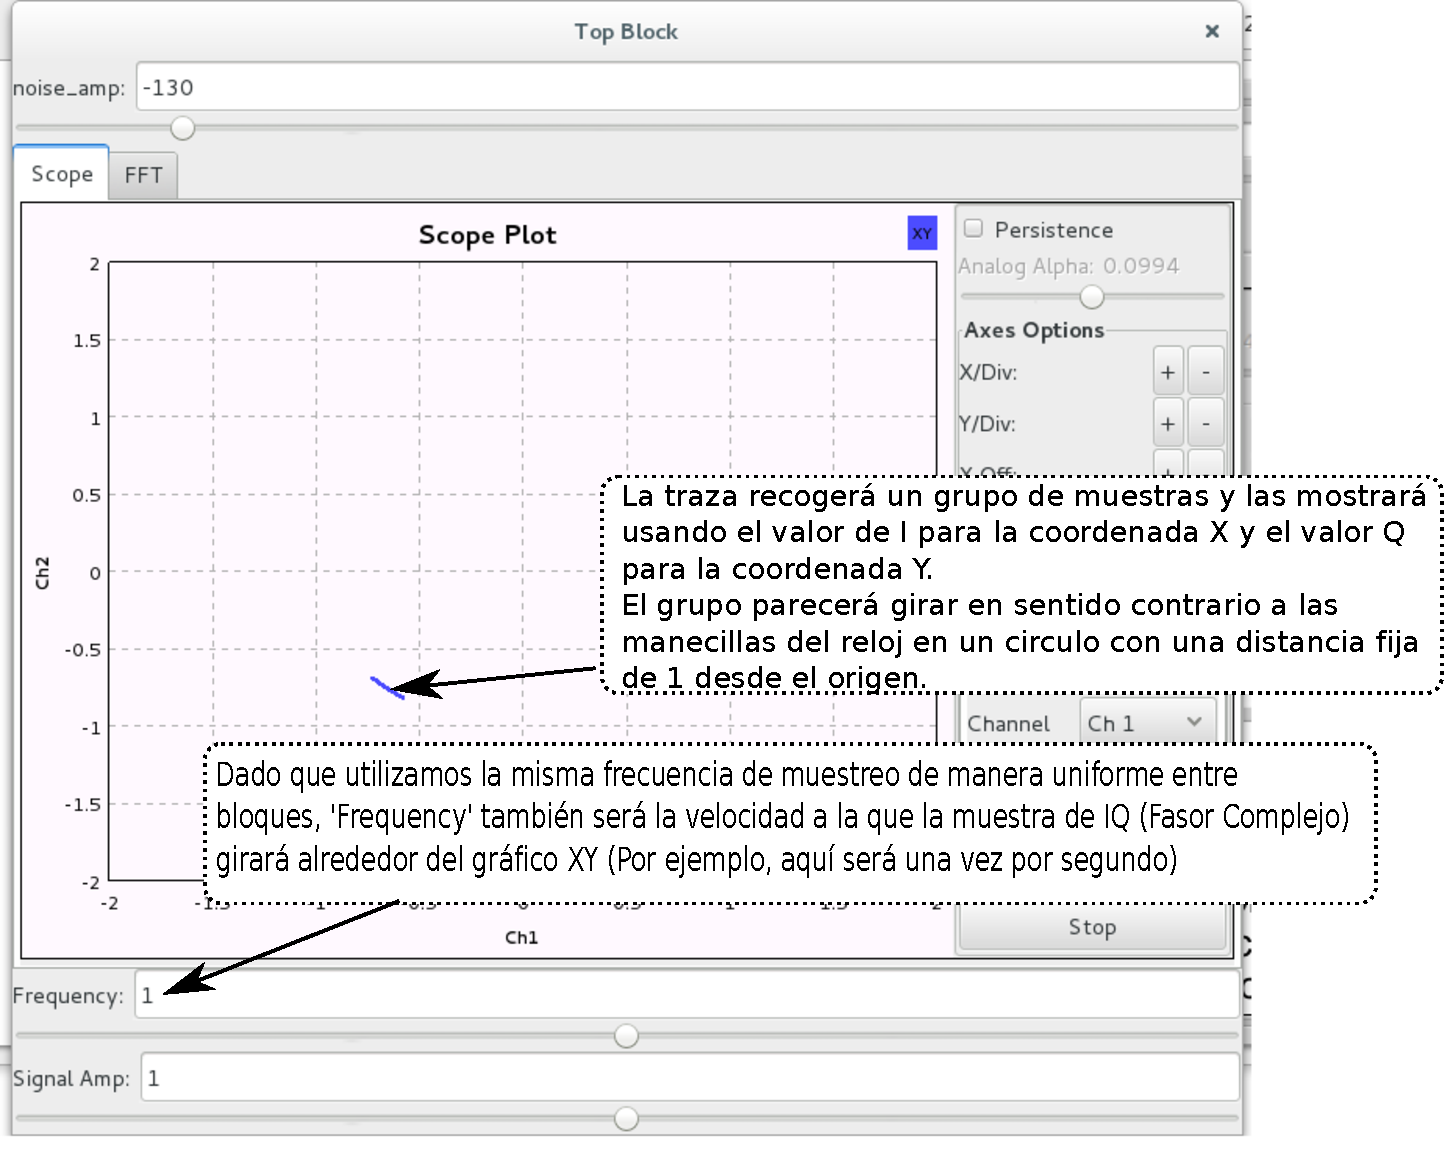
\includegraphics[width=0.75\textwidth]{parte1/lab2/pdf/lab2_13.pdf}
\end{figure}
\end{frame}
%--------------------------------

\begin{frame}{Osciloscopio y FFT}
\begin{figure}[H]
\vspace{-3mm}
\centering
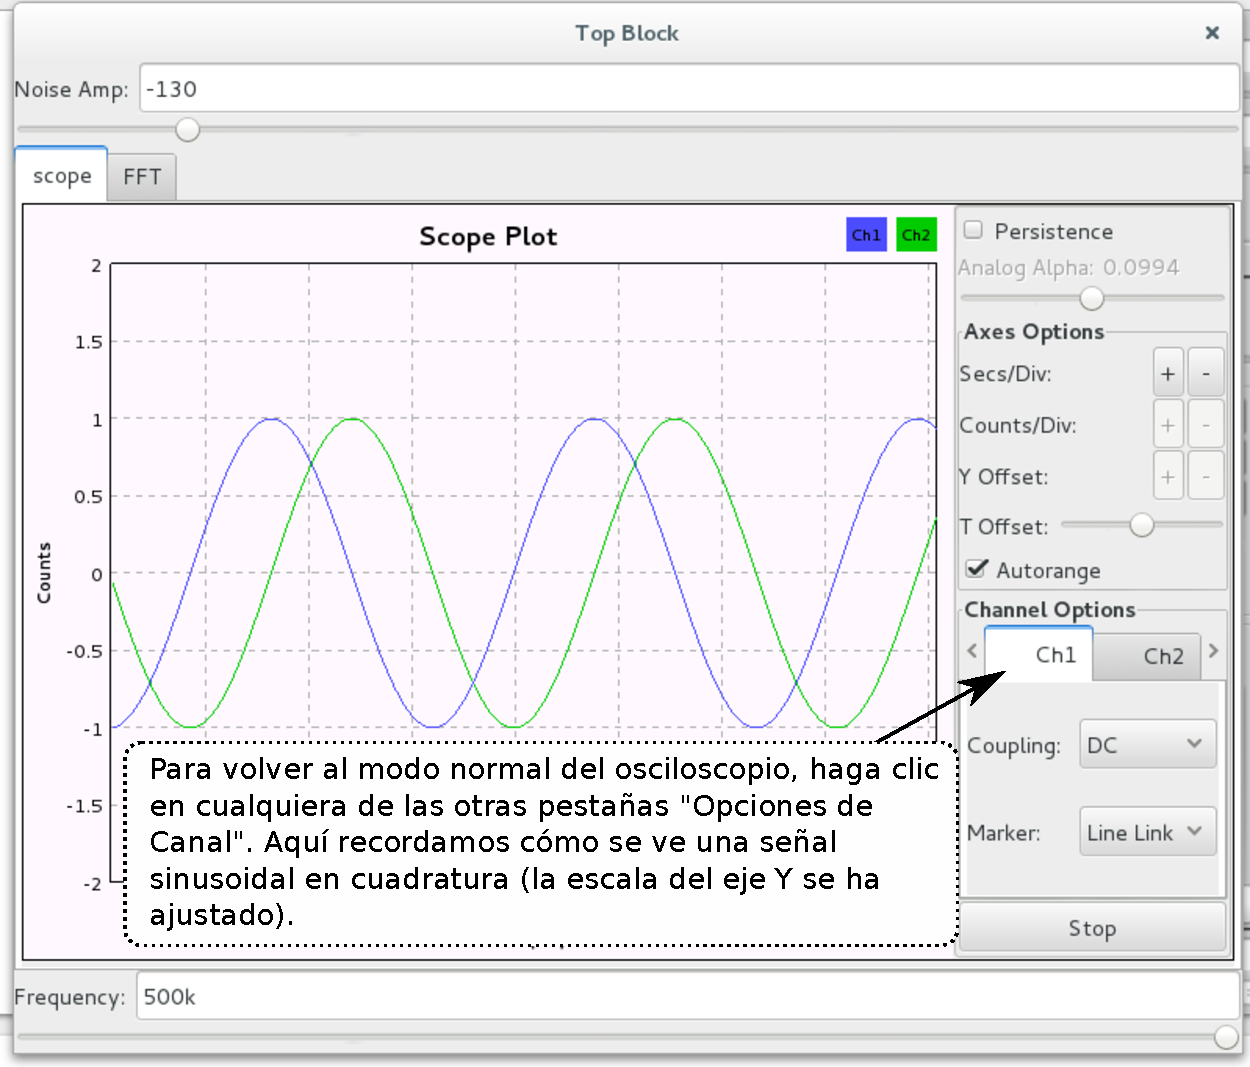
\includegraphics[width=0.75\textwidth]{parte1/lab2/pdf/lab2_14.pdf}
\end{figure}
\end{frame}
%--------------------------------

\begin{frame}{Osciloscopio y FFT}
\begin{figure}[H]
\vspace{-3mm}
\centering
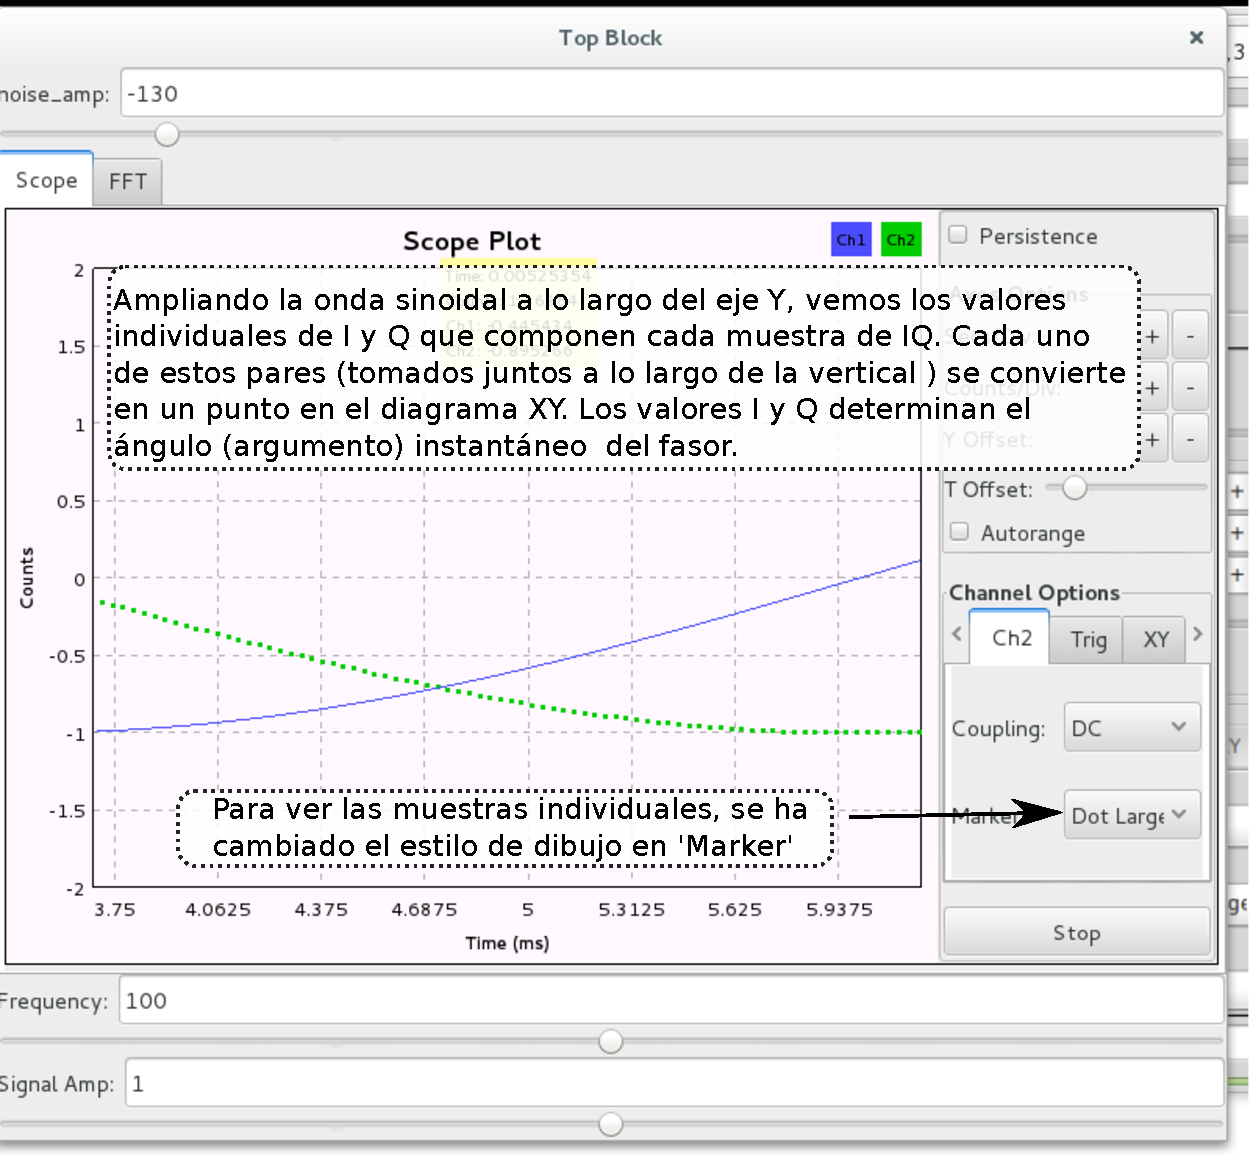
\includegraphics[width=0.7\textwidth]{parte1/lab2/pdf/lab2_15.pdf}
\end{figure}
\end{frame}
%--------------------------------

\begin{frame}{Osciloscopio y FFT}
\begin{figure}[H]
\centering
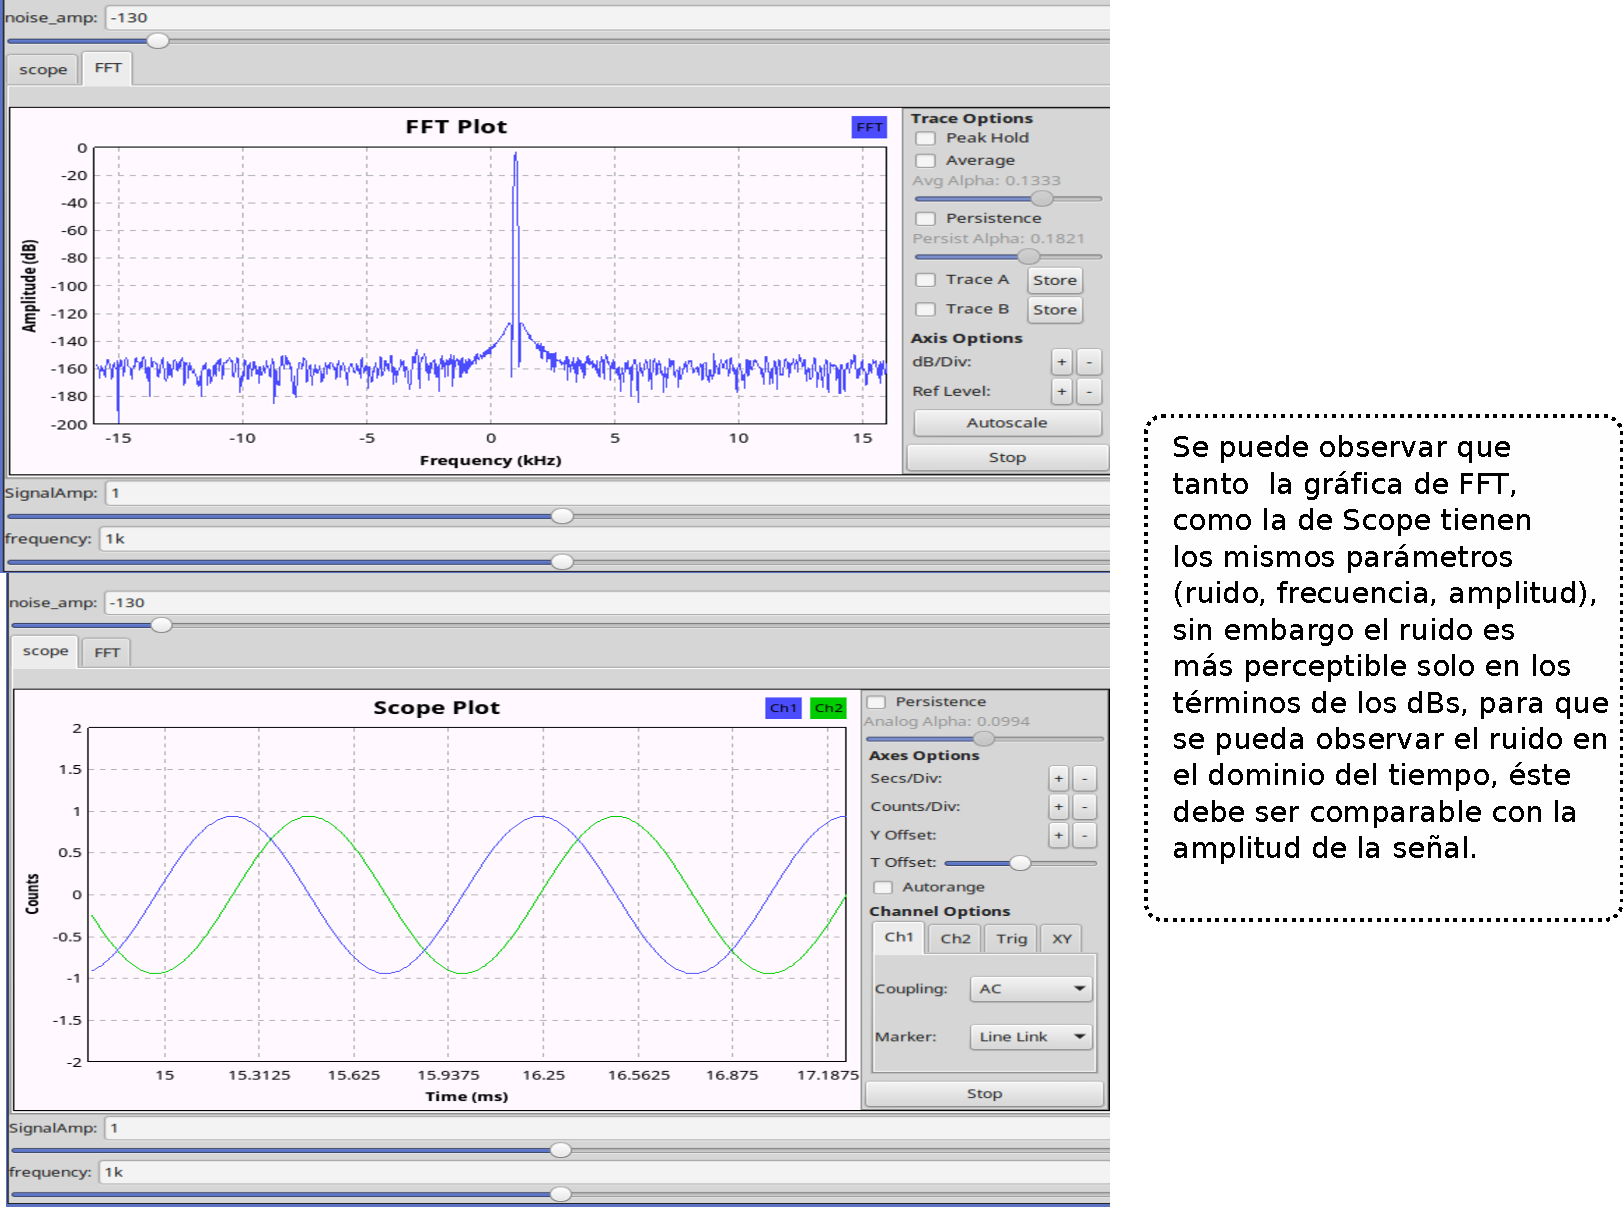
\includegraphics[width=\textwidth, height=0.58\textwidth]{parte1/lab2/pdf/lab2_16.pdf}
\end{figure}
\end{frame}
%--------------------------------

%///////////////////////////////////////////////////////////////

\subsection{Lab3: Audio}
%*********************
\begin{frame}{}

\pgfdeclareimage[width=\paperwidth,height=\paperheight]{bg}{imagenes/fondo_lab}
\setbeamertemplate{background}{\pgfuseimage{bg}}

\bfseries{\textrm{\LARGE Lab3\\ \Large Audio}}
\raggedright
\end{frame}
%*********************

\begin{frame}{Audio \index{Audio}}

\pgfdeclareimage[width=\paperwidth,height=\paperheight]{bg}{imagenes/fondo3}
\setbeamertemplate{background}{\pgfuseimage{bg}}


En esta práctica se generará un tono desde la tarjeta de sonido de la
computadora, originado desde el software y emitido a través de los parlantes
del computador, dicha señal será visualizada desde un osciloscopio, un FFT, y
diagrama de cascada (espectrograma), realizando pruebas de ``loopback'' usando el
micrófono de la computadora.

\end{frame}
%----------------

\begin{frame}{Diagrama:  ``emisión de audio desde la computadora''\index{Audio}}

\begin{figure}

\begin{center}
\vspace{-0.3cm}
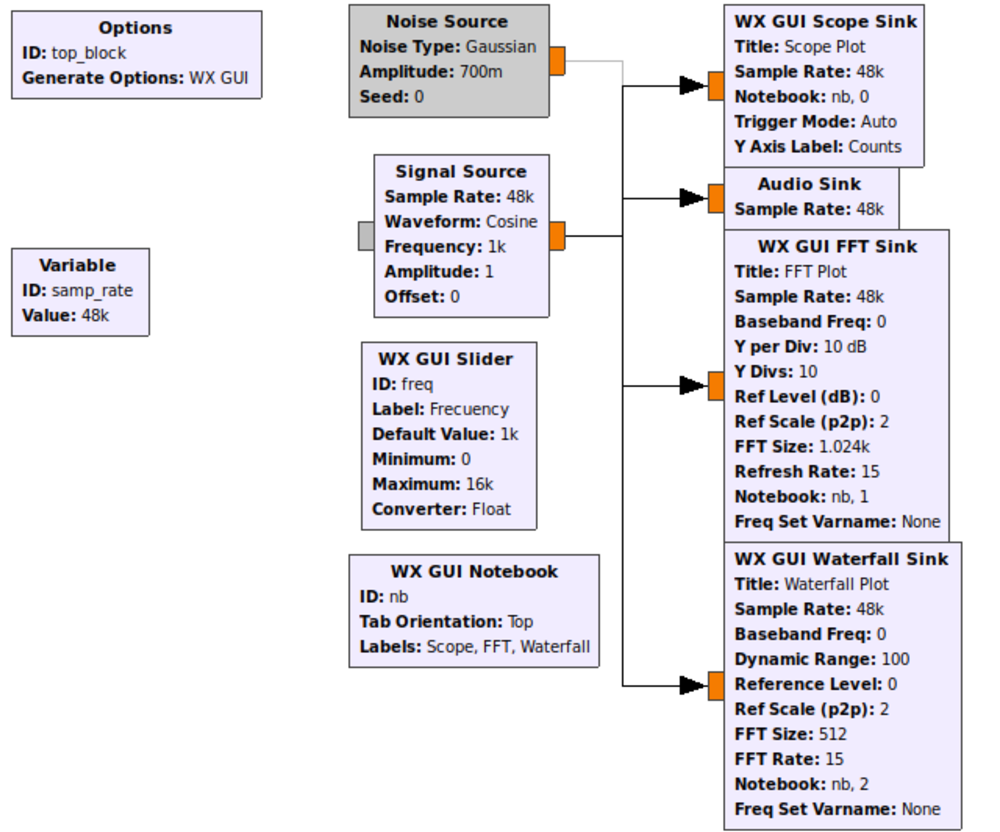
\includegraphics[width=.7\textwidth]{parte1/lab3/pdf/lab3_1.pdf}
\end{center}
\end{figure}

\end{frame}
%----------------

\begin{frame}{Diagrama:  ``emisión de audio desde la computadora''\index{Audio}}

\begin{figure}

\begin{center}
\vspace{-2mm}
    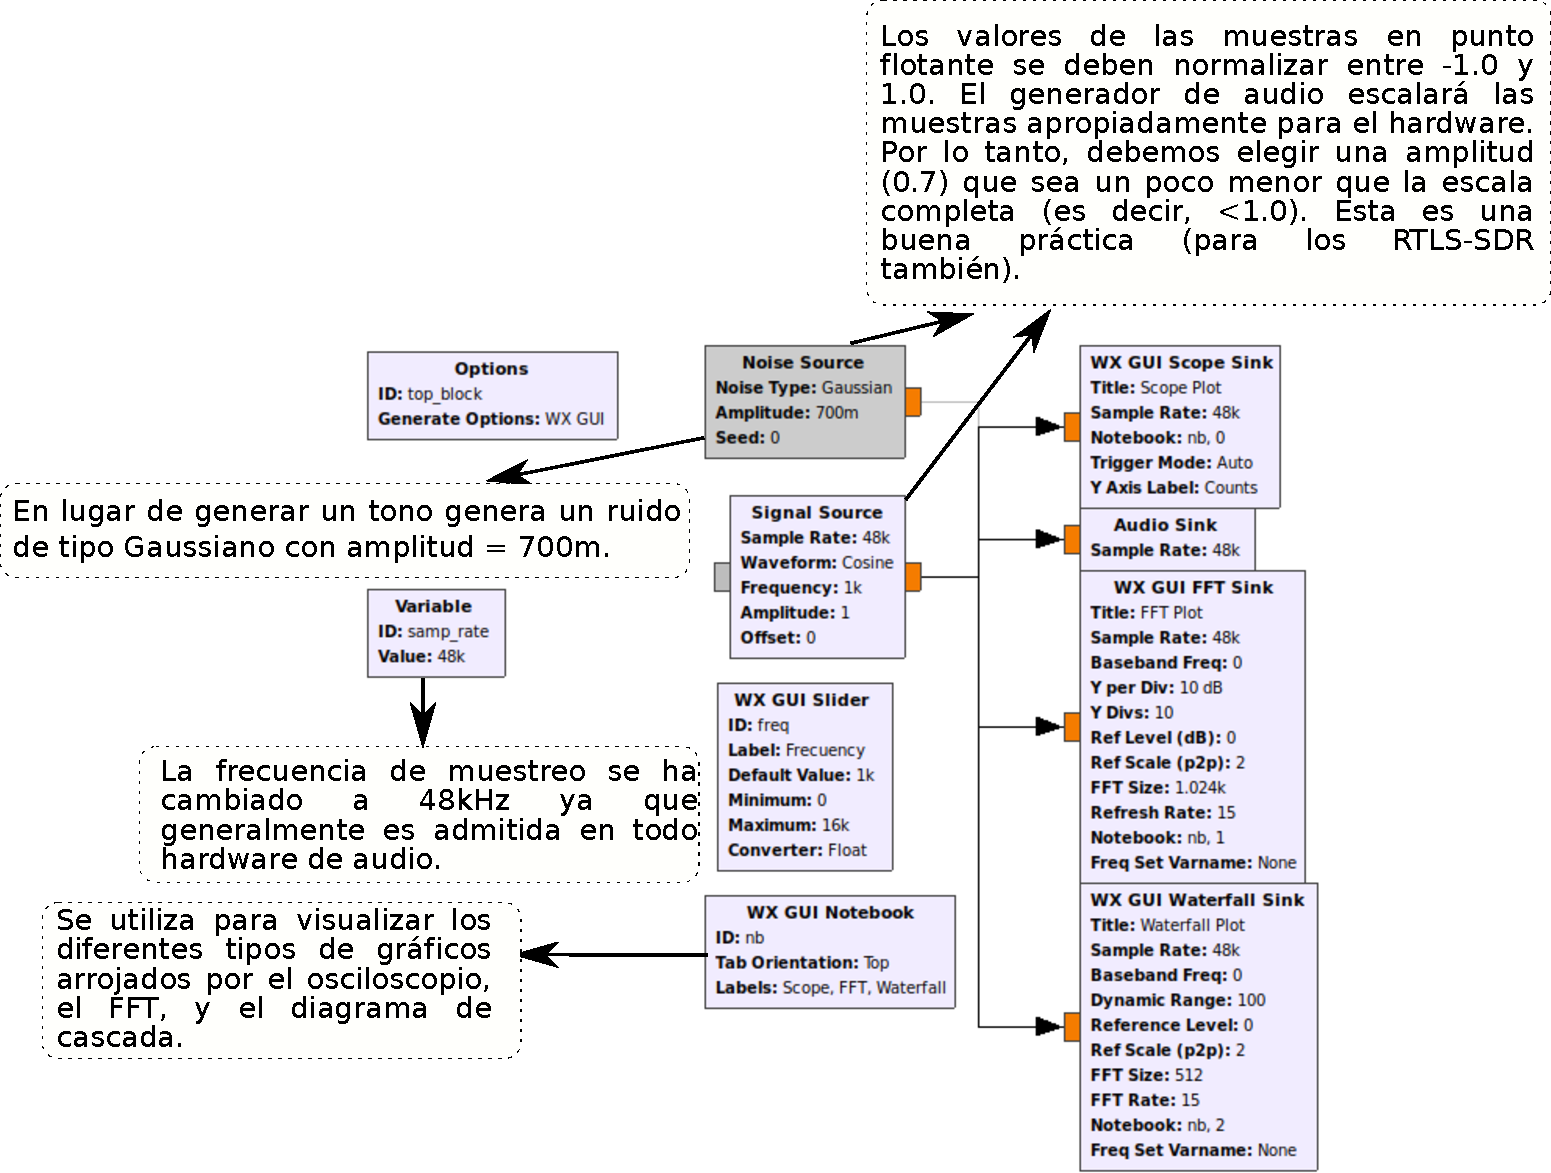
\includegraphics[width=.85\textwidth]{parte1/lab3/pdf/lab3_2.pdf}
\end{center}
\end{figure}

\end{frame}
%----------------

\begin{frame}{Diagrama:  ``emisión de audio desde la computadora''\index{Audio}}

\begin{figure}

\begin{center}
\vspace{-1mm}
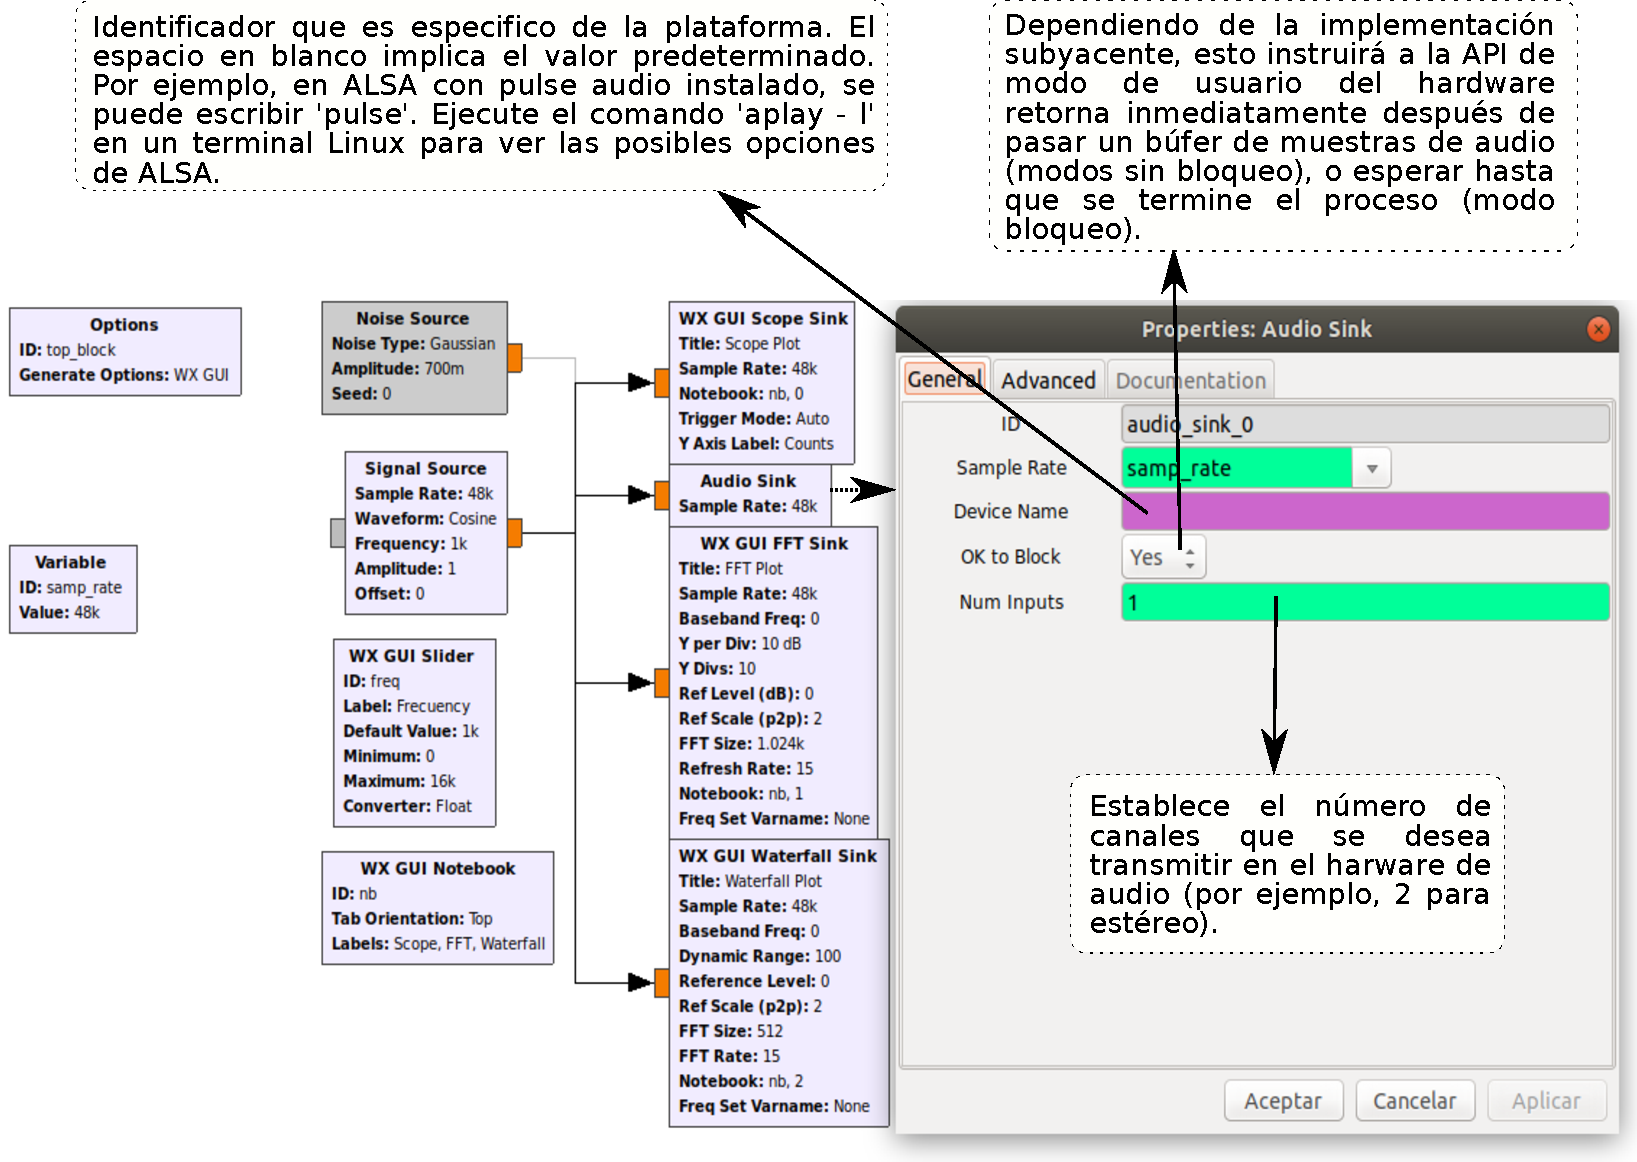
\includegraphics[width=.92\textwidth]{parte1/lab3/pdf/lab3_3.pdf}
\end{center}
\end{figure}

\end{frame}
%----------------

\begin{frame}{Diagrama:  ``emisión de audio desde la computadora''\index{Audio}}

\begin{figure}

\begin{center}
\vspace{-8mm}
\includegraphics[width=1.05\textwidth]{parte1/lab3/pdf/lab3_4.pdf}
\end{center}
\end{figure}

\end{frame}
%----------------

\begin{frame}{Audio\index{Audio}}

Es importante saber que:\\
\begin{itemize}
    \item
    {Cuando Audio Sink es el único dispositivo hardware en el diagrama de bloques capaz de generar audio, el modo de bloqueo (‘OK to Block’) aplicará un regulador a la producción de muestras del sample\_rate, para que opere eficazmente al reproducir el sonido\cite{Seeber2014}.}
    \item
    {Esto puede ser problemático si la fuente del diagrama de flujo es, por ejemplo, un RTL-SDR. La fuente es también un hardware que tiene su propio reloj interno y será regulado a la tasa de producción de las muestras, mientras que el Audio Sink regula el uso con su propio reloj no sincronizado. Esto se llama el problema de “dos relojes".}
\end{itemize}
\end{frame}
%----------------

\begin{frame}{Audio\index{Audio}}
\begin{itemize}
    \item 
    {Para solucionar este problema de dos relojes, se coloca un regulador de audio en modo sin bloqueo (no dar click ‘Botón de Bloqueo’) de tal forma que nunca interrumpa el diagrama de bloque (es decir, no aplicar el regulador controlado). Esto usará muestras de forma normal, pero si hay un exceso (por ejemplo, el RTL-SDR está produciendo muestras un poco más rápido de lo que el Audio Sink puede usar), se perderán las muestras (podría causar fallas de audio).}
    \item 
    {Esto no soluciona el caso en el que las muestras se producen más lentamente que la tasa de uso del Audio Sink (esto producirá una ejecución lenta: el audio sonará agitado y se imprimirá ‘aU’ en la ventana de registro).}
\end{itemize}



\end{frame}
%----------------

\begin{frame}{Audio\index{Audio}}

\begin{figure}

\begin{center}
\vspace{-7mm}
\includegraphics[width=\textwidth, height=0.6\paperheight]{parte1/lab3/pdf/lab3_5.pdf}
\end{center}
\end{figure}
%\tiny
\vspace{-4mm}
La misma onda seno de las prácticas anteriores, pero ahora se puede escuchar emitida por los parlantes del computador.
\end{frame}
%----------------

\begin{frame}{Audio\index{Audio}}

\begin{figure}

\begin{center}
\vspace{-6mm}
\includegraphics[width=0.8\textwidth]{parte1/lab3/pdf/lab3_6.pdf}
\end{center}
\end{figure}
\vspace{-3mm}

Visualiza el FFT que se desplaza en el tiempo mediante el diagrama de cascada (espectrograma) de la señal emitida. Se añade un bloque de prueba por medio de un generador de señales y un variador deslizante con lo cual se escucha el tono variado en el Audio Sink y poder ver la variación de la frecuencia en el diagrama de cascada.
\end{frame}
%----------------

\begin{frame}{Diagrama: recepción de audio\index{Audio}}

\begin{figure}

\begin{center}
%\vspace{-5mm}
\includegraphics[width=.73\textwidth]{parte1/lab3/pdf/lab3_7.pdf}
\end{center}
\end{figure}

\end{frame}
%----------------

\begin{frame}{Audio\index{Audio}}

\begin{figure}
\begin{center}
\vspace{-8mm}
\includegraphics[width=\textwidth]{parte1/lab3/pdf/lab3_8.pdf}
\end{center}
\end{figure}

Muestra las diferentes señales presentes en el entorno captadas por la tarjeta de audio de la computadora a través del micrófono.

\end{frame}
%----------------

\begin{frame}{Diagrama: prueba con aproximación de “loopback”\index{Audio}}

\begin{figure}
\begin{center}
\vspace{-6mm}
\includegraphics[width=\textwidth, height=0.6\paperheight]{parte1/lab3/pdf/lab3_9.pdf}
\end{center}
\end{figure}
\vspace{-5mm}
Ejecutando el programa generador de onda sinusoidal al mismo tiempo, y cambiando la frecuencia. Se trata de una prueba aproximada de “loopback" en la que el micrófono de la computadora escucha sus altavoces.

\end{frame}
%----------------

\begin{frame}{Audio\index{Audio}}

\begin{figure}
\begin{center}
\vspace{-8mm}
\includegraphics[width=\textwidth, height=0.6\paperheight]{parte1/lab3/pdf/lab3_10.pdf}
\end{center}
\end{figure}
\vspace{-5mm}
Con la realimentación de las entradas micrófono-altavoces y generación de señal a través de la tarjeta de audio de la computadora.

\end{frame}
%---------------
  

%///////////////////////////////////////////////////////////////

\subsection{Lab4: Modulación ASK en GRC}

%*********************
\begin{frame}{}

\pgfdeclareimage[width=\paperwidth,height=\paperheight]{bg}{imagenes/fondo_lab}
\setbeamertemplate{background}{\pgfuseimage{bg}}

\bfseries{\textrm{\LARGE Lab4\\ \Large Modulación ASK en GRC}}
\raggedright
\end{frame}
%*********************

%--------------------------

\begin{frame}{Modulación ASK en GRC}


\pgfdeclareimage[width=\paperwidth,height=\paperheight]{bg}{imagenes/fondo3}
\setbeamertemplate{background}{\pgfuseimage{bg}}

  \begin{itemize}
  \item {
En esta práctica se hace uso de la  Modulación por desplazamiento de amplitud (ASK) este es un esquema de modulación digital en el que la amplitud de la onda portadora se cambia con respecto a la señal de información, manteniendo la fase y la frecuencia de constantes. Para el presente laboratorio, se utilizó BASK, el cual tiene el mismo comportamiento, pero utilizando bits. Donde su comportamiento es descrito por la siguiente ecuación:

\begin{equation*}
S(t) = Am(t)cos(wt)
\end{equation*}

  }
  \item {
El diagrama de bloques en GRC consiste en la multiplicación de una señal de información con una portadora, que corresponde a una señal coseno de diez veces la frecuencia de la información. La frecuencia de muestreo debe ser mayor que el doble de la frecuencia máxima de la señal de datos.
  }
  \end{itemize}
\end{frame}
%---------------------------

\begin{frame}{Modulación ASK en GRC}

\begin{figure}[H]
\centering
\includegraphics[width=\textwidth]{parte1/lab4/pdf/lab4_1.pdf}
\end{figure}
Diagrama de bloques en GNU radio, para generar una modulación ASK entre dos señales.
\end{frame}
%--------------------

\begin{frame}{Modulación ASK en GRC}
\vspace{-1cm}
\begin{figure}[H]
\centering
\includegraphics[width=1.1\textwidth]{parte1/lab4/pdf/lab4_2.pdf}
\end{figure}
\end{frame}
%_---------------------

\begin{frame}{Modulación ASK en GRC}
\vspace{-1.5cm}
\begin{figure}[H]
\centering
\includegraphics[width=1.1\textwidth]{parte1/lab4/pdf/lab4_3.pdf}
\end{figure}
\end{frame}
%_---------------------

\begin{frame}{Modulación ASK en GRC}

  \begin{itemize}
  \item {
La Modulación por desplazamiento de frecuencia (FSK) es una técnica de modulación digital, utilizada para la transmisión de datos. Para BFSK que corresponde al mismo proceso, pero con datos binarios, se utilizan dos frecuencias diferentes para transmitir dos señales, es decir 0 y 1. como se puede ver a continuación:

\begin{equation*}
S_{1}(t) = Acos(w_{1}t)
\end{equation*}

\begin{equation*}
S_{2}(t) = Acos(w_{2}t)
\end{equation*}

  }
  \item {
El diagrama de boques en GRC se utilizaron dos señales coseno como portadora de amplitud 1, y frecuencias de 1Khz y 10Khz. La señal 1 es representada por una onda cuadrada, y la señal 0 es obtenida restándole 1 a la señal cuadrada. Posteriormente se multiplican las señales 0 y 1 con las portadoras y luego se suman obteniendo la modulación FSK.
  }
  \end{itemize}
\end{frame}
%---------------------------


\begin{frame}{Modulación ASK en GRC}
\vspace{-8mm}
\begin{figure}[H]
\centering
\includegraphics[width=\textwidth]{parte1/lab4/pdf/lab4_4.pdf}
\end{figure}
\end{frame}
%_---------------------

\begin{frame}{Modulación ASK en GRC}
\begin{figure}[H]
\centering
\includegraphics[width=\textwidth]{parte1/lab4/pdf/lab4_5.pdf}
\end{figure}
\end{frame}
%_---------------------

\begin{frame}{Modulación ASK en GRC}
\begin{figure}[H]
\centering
\includegraphics[width=\textwidth]{parte1/lab4/pdf/lab4_6.pdf}
\end{figure}
\end{frame}
%_---------------------

\begin{frame}{Modulacion ASK en GRC}

  \begin{itemize}
  \item {
La Modulación por desplazamiento de fase (PSK) es un esquema de modulación digital donde se varía la fase de la señal, manteniendo la frecuencia y la amplitud constante. Para la modulación PSK se usan dos señales con fases diferentes y frecuencias iguales, estas se multiplican con la señal 0 o 1 de los datos como se muestra a continuación:

\begin{equation*}
S_{1}(t) = Acos(wt)
\end{equation*}

\begin{equation*}
S_{2}(t) = Acos(wt)
\end{equation*}

  }
  \item {
El diagrama de boques en GRC se utiliza una señal coseno de 50000 Hz y la amplitud pico de 1, y otra onda sinusoidal de igual frecuencias y amplitud. Similar a BFSK se representa la señal 1 con la onda cuadrada de frecuencia 5000 Hz y el 0 por la resta de la constante.
  }
  \end{itemize}
\end{frame}
%---------------------------

\begin{frame}{Modulación ASK en GRC}
\begin{figure}[H]
\centering
\includegraphics[width=\textwidth]{parte1/lab4/pdf/lab4_7.pdf}
\end{figure}
\end{frame}
%_---------------------

\begin{frame}{Modulación ASK en GRC}
\begin{figure}[H]
\centering
\includegraphics[width=\textwidth]{parte1/lab4/pdf/lab4_8.pdf}
\end{figure}
\end{frame}
%_---------------------
\begin{frame}{Modulación ASK en GRC}
\begin{figure}[H]
\centering
\includegraphics[width=\textwidth]{parte1/lab4/pdf/lab4_9.pdf}
\end{figure}
\end{frame}
%_---------------------   

%///////////////////////////////////////////////////////////////

\subsection{Lab5: Modulación BPSK en GRC}

%*********************
\begin{frame}{}

\pgfdeclareimage[width=\paperwidth,height=\paperheight]{bg}{imagenes/fondo_lab}
\setbeamertemplate{background}{\pgfuseimage{bg}}

\bfseries{\textrm{\LARGE Lab5\\ \Large Modulación BPSK en GRC}}
\raggedright
\end{frame}
%*********************

%--------------------------

\begin{frame}{Modulación BPSK en GRC}


\pgfdeclareimage[width=\paperwidth,height=\paperheight]{bg}{imagenes/fondo3}
\setbeamertemplate{background}{\pgfuseimage{bg}}


En esta práctica se hace uso de la modulación de desplazamiento de fase de 2 símbolos. Es el más sencillo de todos, puesto que solo emplea 2 símbolos, con 1 bit de información cada uno. Es también la que presenta mayor inmunidad al ruido, puesto que la diferencia entre símbolos es máxima (180º). Dichos símbolos suelen tener un valor de salto de fase de 0º para el 1 y 180º para el 0, como se muestra en un diagrama de constelación.
  

\end{frame}
%---------------------------

\begin{frame}{Modulación BPSK en GRC}

\begin{figure}
  \centering
   \includegraphics[width=\textwidth]{parte1/lab5/pdf/lab5_1.pdf}
  \end{figure}
  
\end{frame}
%------------------------

\begin{frame}{Modulación BPSK en función del tiempo}
\begin{figure}[H]
\centering
\includegraphics[width=.7\textwidth]{parte1/lab5/pdf/lab5_2.pdf}
\end{figure}
Convierte el flujo de datos digital en señal analógica de banda base (muestreada) utilizando el filtro FIR de interpolación.
\end{frame}
%------------------------

\begin{frame}{Modulación BPSK en GRC}
\begin{figure}[H]
\centering
\includegraphics[width=.7\textwidth]{parte1/lab5/pdf/lab5_3.pdf}
\end{figure}
\end{frame}
%------------------------

\begin{frame}{Modulación BPSK en función del tiempo}
\begin{figure}[H]
\centering
\includegraphics[width=.8\textwidth]{parte1/lab5/pdf/lab5_4.pdf}
\end{figure}
\end{frame}
%------------------------

\begin{frame}{Modulación BPSK en GRC}
\begin{figure}[H]
\centering
\includegraphics[width=\textwidth]{parte1/lab5/pdf/lab5_5.pdf}
\end{figure}
\end{frame}
%------------------------

\begin{frame}{Modulación BPSK en GRC}
\vspace{-8mm}
\begin{figure}[H]
\centering
\includegraphics[width=.9\textwidth]{parte1/lab5/pdf/lab5_6.pdf}
\end{figure}
\tiny
Se deshabilita el bloque del osciloscopio WX GUI y se habilita el osciloscopio de constelaciones QT GUI , también se debe cambiar en el bloque Options: Generate options: WX GUI por QT GUI para que el bloque de constelaciones funcione.
\end{frame}
%------------------------

\begin{frame}{Constelación BPSK}
\begin{figure}[H]
\centering
\includegraphics[width=\textwidth]{parte1/lab5/pdf/lab5_7.pdf}
\end{figure}
\end{frame}
%------------------------   
%///////////////////////////////////////////////////////////////
